In this chapter, we develop an algorithm for interpretable safety validation that generates failure descriptions in the form of signal temporal logic expressions. A failure description is any statement that defines a set of disturbance trajectories that cause the system to fail and is useful for understanding failure modes, producing failure examples. Failure descriptions are found using expression optimization and evaluated by sampling satisfying trajectories. We introduce a technique for sampling satisfying trajectories of STL specifications by applying a set of linear constraints to the disturbance model which can be done efficiently for independent disturbances and disturbances that are jointly distributed as a Gaussian process. Through experiments in two autonomous driving scenarios, we demonstrate that our interpretable safety validation algorithm can find failure descriptions, and produce a diverse set of failure examples. Failure descriptions may also be used to analyze the sensitivity of the safety of the system with respect to important disturbance parameters. 

\section{Motivation}

% Introduce the problem (motivation)
One of the drawbacks to black-box safety validation techniques approaches is that they do not produce high-level descriptions of failures and instead only produce high-dimensional failure examples. In scenario-based testing, by contrast, each scenario involves semantically similar disturbance trajectories which can provide clues to the source of an error. For example, suppose a black-box safety validation algorithm discovered a failure of an autonomous vehicle driving on the highway. It would not be clear from this one example if the failure was due to perception, planning, control or something else. If, however, we found that the vehicle failed in a scenario designed to test its response to partially occluded stop signs, we would be justified in investigating the perception system. This work tries to bring a greater degree of interpretability to black box safety validation algorithms. 

% The approach we propose
Our approach seeks to find a \emph{failure description} $\varphi$ such that any disturbance trajectory that satisfies the description will cause the system to fail. For falsification, we want to find any such $\varphi$ where
\begin{equation}
    \vec{x} \in \varphi \implies f(\vec{x}) \not \in \psi \text{.}
\end{equation}
For most likely failure analysis we want to find the $\varphi$ that produces failures with high likelihood
\begin{equation}
\max_\varphi \quad \mathbb{E}_{\vec{x} \sim p(\vec{x} \mid \vec{x} \in \varphi)}[p(\vec{x})] \quad\textrm{s.t.}\quad \vec{x} \in E
\end{equation}
where $p(\vec{x} \mid \vec{x} \in \varphi)$ is the probability density of disturbance trajectories that satisfy the description. 

A failure description $\varphi$ contains more information than a single failure example. For example, a single failure description can produce many failure examples by sampling from $p(\vec{x} \mid \vec{x} \in \varphi)$. It also identifies logical features of a disturbance trajectory that are sufficient to cause a failure. As in scenario-based testing, those features may provide clues to the source of the error in the system. Lastly, if the features are low dimensional, they can be used to perform a sensitivity analysis of the safety of the system with respect to the disturbance variables. 


\section{STL Expression Optimization}
This section provides the necessary technical background to understand our approach for STL expression optimization. We first introduce context free grammars as a way to compactly represent signal temporal logic and describe how to sample valid STL expressions. We then describe genetic programming, a technique used to optimize tree-like structures such as STL expressions. Lastly, we introduce the failure description cost function that is used to find optimal failure descriptions.

\subsection{Context-Free Grammars}
\begin{figure}
    \centering
    \begin{forest}{for tree={ minimum size=1cm,}}
        [$\square$ 
            [$t_1$] 
            [$t_2$] 
            [$>$ 
                [$x$]
                [$0$]
            ]
        ]
    \end{forest}
    \caption{Expression tree for $\square_{[t_1, t_2]} x > 0$.}
    \label{fig:stl_tree}
\end{figure}

% Describing expressions as trees and grammar as a set of constraints
Logical expressions can be represented by a tree of symbols and operators. For example, the STL expression
\begin{equation}
    \square_{[t_1, t_2]} x > 0 \label{eq:example_stl_expression}
\end{equation}
can be represented by the tree shown in \cref{fig:stl_tree}. The semantics of a formal language specify a set of constraints on space of possible expression trees. These constraints can be compactly represented using a context-free grammar, which is a collection of production rules of the form
\begin{equation}
\mathbb{T} \mapsto \alpha,
\end{equation}
where $\mathbb{T}$ is a type and $\alpha$ is an expression that consists of types and symbols. A terminal production rule is one where $\alpha$ consists only of symbols. 

For example, the context-free grammar for a simplified version of STL for a single disturbance variable $x$ is given by
\begin{equation}
\label{eq:stl_grammar}
\begin{split}
    \mathbb{B} &\mapsto \mathbb{B} \land \mathbb{B} \mid \mathbb{B} \lor \mathbb{B} \mid \neg \mathbb{B} \mid \square_{[\mathbb{T},\mathbb{T}]}(\mathbb{S}) \mid \lozenge_{[\mathbb{T},\mathbb{T}]}(\mathbb{S}) \\
    \mathbb{T} &\mapsto 0:t_{\max} \\
    \mathbb{S} &\mapsto \mathbb{S} \land \mathbb{S} \mid \mathbb{S} \lor \mathbb{S} \mid \neg \mathbb{S} \mid x \leq \mathbb{X} \mid x \geq \mathbb{X} \mid x = \mathbb{X} \\
    \mathbb{X} &\mapsto [x_{\min},x_{\max}]
\end{split}
\end{equation}
The type $\mathbb{B}$ is used for Boolean scalars, $\mathbb{S}$ is for Boolean series, $\mathbb{T}$ is for time, and $\mathbb{X}$ is for values of $x$. The logical operators apply element-wise on series. The symbol $\mid$ separates rules on the same line and $:$ indicates a range of symbols. In this work, time is discrete and the variable $x$ may be discrete or continuous. When $x$ is continuous, $\mathbb{X}$ is sampled uniformly at random in the range $[x_{\min}, x_{\max}]$.

To generate an expression from a context-free grammar, we start by declaring the type of the desired expression and choose a production rule for that type. For example, if we want a valid STL, expression we start with the type $\mathbb{B}$ and select a rule from the first line of \cref{eq:stl_grammar}. Then, for each type in the expression, we expand it using a compatible production rule. The process recurses until all types have been expanded by terminal production rules and the expression contains only symbols. To construct \cref{eq:example_stl_expression} we applied the production rules
\begin{align}
    \mathbb{B} &\mapsto \square_{[\mathbb{T},\mathbb{T}]}(\mathbb{S}) \\
    \mathbb{T} &\mapsto t_1 \\
    \mathbb{T} &\mapsto t_2 \\
    \mathbb{S} &\mapsto x \leq \mathbb{X} \\
    \mathbb{X} &\mapsto 0 \text{.}
\end{align}
The selection of production rules can be done according to any distribution but it is common to choose them uniformly at random which favors shorter expressions~\cite{kochenderfer2019algorithms}. To implement grammars and expression sampling we use the package ExprRules.jl.\footnote{https://github.com/sisl/ExprRules.jl}


%%%%%%%%%%%%%%%%%%%%%%%%%%%%%%%%%%%%%%%%%%%%%%%%%%%%%%%%%%%%%%%%%%%%%%%%%%%%%%%%%%%%%%%%%%%%%%%%%%%%%%
\subsection{Genetic Programming}
\label{subsec:gp}
Genetic programming~\cite{kochenderfer2019algorithms, koza1992genetic} is a population-based optimization technique for expression trees that mimics the biological process of evolution. The algorithm (\cref{alg:genetic_programming}) takes as input a grammar $\mathcal{G}$, an expression cost function $c_\varphi$, and a population size $M$. To start, a population of $M$ expressions (or \emph{individuals}) is sampled from the grammar $\mathcal{G}$ (line \ref{line:gp_sample_pop}) using a uniform distribution over production rules. On each iteration, the cost of each expression is computed (line \ref{line:gp_compute_cost}) and used to select parents for reproduction (line \ref{line:gp_select}). The parents reproduce through a crossover operation to create a new population of $M$ children (line \ref{line:gp_select}). Then, some individuals are mutated to add new subtrees into the population (line \ref{line:gp_mutate}). Once the computational budget is exhausted, the individual with the lowest cost is returned (line \ref{line:gp_return}). We use the implementation of genetic programming from the ExprOptimiation.jl\footnote{https://github.com/sisl/ExprOptimization.jl} package.

\begin{algorithm}
\caption{Genetic programming.} \label{alg:genetic_programming}
\begin{algorithmic}[1]
    \Function{GeneticProgramming}{$\mathcal{G}$, $c_\varphi$, $M$}
    \State  $\vec{\varphi} \gets [\varphi_1, \ldots, \varphi_M]$ with  $\varphi_i \sim \mathcal{G}$ \label{line:gp_sample_pop}
    \Loop
        \State $\vec{c}_\varphi \gets [c_\varphi(\varphi_1), \ldots, c_\varphi(\varphi_M)]$ \label{line:gp_compute_cost}
        \State $(\vec{\varphi}_1, \vec{\varphi}_2) \gets \textproc{Select}(\vec{\varphi}, \vec{c})$ \label{line:gp_select}
        \State $\vec{\varphi} \gets \textproc{Crossover}(\vec{\varphi}_1, \vec{\varphi}_2))$ \label{line:gp_crossover}
        \State $\vec{\varphi} \gets \textproc{Mutate}(\vec{\varphi})$ \label{line:gp_mutate}
    \EndLoop
    \State \textbf{return} $\min_\varphi [c_\varphi(\varphi_1), \ldots, c_\varphi(\varphi_M)]$ \label{line:gp_return}
    \EndFunction
\end{algorithmic}
\end{algorithm}


\paragraph{Selection.} The selection procedure is designed to favor individuals with high \emph{fitness}. The fitness of an individual $\varphi_i$ is inversely related to its cost and can be computed as $\max \vec{c}_\varphi - c_\varphi(\varphi_i)$ where $\max \vec{c}_\varphi$ returns the largest cost in the population and $c_\varphi(\varphi_i)$ is the cost of individual $i$. Selection can be done using:
\begin{itemize}
    \item \emph{Truncation selection}: Parents are sampled uniformly at random from the $M$ fittest individuals.
    \item \emph{Tournament selection}: Each parent is the fittest individual of a randomly sampled subpopulation.
    \item \emph{Fitness-proportionate selection}: Parents are chosen with probability proportional to their fitness.
\end{itemize}

\paragraph{Crossover.} Crossover is way of constructing a new tree that has attributes of two parent trees. The procedure is shown in \cref{fig:gp_crossover}. A random node is selected in the first parent and replaced by a random subtree of the second parent. Care must be taken to ensure type-compatibility when making the exchange. 


\begin{figure}
    \centering
    \begin{subfigure}[t]{0.31\textwidth}
    \centering
    \begin{forest}{ for tree = {fill=white, draw=black, s sep+=1em, l-=3em}}
     [
            [[] []] 
            [] 
            [ , double, thick,
                []
                []
            ]
        ]
    \end{forest}
    \caption{Parent 1}
    \end{subfigure}
    \hfill
    \begin{subfigure}[t]{0.31\textwidth}
    \centering
    \begin{forest}{ for tree = {fill=black!30, draw=black, s sep+=1em, l-=3em}}
     [
            [[]] 
            [ , double, thick,
                []
                []
                []
            ]
        ]
    \end{forest}
    \caption{Parent 2}
    \end{subfigure}
     \hfill
    \begin{subfigure}[t]{0.31\textwidth}
    \centering
    \begin{forest}{ for tree = {fill=white, draw=black, s sep+=1em, l-=3em}}
     [
            [[] []] 
            [] 
            [ , fill=black!30
                [, fill=black!30]
                [, fill=black!30]
                [, fill=black!30]
            ]
        ]
    \end{forest}
    \caption{Child}
    \end{subfigure}
    \caption{Crossover operation that creates a child from two parents by replacing the highlighted subtree of parent one with the highlighted subtree of parent 2.}
    \label{fig:gp_crossover}
\end{figure}


\paragraph{Mutation.} Trees experience random mutations in order to introduce new features into the population. Mutation is demonstrated in \cref{fig:gp_mutation}. A random node in the tree is selected and replaced with a new expression of the same type sampled from the grammar. 


\begin{figure}
    \centering
    \begin{subfigure}[t]{0.31\textwidth}
    \centering
    \begin{forest}{ for tree = {fill=white, draw=black, s sep+=1em, l-=3em}}
         [
            [[]] 
            []
        ]
    \end{forest}
    \caption{Before Mutation.}
    \end{subfigure}
    \begin{subfigure}[t]{0.31\textwidth}
    \centering
    \begin{forest}{ for tree = {fill=white, draw=black, s sep+=1em, l-=3em}}
    [
            [[]] 
            [ , fill=black!30
                [, fill=black!30]
                [, fill=black!30]
                [, fill=black!30]
            ]
        ]
    \end{forest}
    \caption{After Mutation.}
    \end{subfigure}
    \caption{Mutation operation replaces a subtree with a randomly generated tree.}
    \label{fig:gp_mutation}
\end{figure}


\subsection{Failure Description Cost Functions}
A cost function for finding STL expressions that describe failure trajectories is shown in \cref{alg:failure_description_cost_function} which takes as input an STL expression $\varphi$ and returns the average safety metric of $N$ disturbance trajectories that satisfy $\varphi$. We first check if the description is satisfiable (line \ref{line:fdcost_is_satisfiable}) in case we sample a logically inconsistent expression such as $\square (x \geq 1 \land x \leq -1)$. In practice, we assume that an expression is not satisfiable if the sampling procedure fails to produce valid samples, in which case we return the maximal cost value $c_{\rm max}$ (line \ref{line:fdcost_return_max_cost}). Otherwise, we obtain $N$ disturbance trajectories that satisfy $\varphi$ (line \ref{line:fdcost_sample_disturbance_trajectory}) and use them to estimate the expected value of the safety metric from the average. Lastly, we add a penalty term (with parameter $\lambda$) for the number of nodes in the tree to ensure that expressions remain parsimonious (line \ref{line:fdcost_compute_avg}).

If the specification $\varphi$ is a failure description then trajectories that satisfy it should have a low value of the safety metric and lead to low cost, while the opposite is true if $\varphi$ has nothing to do with failures of the system. Therefore when $c_\varphi$ is used for optimization it should produce descriptions that frequently produce failure trajectories. If the probability is incorporated into $c(\vec{x})$ (as in \cref{eq:piecewise_cost}), then the optimization procedure will produce a failure description of the most likely failure modes. The most challenging part of computing the cost, however, is the need to sample trajectories that satisfy a given specification, which is the topic of the next section.

\begin{algorithm}
\caption{Failure description cost function.} \label{alg:failure_description_cost_function}
\begin{algorithmic}[1]
    \Function{$c_\varphi$}{$\varphi$}
    \If{\textproc{IsSatisfiable}($\varphi$)} \label{line:fdcost_is_satisfiable}
        \For{$i$ in $1:N$}
            \State Sample $\vec{x}_i$ from $p(\vec{x})$ s.t. $\vec{x} \in \varphi$ \label{line:fdcost_sample_disturbance_trajectory}
        \EndFor
        \State \textbf{return} $\frac{1}{N} \sum_{i=1}^N  c(\vec{x}_i) + \lambda \textproc{NodeCount}(\varphi)$ \label{line:fdcost_compute_avg}
        
    \Else
        \State \textbf{return} $c_{\rm max}$ \label{line:fdcost_return_max_cost}
    \EndIf
    \EndFunction
\end{algorithmic}
\end{algorithm}


\section{STL Satisfaction}
%todo:np hardness of satisfying stl statements?
A crucial piece of using expression optimization to find failure descriptions is the ability to sample a disturbance trajectory that satisfies a given specification $\varphi$. The naive approach is to sample from the distribution $p(\vec{x})$ until $\vec \in \varphi$. This approach, known as \emph{rejection sampling}, can sample exactly from the distribution $p(\vec{x} \mid \vec{x} \in \varphi)$ but can be inefficient if the specification $\varphi$ represents a rare event. To make the sampling tractable, we split the problem into two parts: sampling a set of linear constraints that are sufficient for STL satisfaction, and sampling a time series that satisfies those constraints. Our approach no longer samples exactly from $p(\vec{x} \mid \vec{x} \in \varphi)$, but approximates it while producing trajectories that satisfy the desired specification. In this section, we first describe how we sample a set of sufficient linear constraints, and then describe how to sample constrained trajectories from several useful distributions. Lastly, we describe a limited grammar that allows for sampling state-dependent specifications. 

\subsection{Sufficient Linear Constraints}

To build intuition of how linear constraints can enforce STL satisfaction, consider the STL expression 
\begin{equation} 
(\square_{[0,10]} \vec{x} \geq 0) \land (\lozenge_{[5,10]} \vec{x} \geq 2) \text{.}
\end{equation}
Any disturbance trajectory that satisfies the constraints $\vec{x} \geq 0 \ \forall t \in [0,10]$ and $x_t \geq 2 \ \text{for some} \ t \in [5, 10]$ will also satisfy the specification. To make the constraints concrete, we must sample a time $t \in [5,10]$, say $t=7$, to get
\begin{equation}
\begin{split}
    x_t \geq 0 &\quad \forall t \in [0, 10] \\
    x_7 \geq 2 &\text{.}
\end{split}
\end{equation}
We systematize this process by defining constraints for each possible expression type and recursively applying them until a given expression is guaranteed to be satisfied. 

% algorithm overview
The general process of sampling sufficient constraints is outlined in \cref{alg:sampling_constraints}. The function takes as input an expression $\varphi$ and an assignment $b$ which is a scalar or a vector depending on the type of $\varphi$. The assignment consists of the Booleans \True{} (\T) and \False{} (\F), or a symbol \Arbitrary{} (\A), which means the output of $\varphi$ is unspecified. If $\varphi$ is a direct comparison such as $x \leq 0$ (line \ref{line:sc_is_comparison}), then we call a function \textproc{ParseBounds} to obtain a set of lower bound $\vec{\ell}$ and an upper bound $\vec{u}$ constraints (line \ref{line:sc_parse_bounds}). If the expression consists of more than just a simple comparison, then the we initialize the lower and upper bounds to negative and positive infinity so there are no constraints (line \ref{line:sc_init_lower}). Then, decompose the expression into its child expressions and sample a set of assignments for each that would combine to give $b$ (line \ref{line:sc_children}). Each child expression $\varphi_i$ and its corresponding assignment $b_i$ are passed recursively to \textproc{SampleConstraints} to get a set of sufficient constraints (line \ref{line:sc_recurse}). All the constraints of the children are combined (line \ref{line:sc_update_bounds}) and then returned (line \ref{line:sc_return}). 

% Explanation of the parse bound and update bounds functions
The function \textproc{ParseBounds} converts comparisons into lower and upper bound constraint vectors $(\vec{\ell}, \vec{u})$. Consider the comparison $\varphi = (x \leq \alpha)$ with assignment $b = [\T, \F, \A]$. In the case that $\varphi$ is \True{}, then we set the upper bound to $\alpha$ and the lower bound to $-\infty$. When $\varphi$ is \False{} we do the opposite and set the lowe bound to $\alpha$ and the upper bound to $\infty$. When $\varphi$ is \Arbitrary{}, we impose no constraint and set the lower bound to $-\infty$ and the upper bound to $\infty$. The resulting bounds are
\begin{align}
    \vec{\ell} = [-\infty, \alpha, -\infty] \\
    \vec{u} = [\alpha, \infty, \infty] \text{.}
\end{align}
We perform a similar procedure for the $\varphi = (x \geq \alpha)$ expression. For equality comparison $\varphi = (x = \alpha)$, if $\varphi$ is \True{}, then we set both the lower and upper bounds to $\alpha$. If equality is \False{} then we need a different mechanism to represent the constraint. In our implementation of interpretable validation,\footnote{https://github.com/sisl/InterpretableValidation.jl} we store any values of $x$ that are not allowed at a given time and update the sampling distribution accordingly. 

% Describe the update bounds function
The function \textproc{UpdateBounds} combines sets of lower and upper bound constraints $(\vec{\ell}_1, \vec{u}_1)$ and $(\vec{\ell}_2, \vec{u}_2)$. The constraints are combined so the more restrictive constraint is always used:
\begin{align}
\vec{\ell} = \max(\vec{\ell}_1, \vec{\ell}_2) \\
\vec{u} = \min(\vec{u}_1, \vec{u}_2) \text{.}
\end{align}
If at any point $\vec{\ell} > \vec{u}$ then the sampling procedure has failed and must start over. Sampling failure is guaranteed to occur when $\varphi$ is logically inconsistent, but may also occur for an unfortunate assignment of child expressions. 

% Description of the Children table
The function \textproc{SampleChildrenAssignments} can be summarized by \cref{tab:inverse_propositions}. The input is an expression $\varphi$ (composed of subexpressions $\varphi_i$) and an assignment $b$. If the assignment is \Arbitrary{} then the assignment of all subexpressions is also \Arbitrary{}. For Boolean assignments, the corresponding subexpression assignments are shown in the second column. In the case where there is more than one possible assignment of the children that would lead to the assignment of the parent, we sample uniformly at random from the possibilities. 


\begin{algorithm}
\caption{Sampling constraints for STL satisfaction}
    \label{alg:sampling_constraints}
\begin{algorithmic}[1]
    \Function{SampleConstraints}{$\varphi$, $b$}
 \label{line:sc_init_upper}
    \If{$\varphi$ is a comparison}\label{line:sc_is_comparison}
        \State  $\vec{\ell}, \vec{u} \gets \textproc{ParseBounds}(\varphi, b)$ \label{line:sc_parse_bounds}
    \Else
        \State $\vec{\ell}, \vec{u} \gets [-\infty, \ldots, -\infty], [\infty, \ldots, \infty]$ \label{line:sc_init_lower}
        \For{($\varphi_i$, $b_i$) in \textproc{SampleChildrenAssignments}($\varphi$, $b$)} \label{line:sc_children}
            \State $\vec{\ell}_i, \vec{u}_i \gets \textproc{SampleConstraints}(\varphi_i, b_i)$ \label{line:sc_recurse}    
            \State $\vec{\ell}, \vec{u} \gets \textproc{UpdateBounds}(\vec{\ell}, \vec{u}, \vec{\ell}_i, \vec{u}_i)$ \label{line:sc_update_bounds}
        \EndFor
    \EndIf
    \State \textbf{return} $\vec{\ell}, \vec{u}$ \label{line:sc_return}
    \EndFunction
\end{algorithmic}
\end{algorithm}


\begin{table}
    \centering
    \caption{Representation of the \textproc{SampleChildrenAssignments} function.}
    \label{tab:inverse_propositions}
    \begin{tabular}{cc} 
        \toprule
        \textbf{Input ($\varphi$, $b$)} & \textbf{Output}  \\
        \midrule
        ($\varphi_1 \land \varphi_2$, \T) & ($\varphi_1 = \T$, $\varphi_2 = \T$) \\
        ($\varphi_1 \land \varphi_2$, \F) & ($\varphi_1 = \F$, $\varphi_2 = \A$) or ($\varphi_1 = \A$, $\varphi_2 = \F$) \\

        ($\varphi_1 \lor \varphi_2$, \T) & ($\varphi_1 = \T$, $\varphi_2 = \A$) or ($\varphi_1 = \A$, $\varphi_2 = \T$) \\ 
        ($\varphi_1 \lor \varphi_2$, \F) & ($\varphi_1 = \F$, $\varphi_2 = \F$) \\

        ($\neg \varphi_1$, \T) & $\varphi_1 = \F$ \\ 
        ($\neg \varphi_1$, \F) & $\varphi_1 = \T$ \\

        ($\square_{[t_1, t_2]} \varphi_1$, \T) & $\varphi_1 = $ [ \A, \ $\ldots$, \ $\underbrace{\T, \ \ldots, \ \T}_{[t_1,t_2]}$, \ \A, \  $\ldots$ ] \\
        ($\square_{[t_1, t_2]} \varphi_1$, \F)  & $\varphi_1 = $ [ \A, \ $\ldots$, \ $\underset{\substack{\uparrow\\\mathclap{t \in [t_1,t_2]}}}{\F}$, \ \A, \  $\ldots$ ]   \\

        ($\lozenge_{[t_1, t_2]}  \varphi_1$, \T) & $\varphi_1 = $ [ \A, \ \ldots, \ $\underset{\substack{\uparrow\\\mathclap{t \in [t_1,t_2]}}}{\T}$, \ \A, \  $\ldots$ ] \\
        ($\lozenge_{[t_1, t_2]} \varphi_1$, \F)  & $\varphi_1 = $ [ \A, \ $\ldots$, \ $\underbrace{\F, \ \ldots, \ \F}_{[t_1,t_2]}$, \ \A, \  $\ldots$ ] \\
        \bottomrule
    \end{tabular}
\end{table}

The result of \cref{alg:sampling_constraints} is a set of lower and upper bounds for the disturbance trajectory $\vec{x}$. In the section, we discuss how to sample constrained disturbance trajectories for a variety of distributions.




\subsection{Sampling Linearly Constrained Trajectories}
\label{subsec:gp2}

Given a set of lower bound and upper bound constraints ($\vec{\ell}$, $\vec{u}$) that encode the satisfaction of an STL expression, we wish to sample disturbance trajectories $\vec{x}$ from $p(\vec{x})$ that satisfy those constraints, i.e.
\begin{equation}
\begin{split}
    &\vec{x} \sim p(\vec{x}) \\
    &\text{s.t.} \quad \vec{\ell} \leq \vec{x} \leq \vec{u} \text{.}
    \end{split}
\end{equation}
where that the comparisons are done for each timestep $x_t$. If the disturbance space $X \subset \mathbb{R}^n$, then the lower and upper bound at each timestep will have $n$ components and the comparisons are again performed component-wise.

The naive approach is to use rejection sampling, where we take samples from $p$ until we find one that satisfies the constraints. Since $\vec{\ell}$ and $\vec{u}$ are likely to encode rare events then rejection sampling can be inefficient. Instead, we focus on the subset of distributions that have efficient algorithms for sampling constrained disturbance trajectories. We first discuss trajectories where each time step is independent, in which case the application of constraints is usually straightforward. An independence assumption may be valid when the disturbances are sensor noise but may not be valid when modeling more complex disturbances such as the motion of adversarial agents in a driving scenario. For disturbance trajectories that are correlated, we propose using Gaussian process models and discuss efficient strategies for sampling from them with linearly-constrained.

\paragraph{Independent Samples}
If the disturbances are independent over time then the probability distribution decomposes to
\begin{equation}
    p(\vec{x}) = \prod_{t=1}^{t_{\rm max}} p(x_t)
\end{equation}
When the components of $x_t$ (denoted $x_{t,i}$ for the $i$th component) are also independent, it decomposes further to
\begin{equation}
    \prod_{t=1}^{t_{\rm max}} p(x_t)  = \prod_{t=1}^{t_{\rm max}} \prod_{i=1}^n p(x_{t,i})
\end{equation}

If the probability model of the $i$th component is uniform, then $x_{t,i}$ is distributed as
\begin{equation}
    x_{t,i} \sim \mathcal{U}(l_{t, i},u_{t,i})
\end{equation}
where $\mathcal{U}(\ell, u)$ is the uniform distribution between $\ell$ and $u$. Similarly, if the probability model of the $i$th component is normal with mean $\mu_{t,i}$ and standard deviation $\sigma_{t,i}$, then $x_{t,i}$ is distributed as
\begin{equation}
    x_{t,i} \sim \mathcal{N}(\ell_{t,i},u_{t,i}, \mu_{t,i}, {\sigma_{t,i}}^2)
\end{equation}
where $\mathcal{N}(\ell,u, \mu, \sigma^2)$ is the Gaussian distribution truncated between $\ell$ and $u$ with mean $\mu$ and variance $\sigma^2$. The truncated normal distribution can be efficiently sampled from efficiently using the cumulative distribution function of a Gaussian. 



\paragraph{Gaussian Process}
A Gaussian process~\cite{williams2006gaussian} is a stochastic process where any finite set of sample points $\vec{t} = \left[ 1, \ldots, t_{\rm max} \right]$ have values $\vec{x} = \left[ x_1, \ldots, x_{t_{\rm max}} \right]$ that are distributed according to a multivariate normal distribution of the form
\begin{equation}
    \vec{x} \sim \mathcal{N}\big( \vec{\mu}(\vec{t}), \vec{K}(\vec{t}, \vec{t}) \big)
\end{equation}
where $\mu_t = \mu(t)$ for mean function $\mu$ and $K_{t, t'} = k(t, t')$ for kernel function $k$. A common choice for $k$ is the squared exponential kernel with covariance $\sigma^2$ and characteristic length $l$ given by
\begin{equation}
    k(t, t') = \sigma^2 {\rm exp}\left( - \frac{(t - t')^2}{2 l^2}\right)
\end{equation}


Suppose some values $\vec{x}^o$ are observed at points $\vec{t}^o$, and we wish to sample new values $\vec{x}^*$ at $\vec{t}^*$. The conditional distribution of the new sample points given the observed points is multivariate normal
\begin{equation}
    \vec{x}^* \mid \vec{x}^o \sim \mathcal{N} \big (\vec{\mu}(\vec{t}^*) + \tilde{\vec{K}}(\vec{t}^o, \vec{t}^*)(\vec{x}^o - \vec{\mu}(\vec{t}^o)), \vec{\Sigma}(\vec{t}^o, \vec{t}^*,\vec{t}^*) \big)
\end{equation}
where 
\begin{align}
     \vec{\Sigma}(\vec{t}^o, \vec{t}^*,\vec{t}') &= \vec{K}(\vec{t}^*, \vec{t}') -  \tilde{\vec{K}}(\vec{t}^o, \vec{t}^*)\vec{K}(\vec{t}^o, \vec{t}') \\
    \tilde{\vec{K}}(\vec{t}^o, \vec{t}^*) &= \vec{K}(\vec{t}^*, \vec{t}^o) \vec{K}(\vec{t}^o, \vec{t}^o)^{-1}
\end{align}

Suppose we know that another set of points at $\vec{t}^c$ have constrained values such that $\ell_t \leq  x_t \leq u_t$ for all $t \in \vec{t}^c$. The conditional distribution on the sample points, given the observed points and the constraints is given by the compound distribution~\cite{jidling2017linearly}
\begin{align}
\label{eq:posterior}
\begin{split}
\vec{x}^* \mid \vec{x}^c, \vec{x}^o &\sim \mathcal{N}\big( 
\vec{\mu}(\vec{t}^*) + \vec{A}(\vec{x}^c - \vec{\mu}(\vec{t}^c)) + \vec{B}(\vec{x}^o - \vec{\mu}(\vec{t}^o)), \\
& \quad \quad  \vec{\Sigma}(\vec{t}^o, \vec{t}^*, \vec{t}^c) - \vec{A} \vec{\Sigma}(\vec{t}^o, \vec{t}^c, \vec{t}^*) \big)
\end{split}
\\
\label{eq:constraint_dist}
\vec{x}^c \mid \vec{x}^o &\sim \mathcal{N}(\vec{\ell},\vec{u}, \big( \vec{\mu}(\vec{t}^c) + \tilde{\vec{K}}(\vec{t}^o, \vec{t}^c) ( \vec{x}^o - \vec{\mu}(\vec{t}^o)), \vec{\Sigma}(\vec{t}^o, \vec{t}^c, \vec{t}^c) \big)
\end{align}
where
\begin{align}
\vec{A} &= \vec{\Sigma}(\vec{t}^o, \vec{t}^*, \vec{t}^c) \vec{\Sigma}(\vec{t}^o, \vec{t}^c, \vec{t}^c)^{-1}\\
\vec{B} &= \tilde{\vec{K}}(\vec{t}^o, \vec{t}^*) - \vec{A} \tilde{\vec{K}}(\vec{t}^o, \vec{t}^c)
\end{align}
To sample from a linearly constrained Gaussian process, we first sample points $\vec{x}^c$ from the truncated multivariate normal distribution in \cref{eq:constraint_dist} and then sample $\vec{x}^*$ from \cref{eq:posterior}~\cite{jidling2017linearly}. Sampling from a truncated multivariate distribution can be done efficiently with the minimax tilting approach~\cite{botev2017normal}.

\subsection{State-Dependent Specifications}
Up to this point we have assumed that the failure descriptions would only include the disturbance variables and time. As discussed in \cref{ch2:rl}, however, including the environment state in the optimization procedure can be beneficial. Additionally, developing specifications that depend on the state of the environment may produce more interpretable failure descriptions. Unfortunately, it is challenging to sample disturbance trajectories that have an arbitrary dependence on the environment state (whose dynamics are a black box). We therefore consider a restricted set of STL specifications that allows for the sampling disturbance trajecotries. 

The restricted grammar is shown in \cref{eq:state_implies}. We consider expressions that are conjunctions of statements of the form $\square (\mathbb{K} \implies \mathbb{V})$. The operator $\varphi_1 \implies \varphi_2$ means that any time $\varphi_1$ is \True{} then $\varphi_2$ is true as well. The type $\mathbb{K}$ contains expressions that are formed from logical relationships between comparisons of state variables, while $\mathbb{V}$ is the same for disturbance variables. 
\begin{equation}
\begin{split}
    \mathbb{B} &\mapsto \mathbb{B} \land \mathbb{B} \mid \square (\mathbb{K} \implies \mathbb{V}) \\
    \mathbb{K} &\mapsto \mathbb{K} \land \mathbb{K} \mid \mathbb{K} \lor \mathbb{K} \mid \neg \mathbb{K} \mid s \leq \mathbb{S} \mid s \geq \mathbb{S} \mid s = \mathbb{S} \\
    \mathbb{S} &\mapsto [s_{\min},s_{\max}] \\
    \mathbb{V} &\mapsto \mathbb{V} \land \mathbb{V} \mid \mathbb{V} \lor \mathbb{V} \mid \neg \mathbb{S} \mid x \leq \mathbb{X} \mid x \geq \mathbb{X} \mid x = \mathbb{X} \\
    \mathbb{X} &\mapsto [x_{\min},x_{\max}]
\end{split}\label{eq:state_implies}
\end{equation}

Expressions sampled from \cref{eq:state_implies} create a reactive policy for the disturbances, governed by which clauses $\mathbb{K}$ are \True{}. For example, consider the expression
\begin{equation}
    \square ( s \geq 0 \implies x < 1) \land \square ( s  \geq 1 \implies x < 0) \text{.}
\end{equation}
If the state is $s=0.5$, then the first clause is satisfied and the disturbance must be $x < 1$. If the state is $s=1.5$, then both clauses are satisfied and the disturbance must be $x < 0$. Lastly, if $s = -0.5$, then neither clause is satisfied and the disturbance is unrestricted. 

To sample disturbance trajectories that satisfy this specification, we start by observing the state $s$ and using it to determine which clauses are satisfied. For all such clauses we construct a specification $\varphi$ that is the conjunction of all related constraints on the disturbance variables. We can then use \cref{alg:sampling_constraints} to sample the needed constraints and use them to produce a disturbance $x$. The disturbance is applied, the environment transitions to the next state and the process repeats.


\section{Experiments}
% High-level summary of the experiments
This section describes experiments that apply interpretable validation to the most likely failure analysis of an autonomous driving policy. We use the two driving scenarios described in \cref{ch3}: a T-intersection scenario where the ego vehicle makes an unprotected left turn, and a crosswalk scenario where the ego vehicle has to avoid a crossing pedestrian. The T-intersection scenario uses discrete disturbances and relatively simple failure modes. The crosswalk scenario has continuous disturbances (some of which are correlated in time) so the failure trajectories are higher dimensional. 

% Description of optimization setup
In all of the experiments, the STL optimization was performed with genetic programming with a population of \num{3000} individuals over \num{30} generations. Individuals were selected for the next generation through reproduction with probability \num{0.3}, crossover with probability \num{0.3} and mutation with probability \num{0.4}.

To compute the cost of each specification, we use a function similar to \cref{eq:piecewise_cost}, given by
\begin{equation}
    c(\vec{x}) = \begin{cases}
        d(\vec{x}) + \beta  & \text{no failure} \\
        -\log p(\vec{x}) / \textproc{length}(\vec{x}) & \text{failure} \text{.} 
    \end{cases}
\end{equation}
where $d(\vec{x})$ is the point of closest approach between the ego vehicle and any adversarial agent in the scene with disturbance trajectory $\vec{x}$ and $\beta = \num{e7}$ is a large penalty for not finding a failure. The probability is divided by the length of the trajectory to better compare the likelihood of disturbances in trajectories of different lengths. The cost of each specification was computed using the average of $N=10$ trajectories. Specifications that failed to produce satisfying trajectories (i.e. were not satisfiable), had a cost of $c_{\rm max} = \num{e9}$ and we use a node count penalty of $\lambda = 0.01$. 

We sample expressions from the STL grammar (\cref{eq:stl_grammar}) for both the T-interesection and crosswalk scenarios, and additionally use the state-dependent grammar (\cref{eq:state_implies}) for the crosswalk scenario. When the disturbance variables are continuous, we sample comparisons uniformly at random within \num{5} standard deviations of the mean (i.e. for $x \leq \alpha$, we sample $\alpha \in [\bar{x}-5\sigma + \bar{x} + 5 \sigma]$). 

% Evaluation metric and baseline
The performance of our algorithm is evaluated on three metrics: 1) The rate of failures generated (evaluated from \num{1000} trials), 2) the likelihood of the failure trajectories (evaluated from \num{10} failure trajectories), and 3) the interpretability of the STL expression. Additionally, we show that failure descriptions can be used to generate similar failure examples and used in a low-dimensional sensitivity analysis of the system. We compare our approach to Monte Carlo (MC) sampling and two versions of the cross entropy method (CEM) (\cref{alg:crossentropy}):
\begin{itemize}
    \item Monte Carlo sampling: Disturbance trajectories are sampled from the true distribution $p(\vec{x})$.
    \item Cross entropy method (iid): We apply the cross entropy method and assume that the disturbances are independent and identically distributed (iid) at each time. We therefore optimize the parameters of a single distribution per disturbance component. 
    \item Cross entropy method (trajectory): We apply the cross entropy method (still assuming independence at each timestep) but use a different distribution for each time, allowing the CEM to produce correlated trajectories. 
\end{itemize}
The cross entropy methods use the same number of individuals and iterations as the genetic programming technique. 

\subsection{T-Intersection}

The first scenario we analyze is the T-intersection scenario with a single adversarial agent. The action space is discrete and each action has probability shown in \cref{tab:Tint_discrete_disturbance_space}.  Three initial conditions of the left-turn (LT) scenario were investigated. Each initial condition is represented by the tuple ($s_{\rm ego}$, $v_{\rm ego}$, $s_{\rm adv}$, $v_{\rm adv}$) where $s$ is the distance from the center of the intersection and $v$ is the vehicle velocity.  The initial conditions and corresponding nominal behavior of the ego vehicle are given below.
\begin{itemize}
    \item LT1: (\SI{15}{m}, \SI{9}{m/s}, \SI{29}{m}, \SI{10}{m/s}). The nominal behavior is for the ego vehicle to take the left turn before the other vehicle arrives at the intersection.
    \item LT2: (\SI{15}{m}, \SI{9}{m/s}, \SI{29}{m}, \SI{20}{m/s}). The nominal behavior is for the ego vehicle to wait for other vehicle to pass through the intersection before turning left.
    \item LT3: (\SI{19}{m}, \SI{9}{m/s}, \SI{43}{m}, \SI{29}{m/s}). The nominal behavior is the same as in LT2.
\end{itemize}

% Report the results and the conclusions
The results for the three initial conditions are shown in \cref{tab:2car_results}. Trajectories that were sampled from the optimal STL expression produced at least an order of magnitude more failures than the rollouts from the IS distribution. This means that once the optimal expression is computed, it is very effective at generating failures. Additionally, we see that the average disturbance probability is much higher for the interpretable failures than for the IS failures. 

For LT1, we see that the optimal STL expression enforces a major acceleration in the first two timesteps of the simulation. This acceleration allows the adversarial vehicle to just reach the ego vehicle as it completes its left turn as shown in \cref{fig:2car_LT1}. The ego vehicle initiated the turn based on the initial velocity of the other vehicle and did not predict such a significant speedup. For LT2, the generated expression has the adversarial vehicle toggle its turn signal but continue straight through the intersection as shown in \cref{fig:2car_LT2}. The ego vehicle expects the adversarial vehicle to turn, so it initiates the left turn and causes a collision. Lastly, for LT3, the generated expression has the adversary either turn on its turn signal or perform a major deceleration in the first two timesteps of the simulation (\cref{fig:2car_LT3}) leading to a similar failure as in LT2. From these experiments, we conclude that our approach is able to find interpretable expressions that reliable produce likely failures of the SUT.

\begin{table}
    \centering
    \caption{Comparing interpretable validation (IV) to importance sampling (IS) for three different initial conditions of the left-turn scenario.}
    \label{tab:2car_results}
    \begin{tabular}{@{}llll@{}} 
        \toprule
        \textbf{Method} & \textbf{Expression} & \textbf{Fail Rate} & \textbf{Likelihood} \\
        \midrule
        IV (LT1) & $\square_{[0, .36]} a_{\rm maj}$ & $0.968 \pm 0.003$ & $0.78 \pm 0.049$ \\
        IS (LT1) & - &$0.008 \pm 0.008$ & $0.11 \pm 0.099$ \\
        \midrule
        IV (LT2) & $\square_{[0, 0]} B$ & $0.994 \pm 0.001$ & $0.82 \pm 0.049$ \\
        IS (LT2) & - & $0.092 \pm 0.036$ & $0.15 \pm 0.13$ \\
        \midrule
        IV (LT3) & $\square_{[0, .36]} B \lor d_{\rm maj}$ & $0.164 \pm 0.004$ & $0.75 \pm 0.029$ \\
        IS (LT3) & - & $0.0018 \pm 0.0005$ & $0.15 \pm 0.13$  \\
        \bottomrule
    \end{tabular}
\end{table}


%%%% First initial condition
\begin{figure}
    \centering
    \begin{subfigure}[t]{0.33\columnwidth}
        \centering
        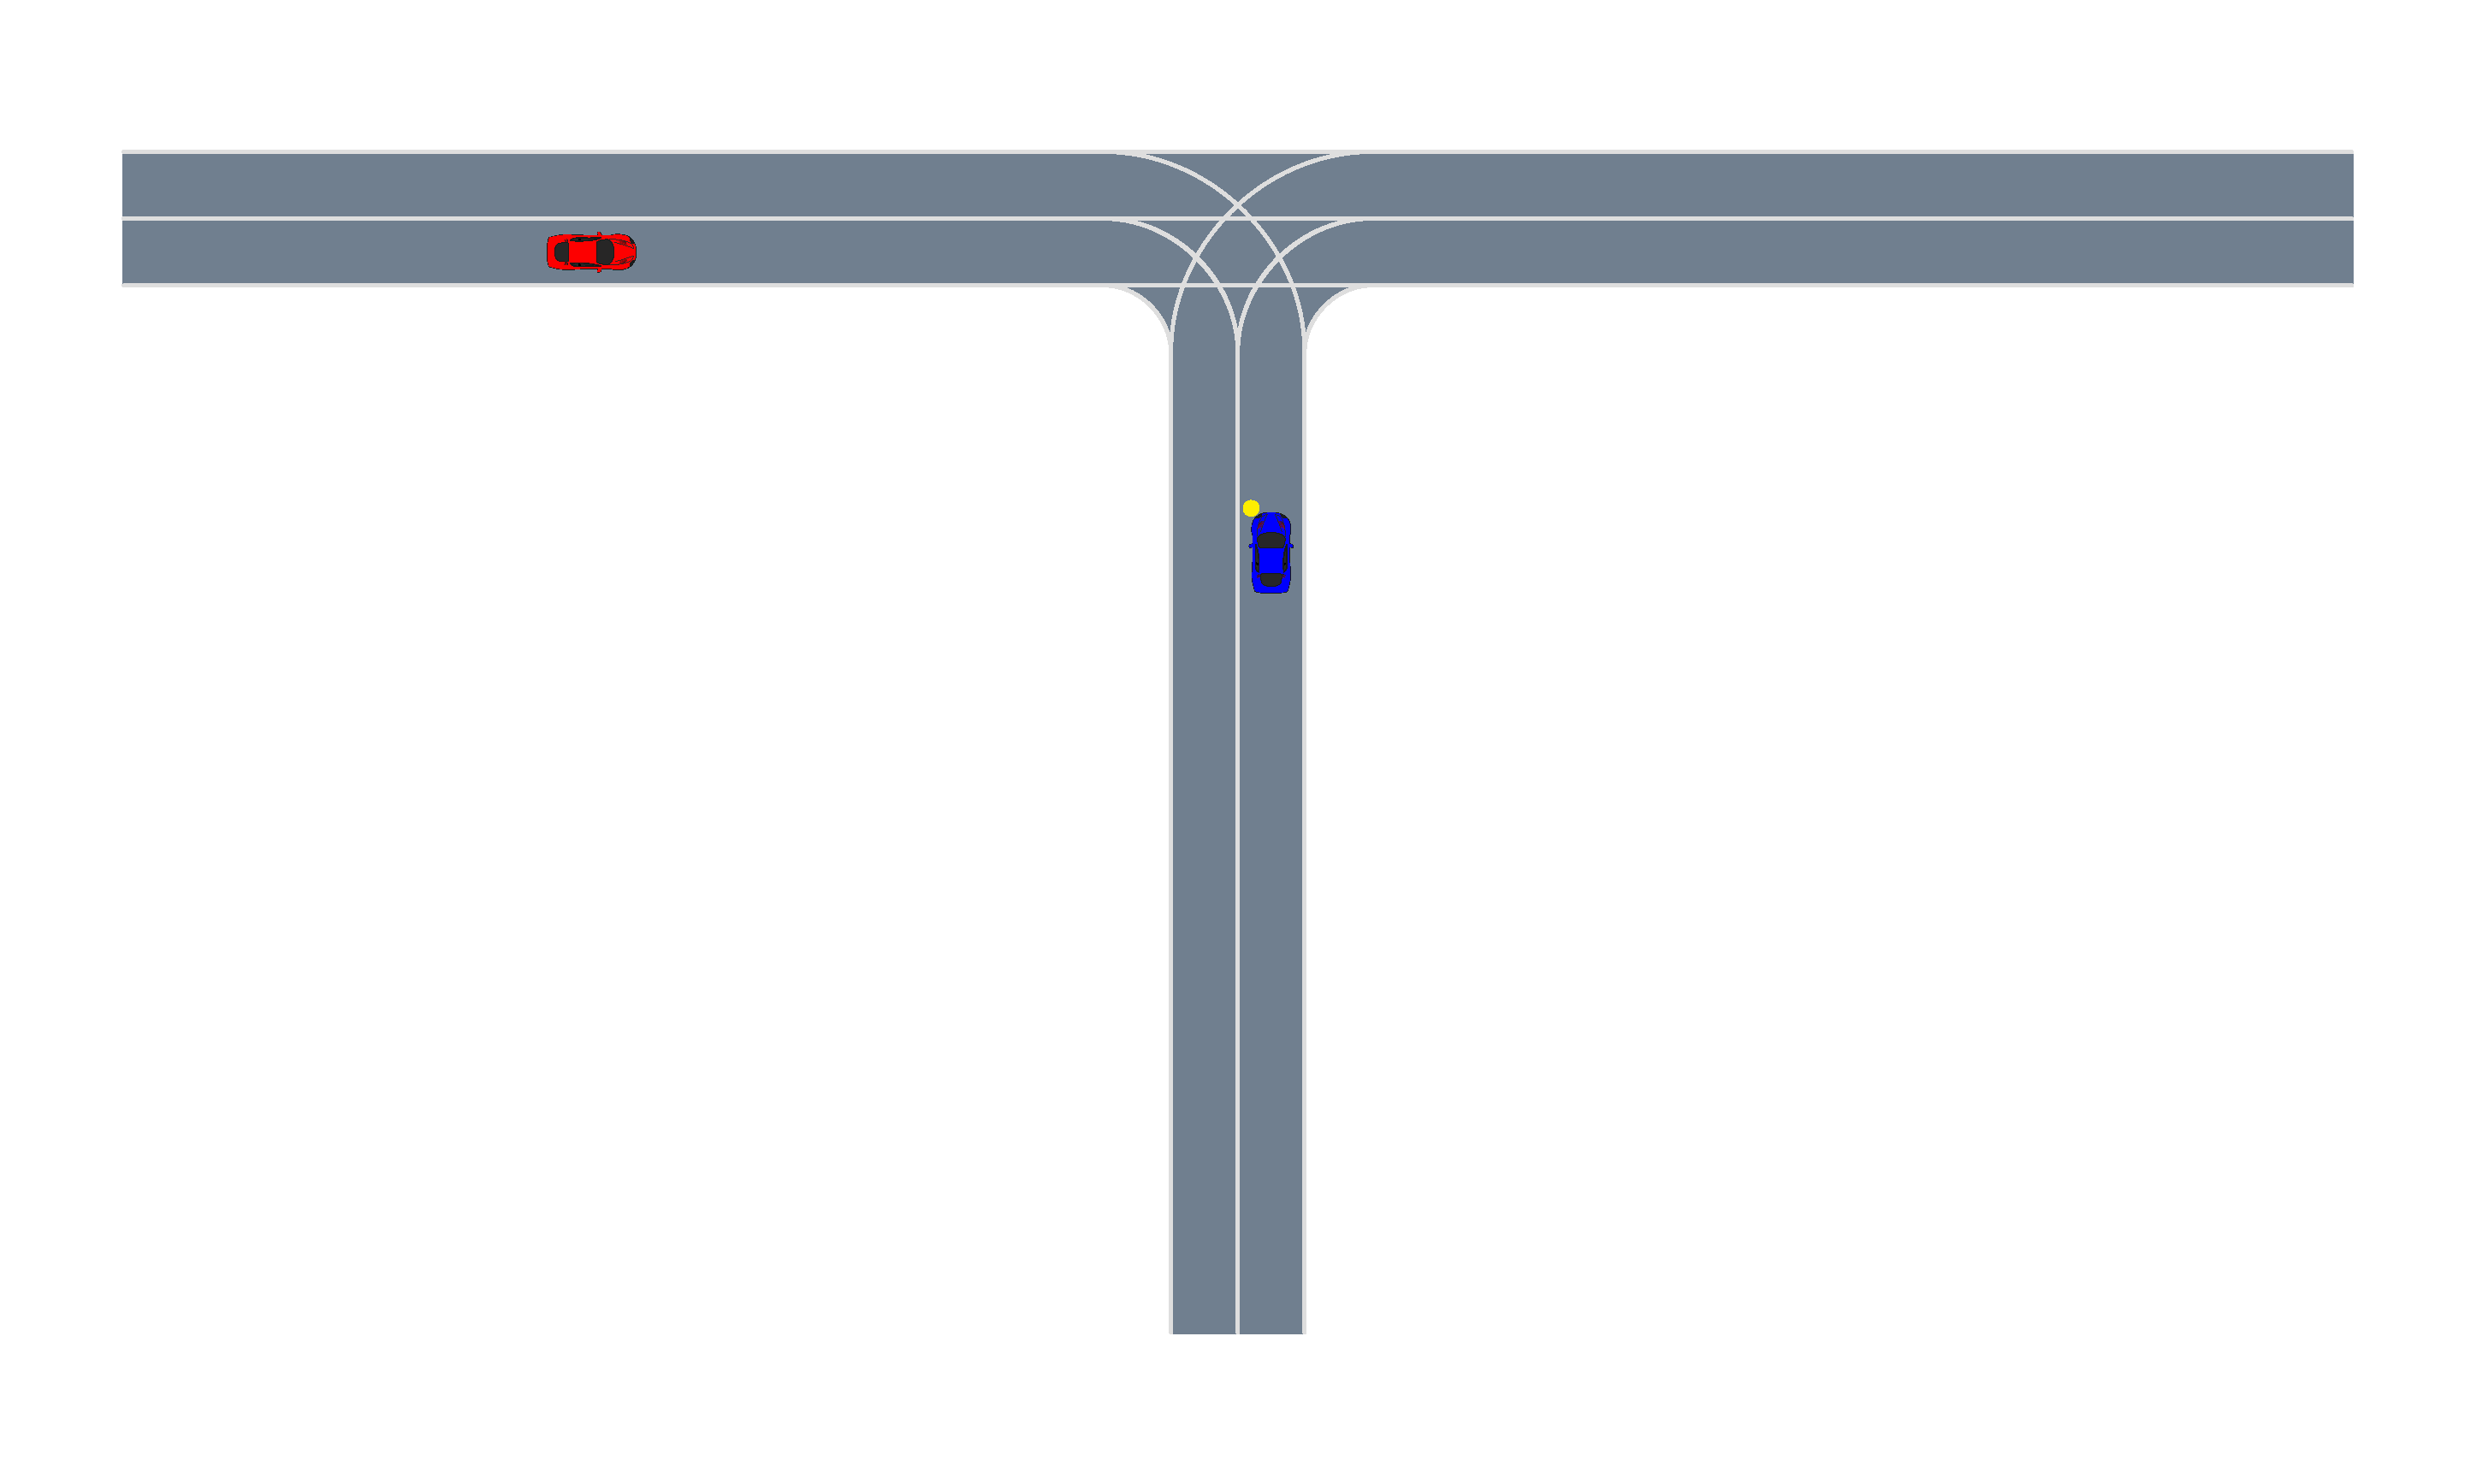
\includegraphics[width=0.9\textwidth, trim={10cm 16.5cm 22cm 0},clip]{figures/interpretable_validation/2car_res1_frame_01.pdf}
    \end{subfigure}%
   \begin{subfigure}[t]{0.33\columnwidth}
        \centering
        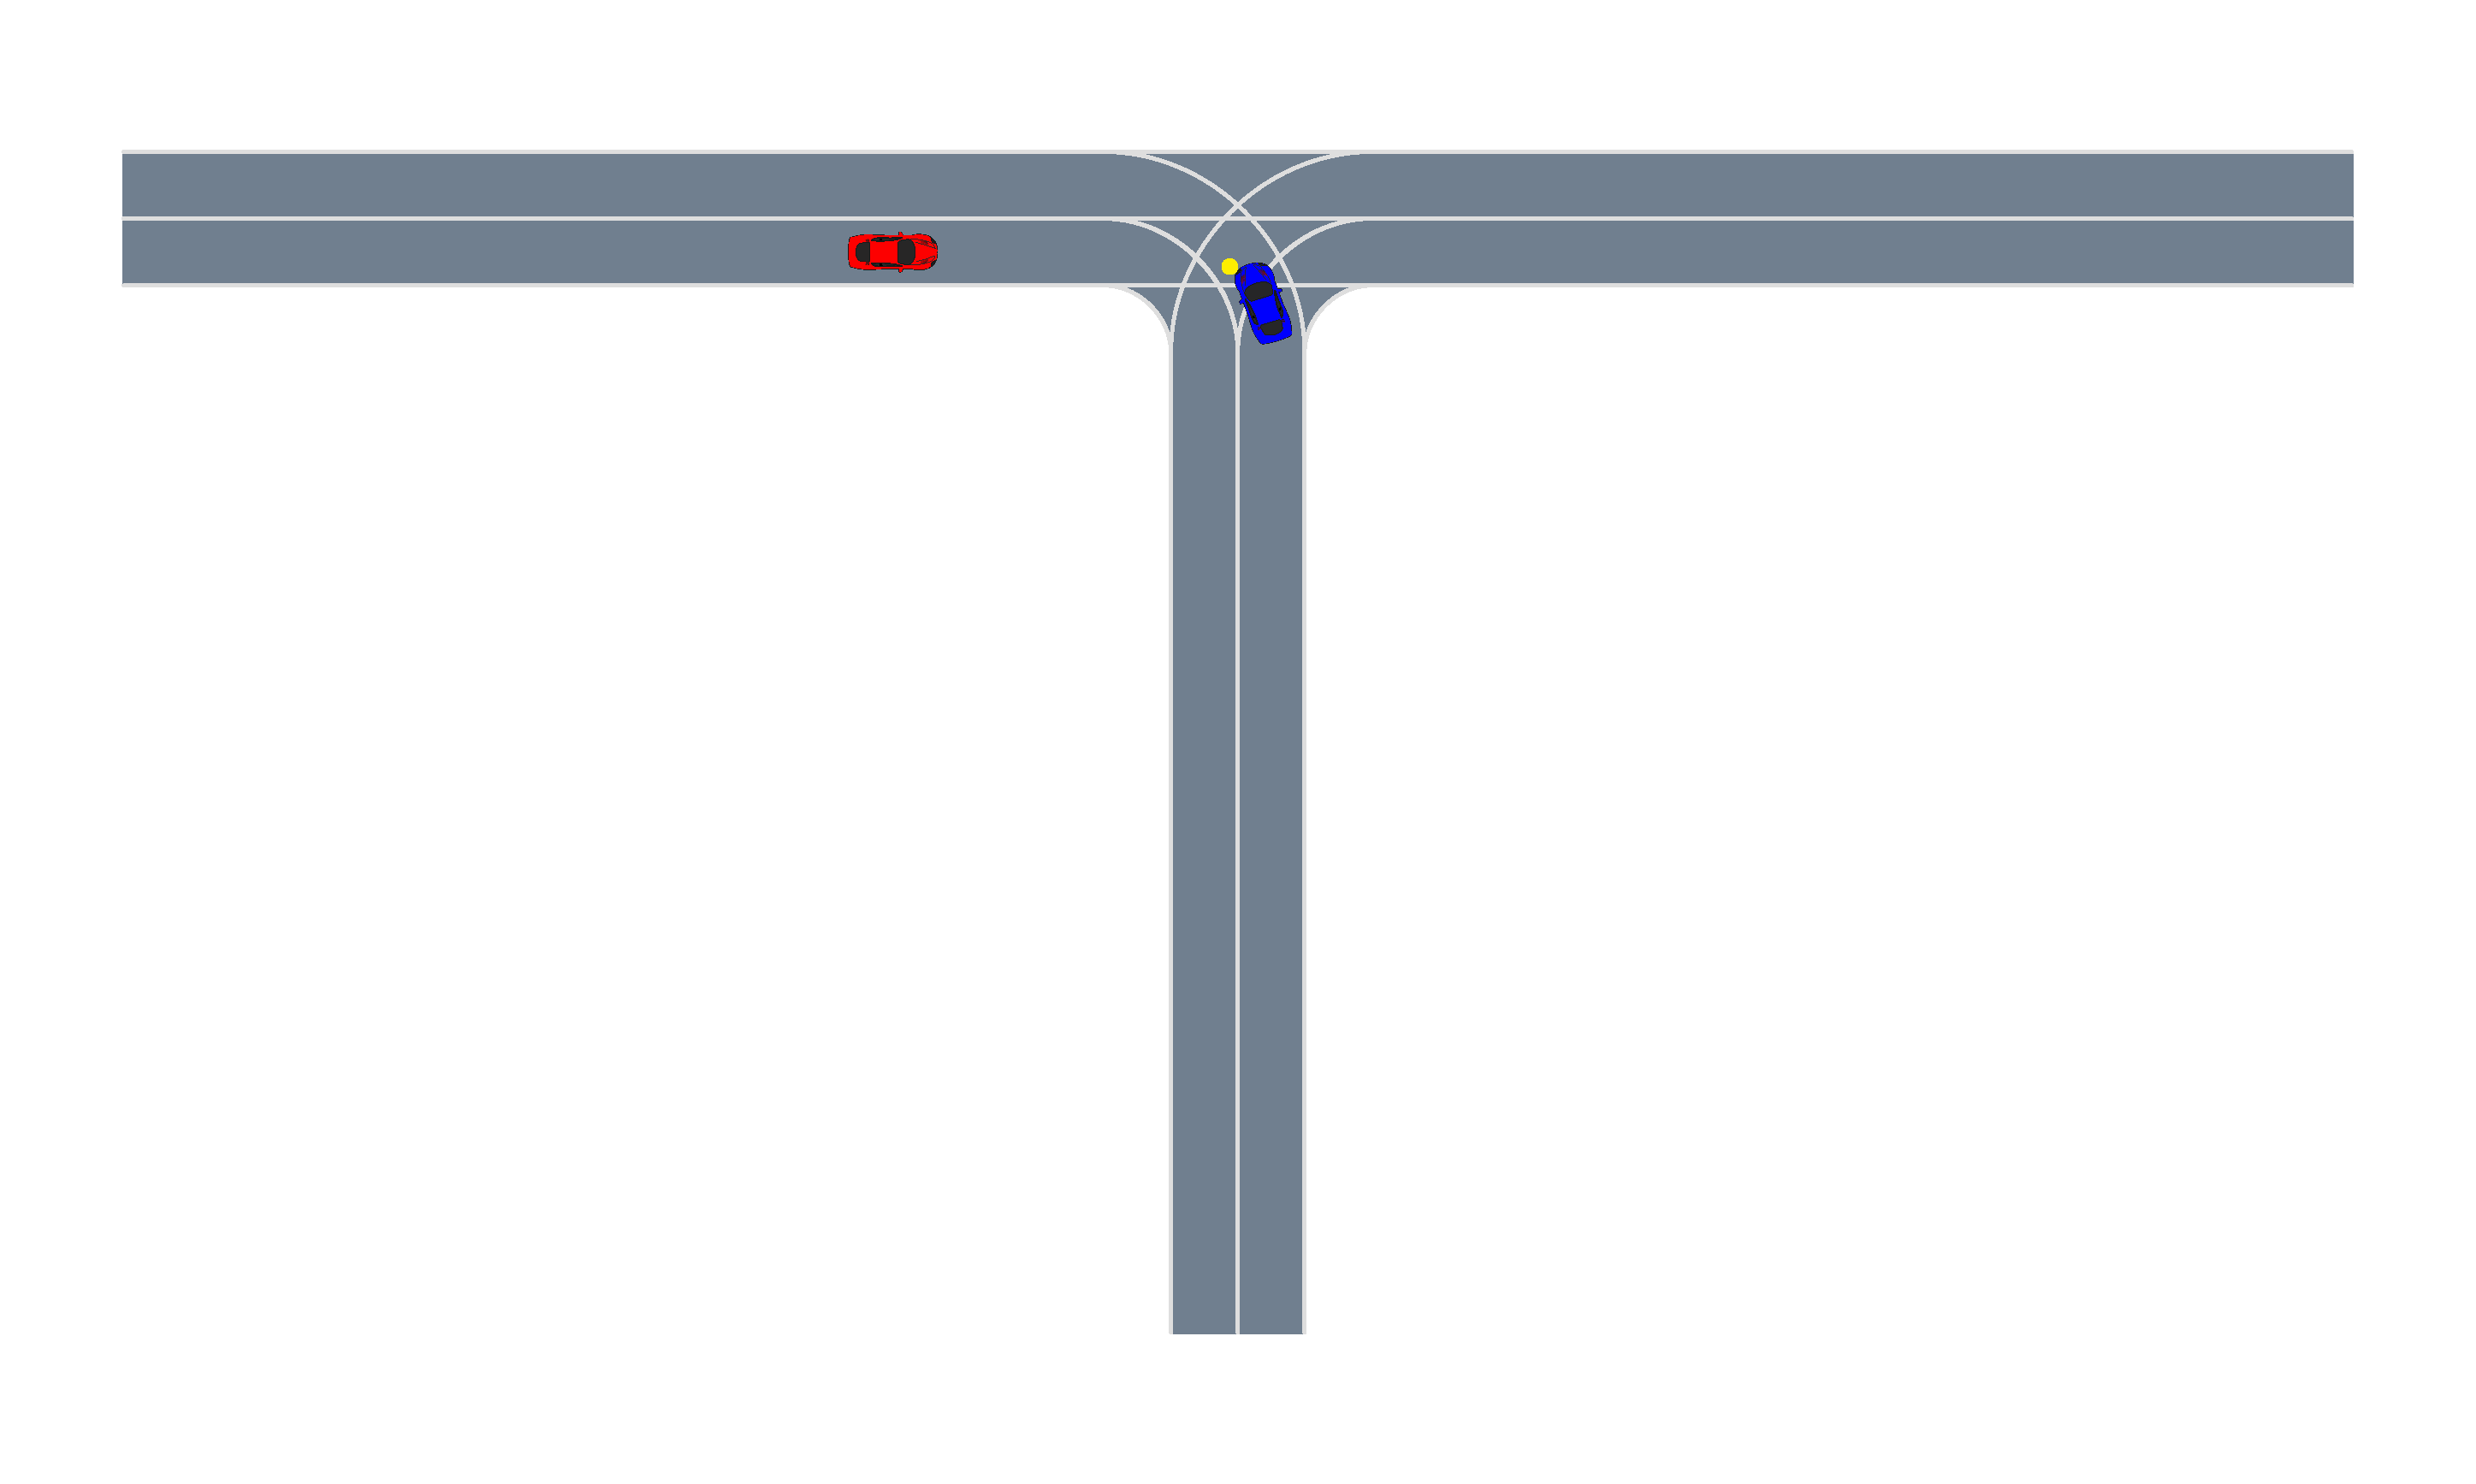
\includegraphics[width=0.9\textwidth, trim={10cm 16.5cm 22cm 0},clip]{figures/interpretable_validation/2car_res1_frame_07.pdf}
    \end{subfigure}%
    \begin{subfigure}[t]{0.33\columnwidth}
        \centering
        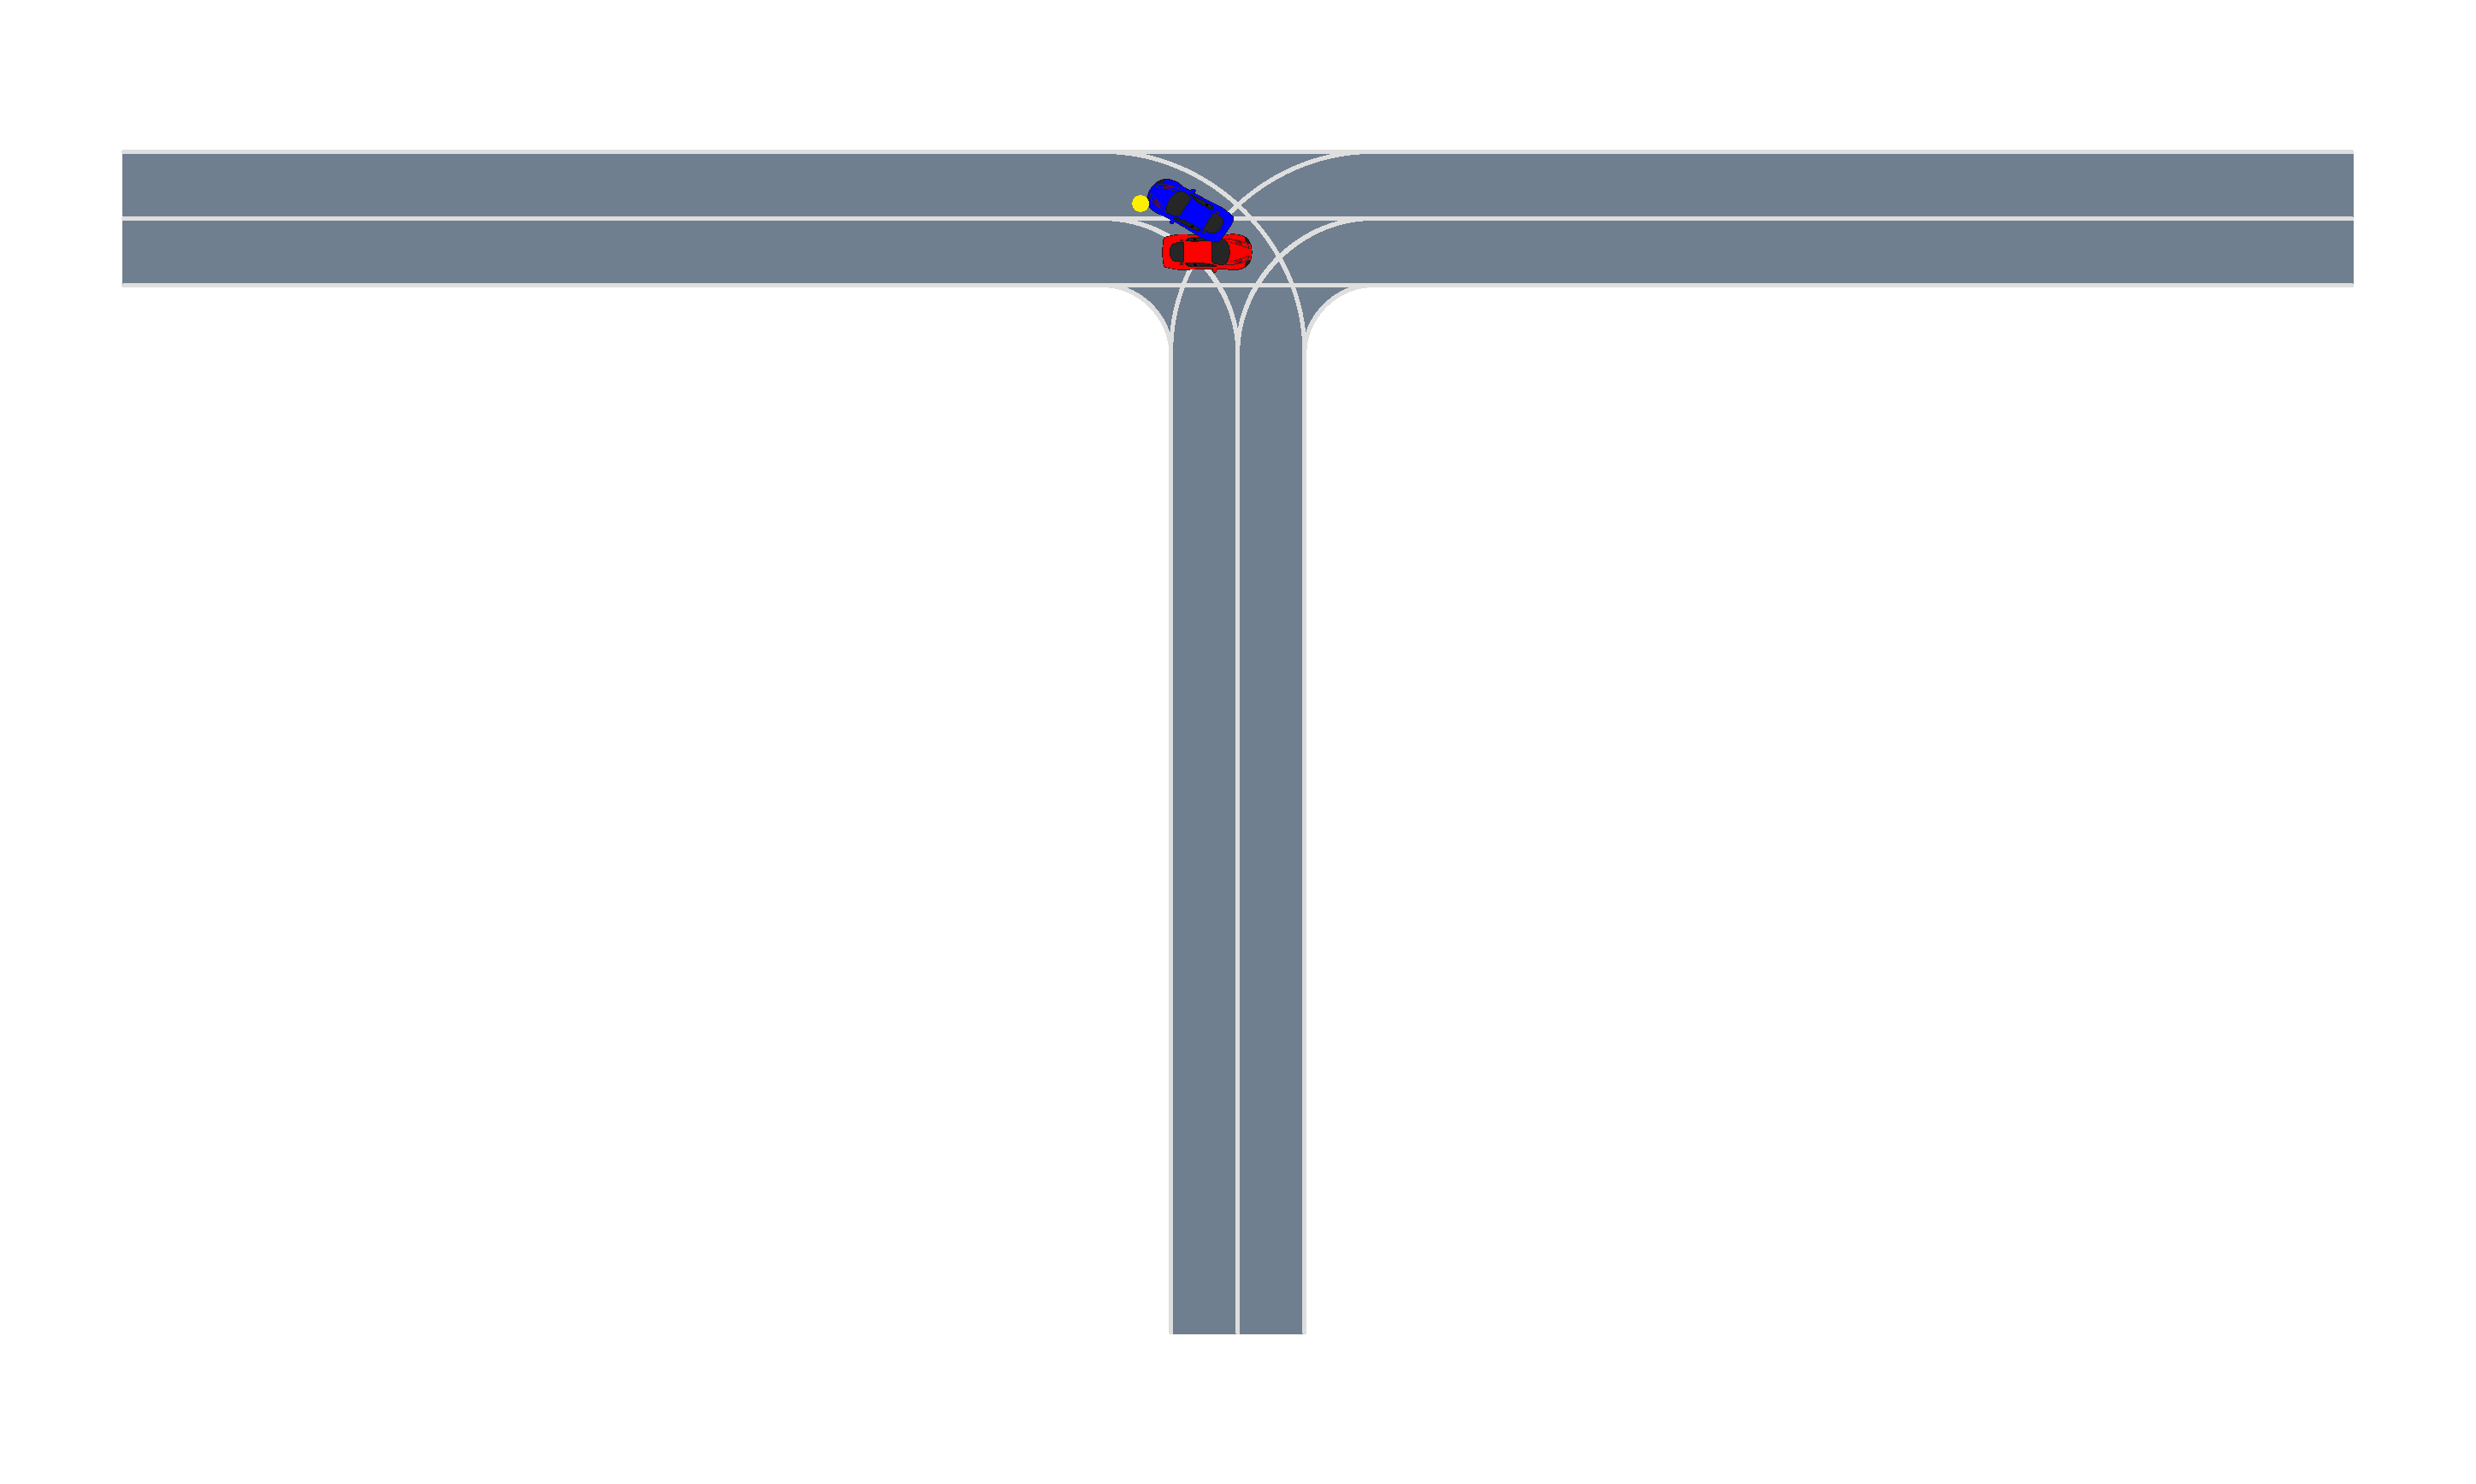
\includegraphics[width=0.9\textwidth, trim={10cm 16.5cm 22cm 0},clip]{figures/interpretable_validation/2car_res1_frame_12.pdf}
    \end{subfigure}
    \caption{Collision for LT1 at $t=(\SI{0}{s}, \SI{1.08}{s}, \SI{1.98}{s})$.}
    \label{fig:2car_LT1}
\end{figure}


%%%% Second initial condition
\begin{figure}
    \centering
    \begin{subfigure}[t]{0.33\columnwidth}
        \centering
        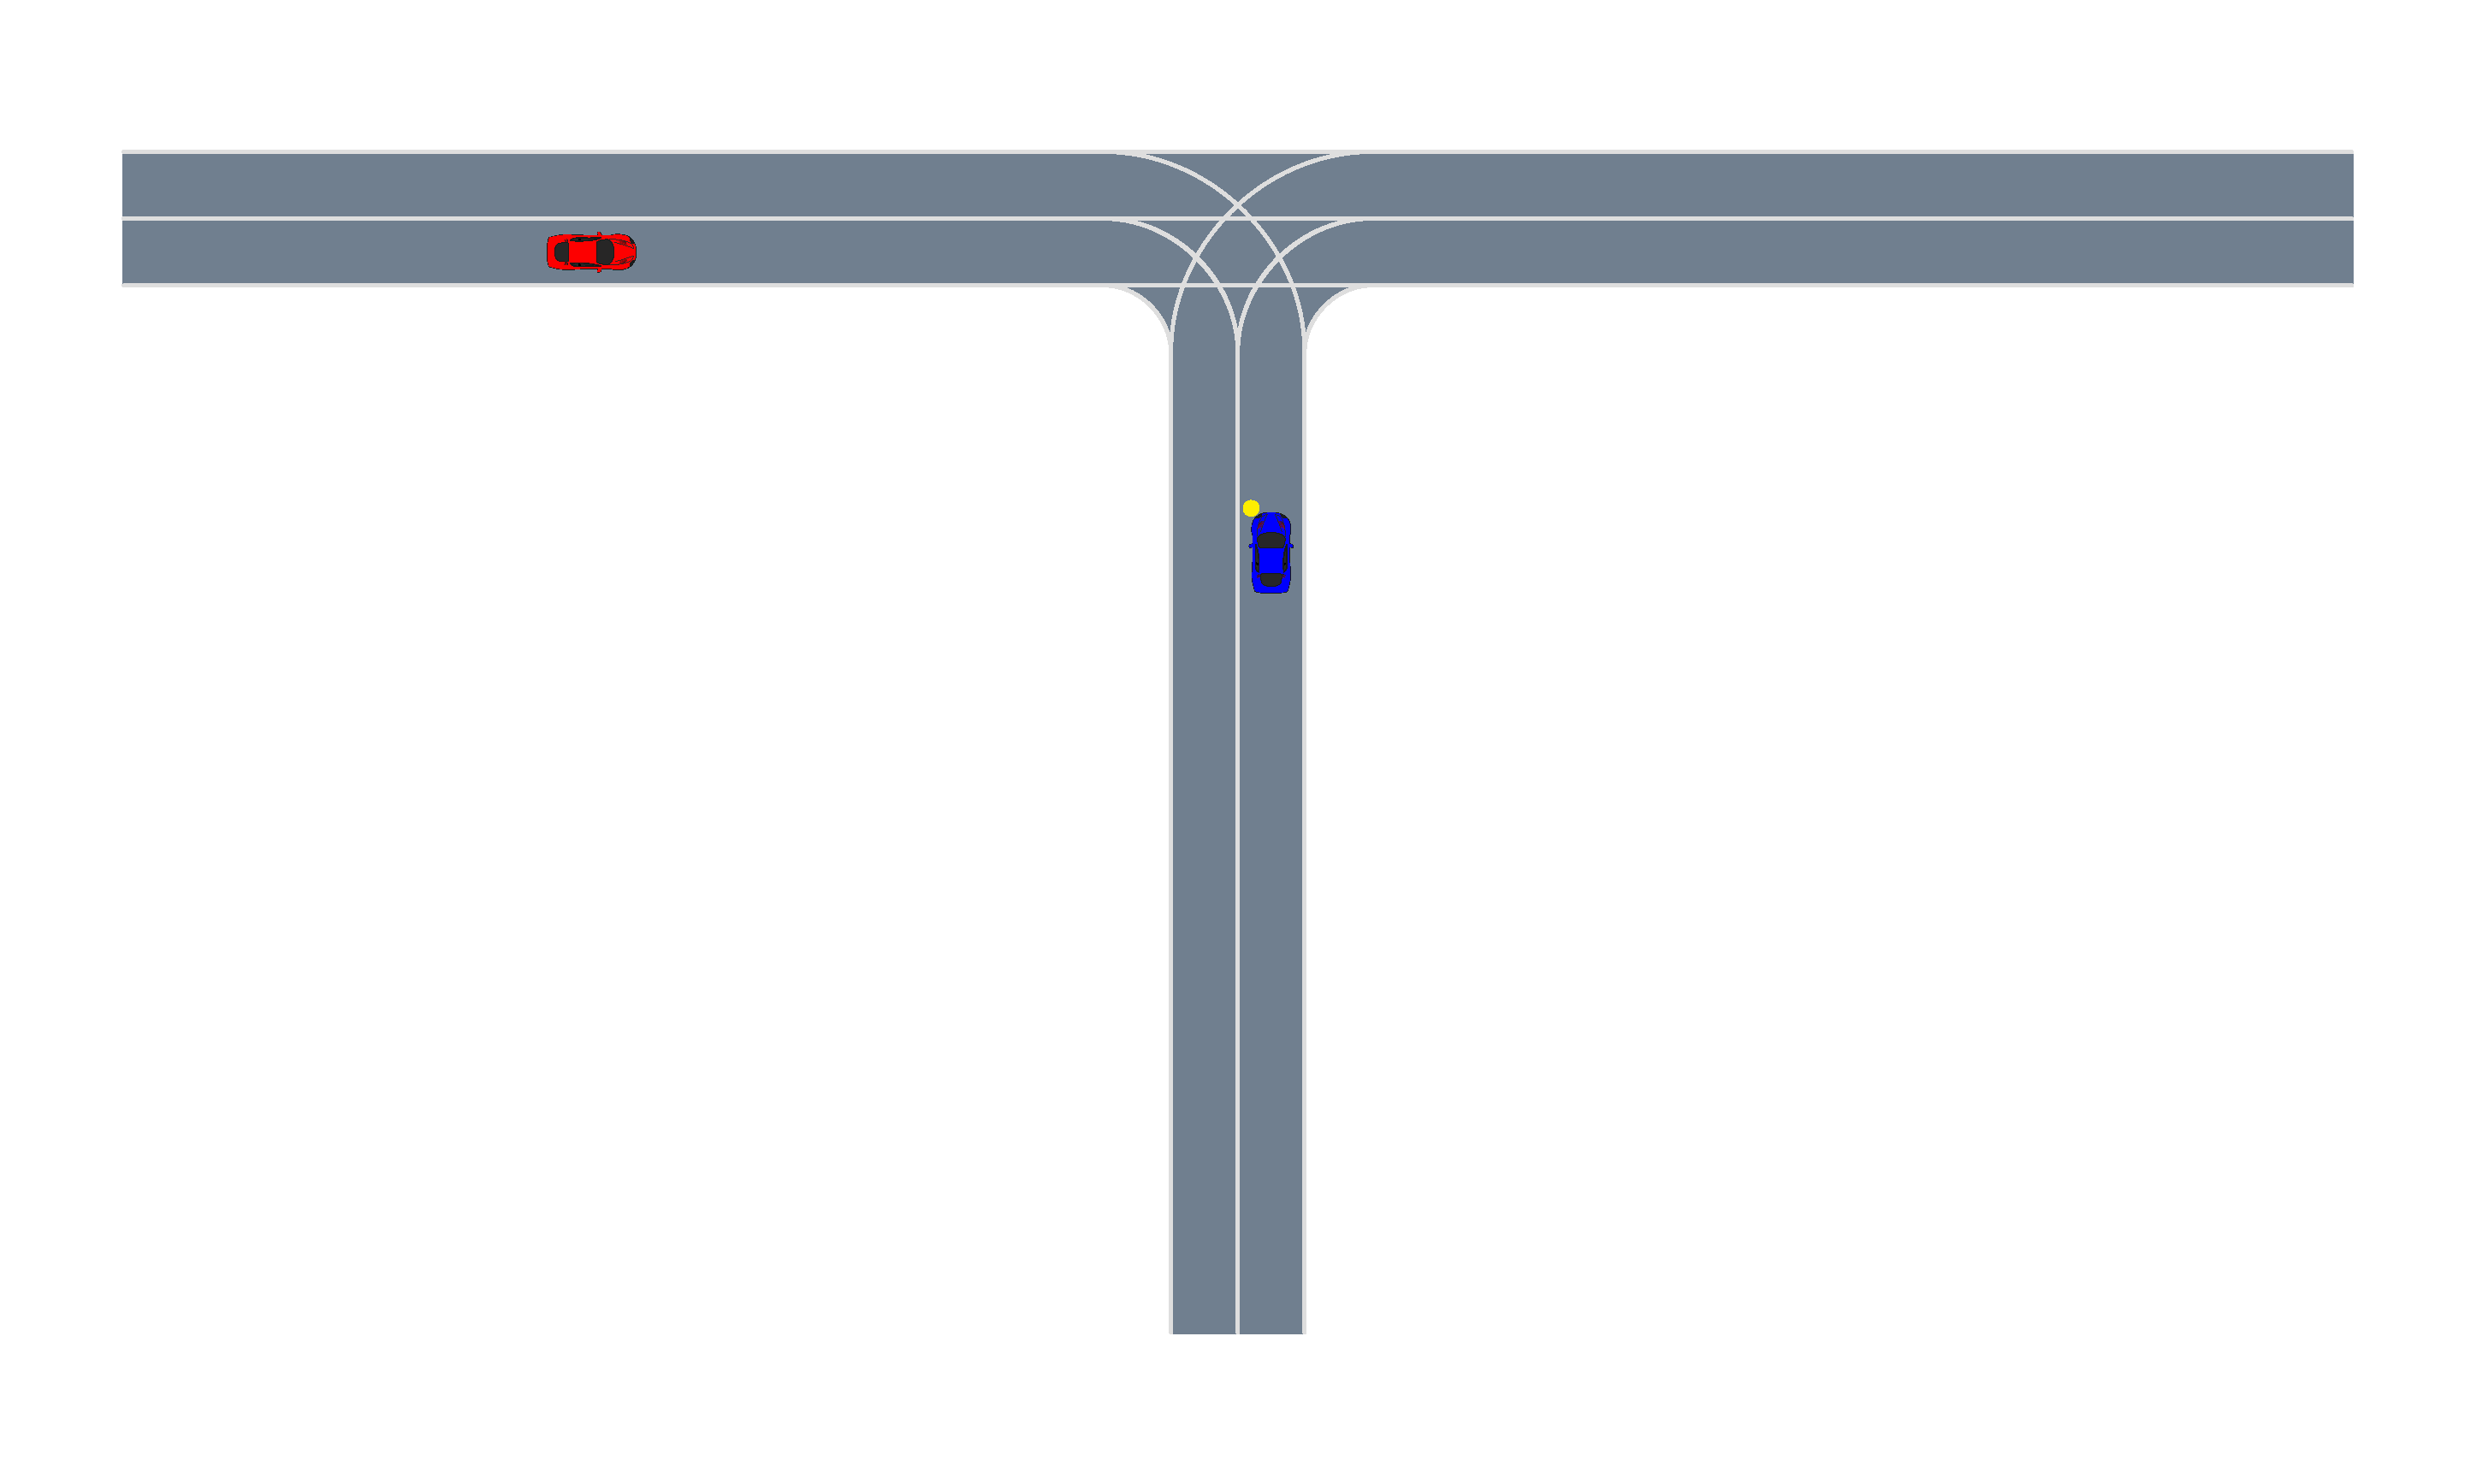
\includegraphics[width=0.9\textwidth, trim={10cm 16.5cm 22cm 0},clip]{figures/interpretable_validation/2car_res2_frame_01.pdf}
    \end{subfigure}%
   \begin{subfigure}[t]{0.33\columnwidth}
        \centering
        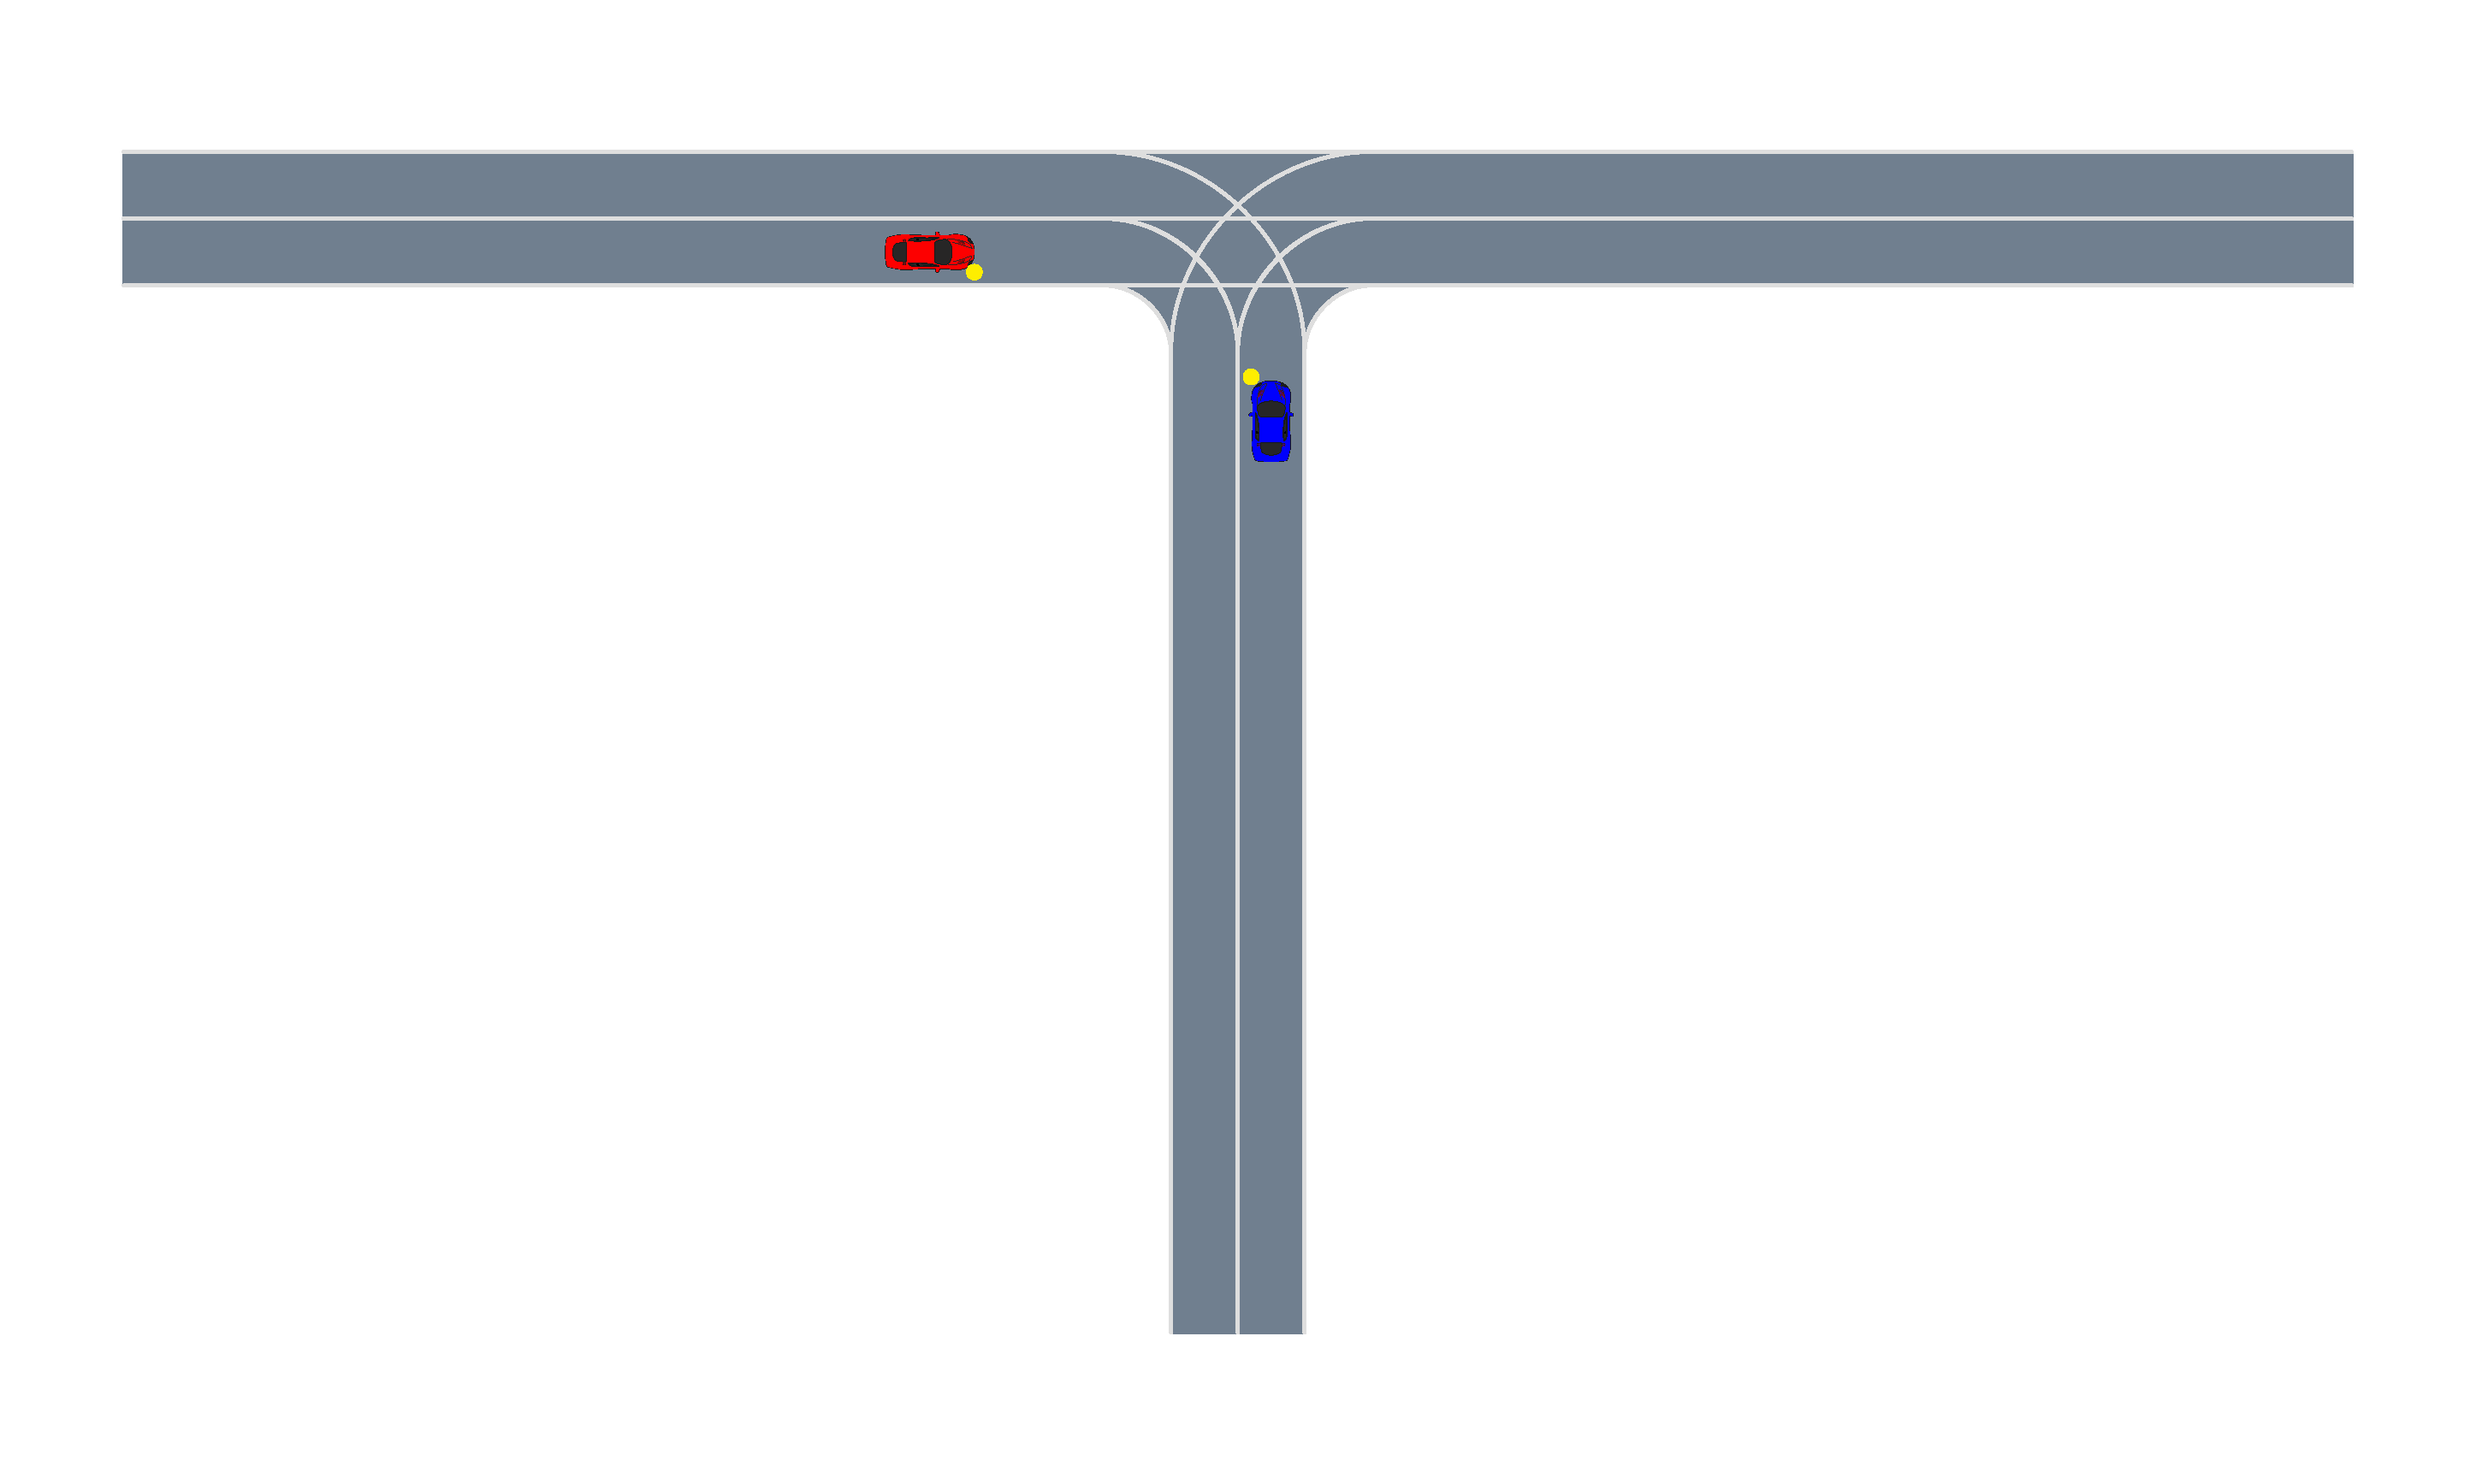
\includegraphics[width=0.9\textwidth, trim={10cm 16.5cm 22cm 0},clip]{figures/interpretable_validation/2car_res2_frame_05.pdf}
    \end{subfigure}%
    \begin{subfigure}[t]{0.33\columnwidth}
        \centering
        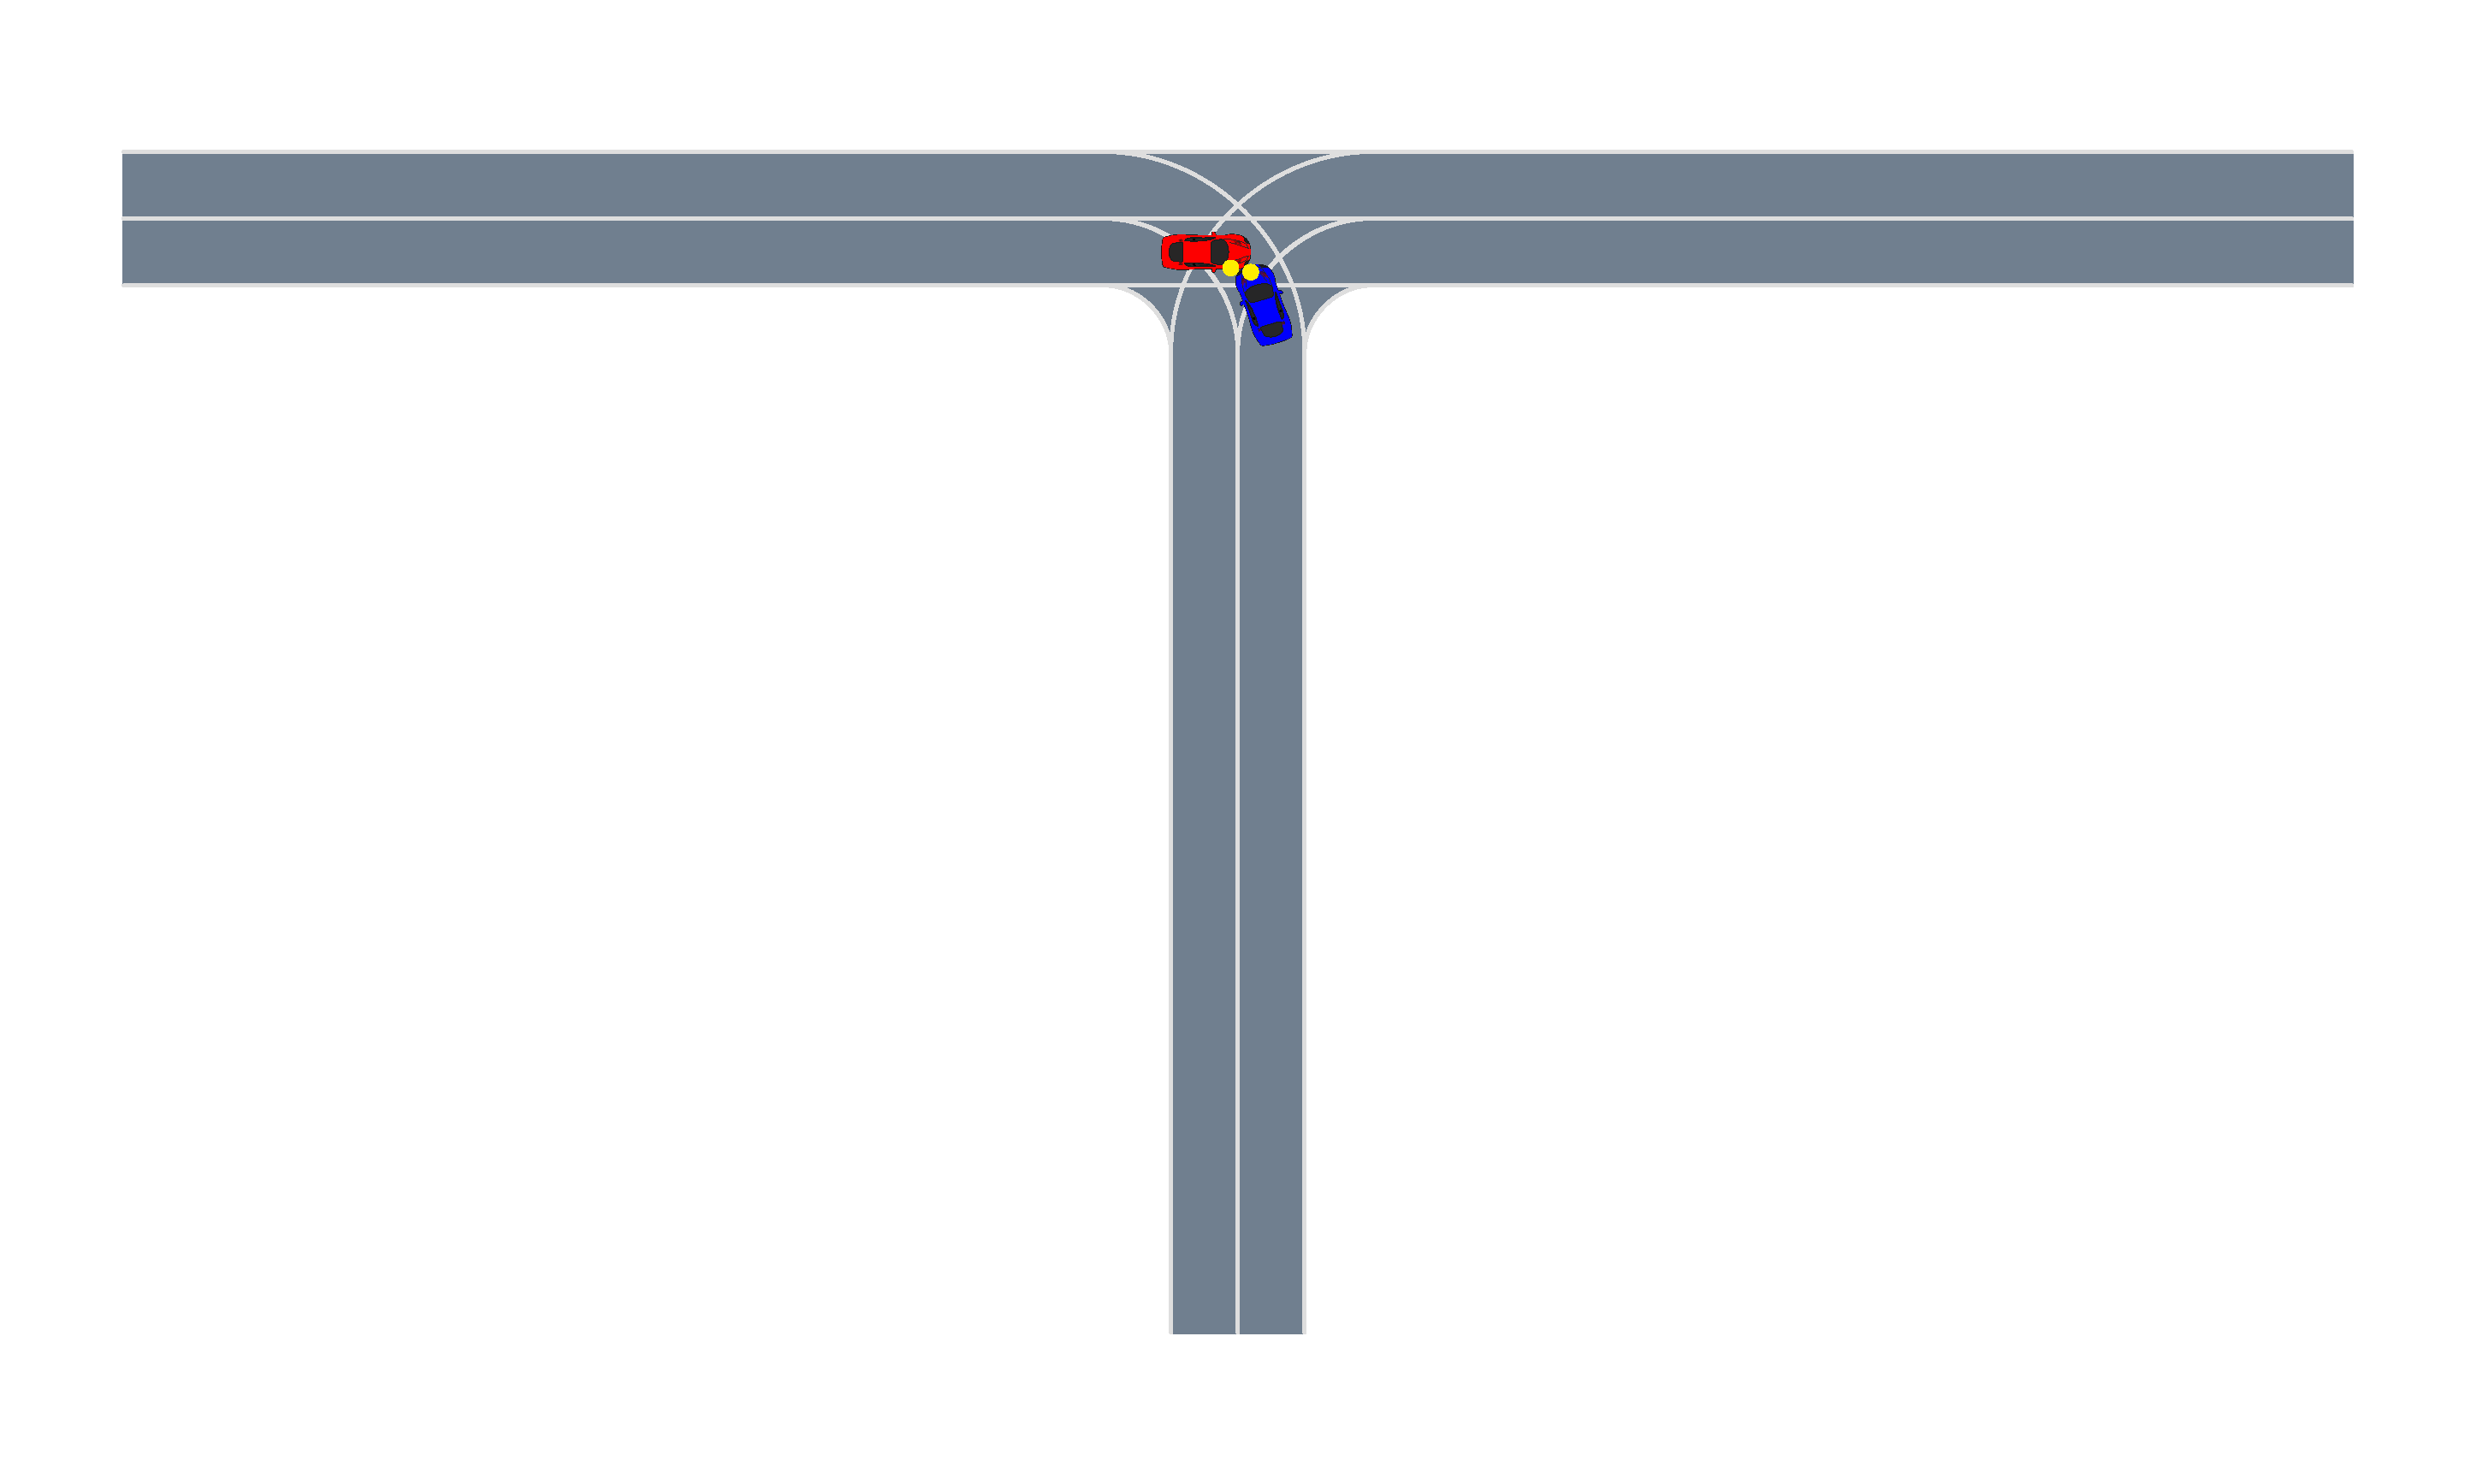
\includegraphics[width=0.9\textwidth, trim={10cm 16.5cm 22cm 0},clip]{figures/interpretable_validation/2car_res2_frame_08.pdf}
    \end{subfigure}
    \caption{Collision for LT2 at $t=(\SI{0}{s}, \SI{0.72}{s}, \SI{1.26}{s})$.}
    \label{fig:2car_LT2}
\end{figure}


%%% Third initial condition
\begin{figure}
    \centering
    \begin{subfigure}[t]{0.33\columnwidth}
        \centering
        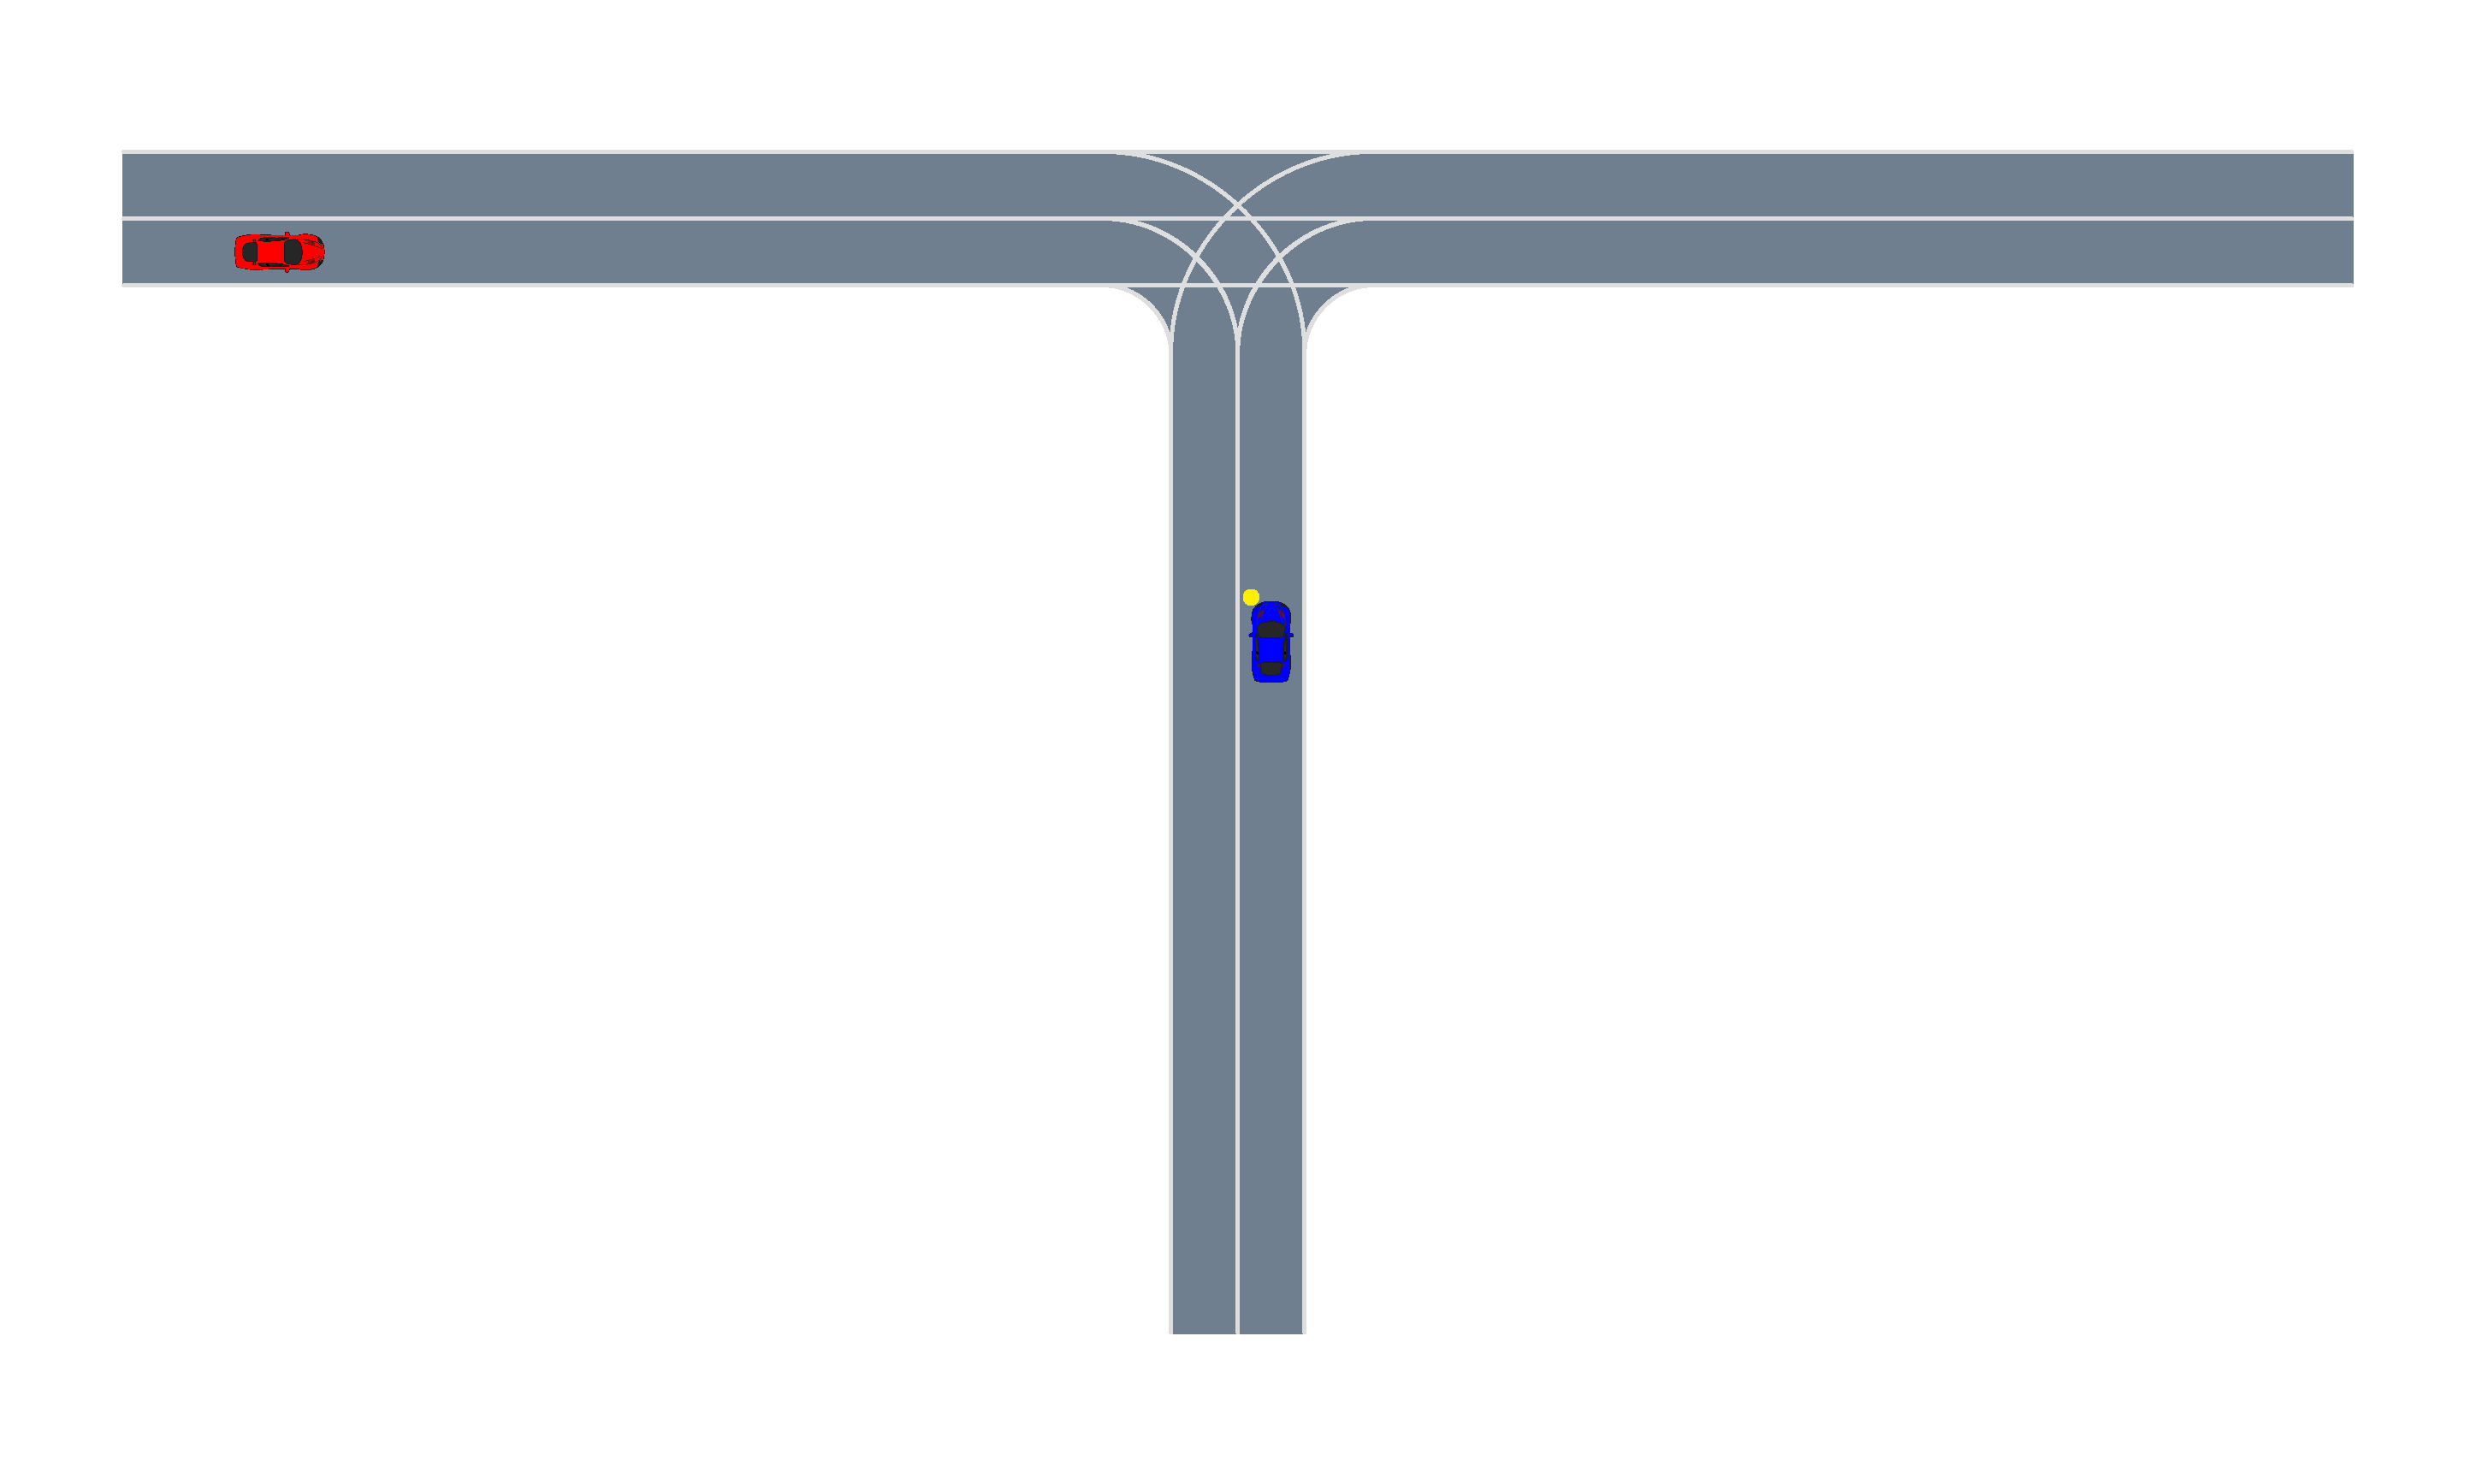
\includegraphics[width=0.9\textwidth, trim={8cm 16cm 22cm 0},clip]{figures/interpretable_validation/2car_res3_frame_01.pdf}
    \end{subfigure}%
   \begin{subfigure}[t]{0.33\columnwidth}
        \centering
        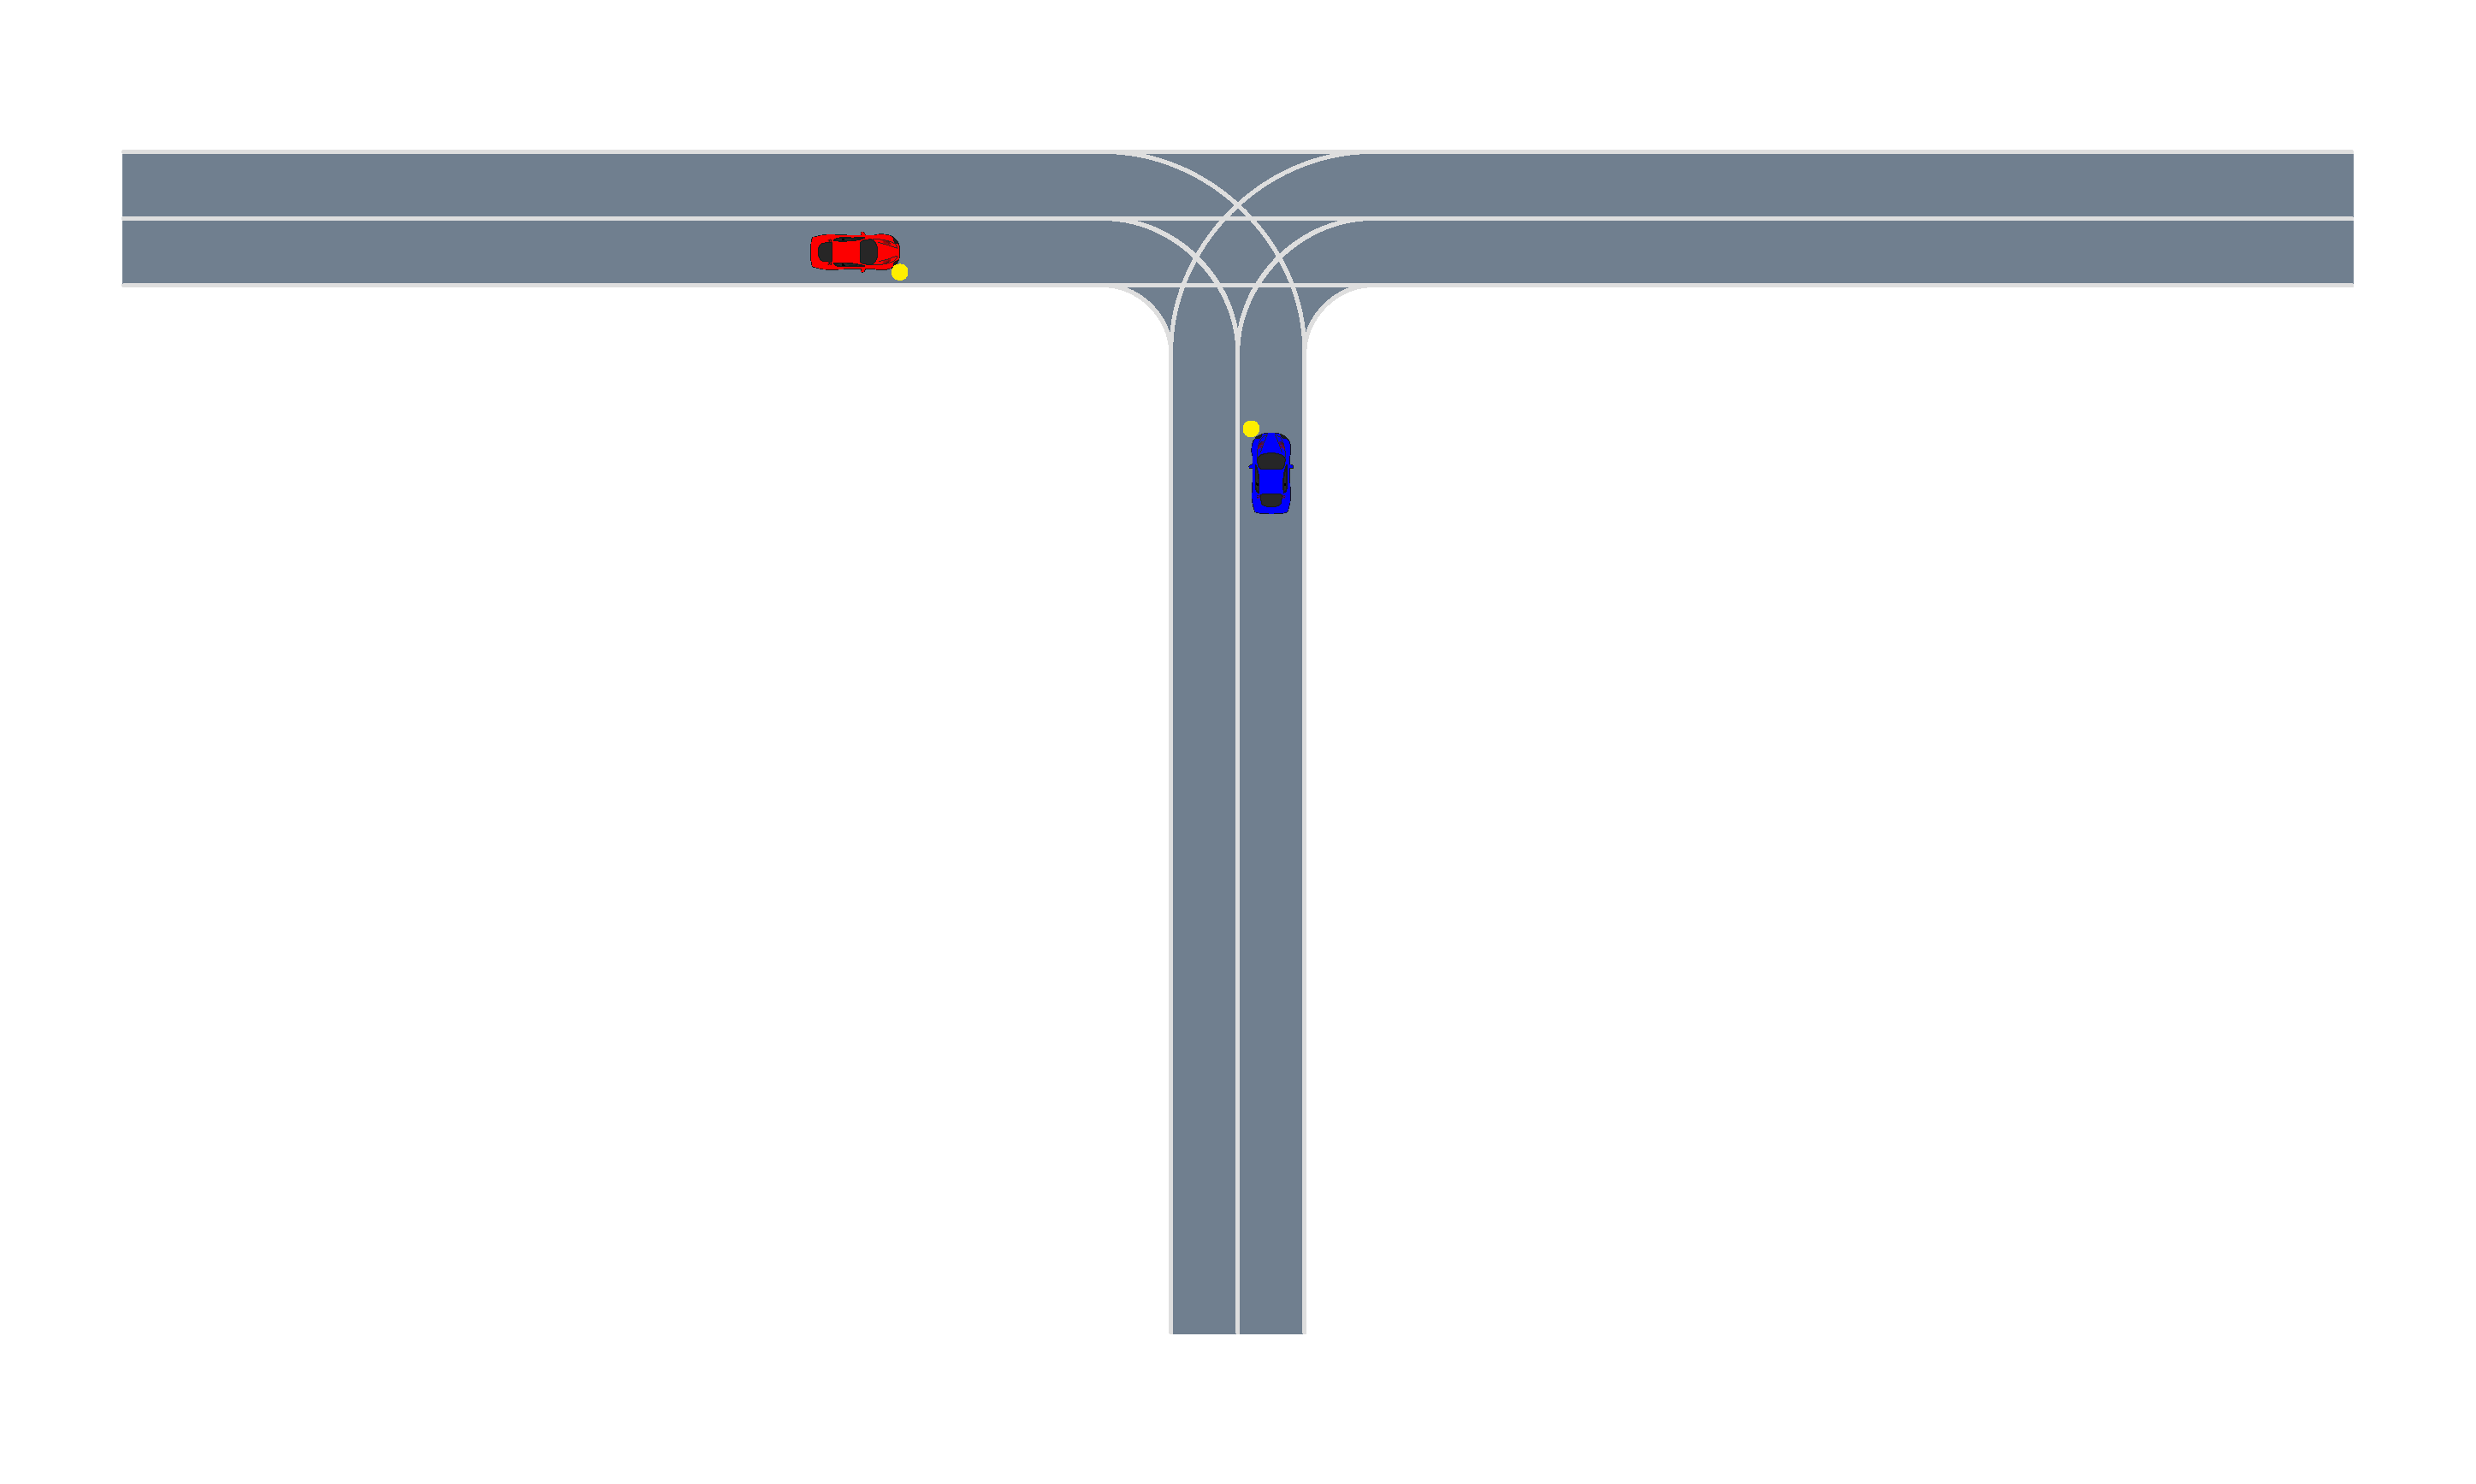
\includegraphics[width=0.9\textwidth, trim={10cm 16.5cm 22cm 0},clip]{figures/interpretable_validation/2car_res3_frame_06.pdf}
    \end{subfigure}%
    \begin{subfigure}[t]{0.33\columnwidth}
        \centering
        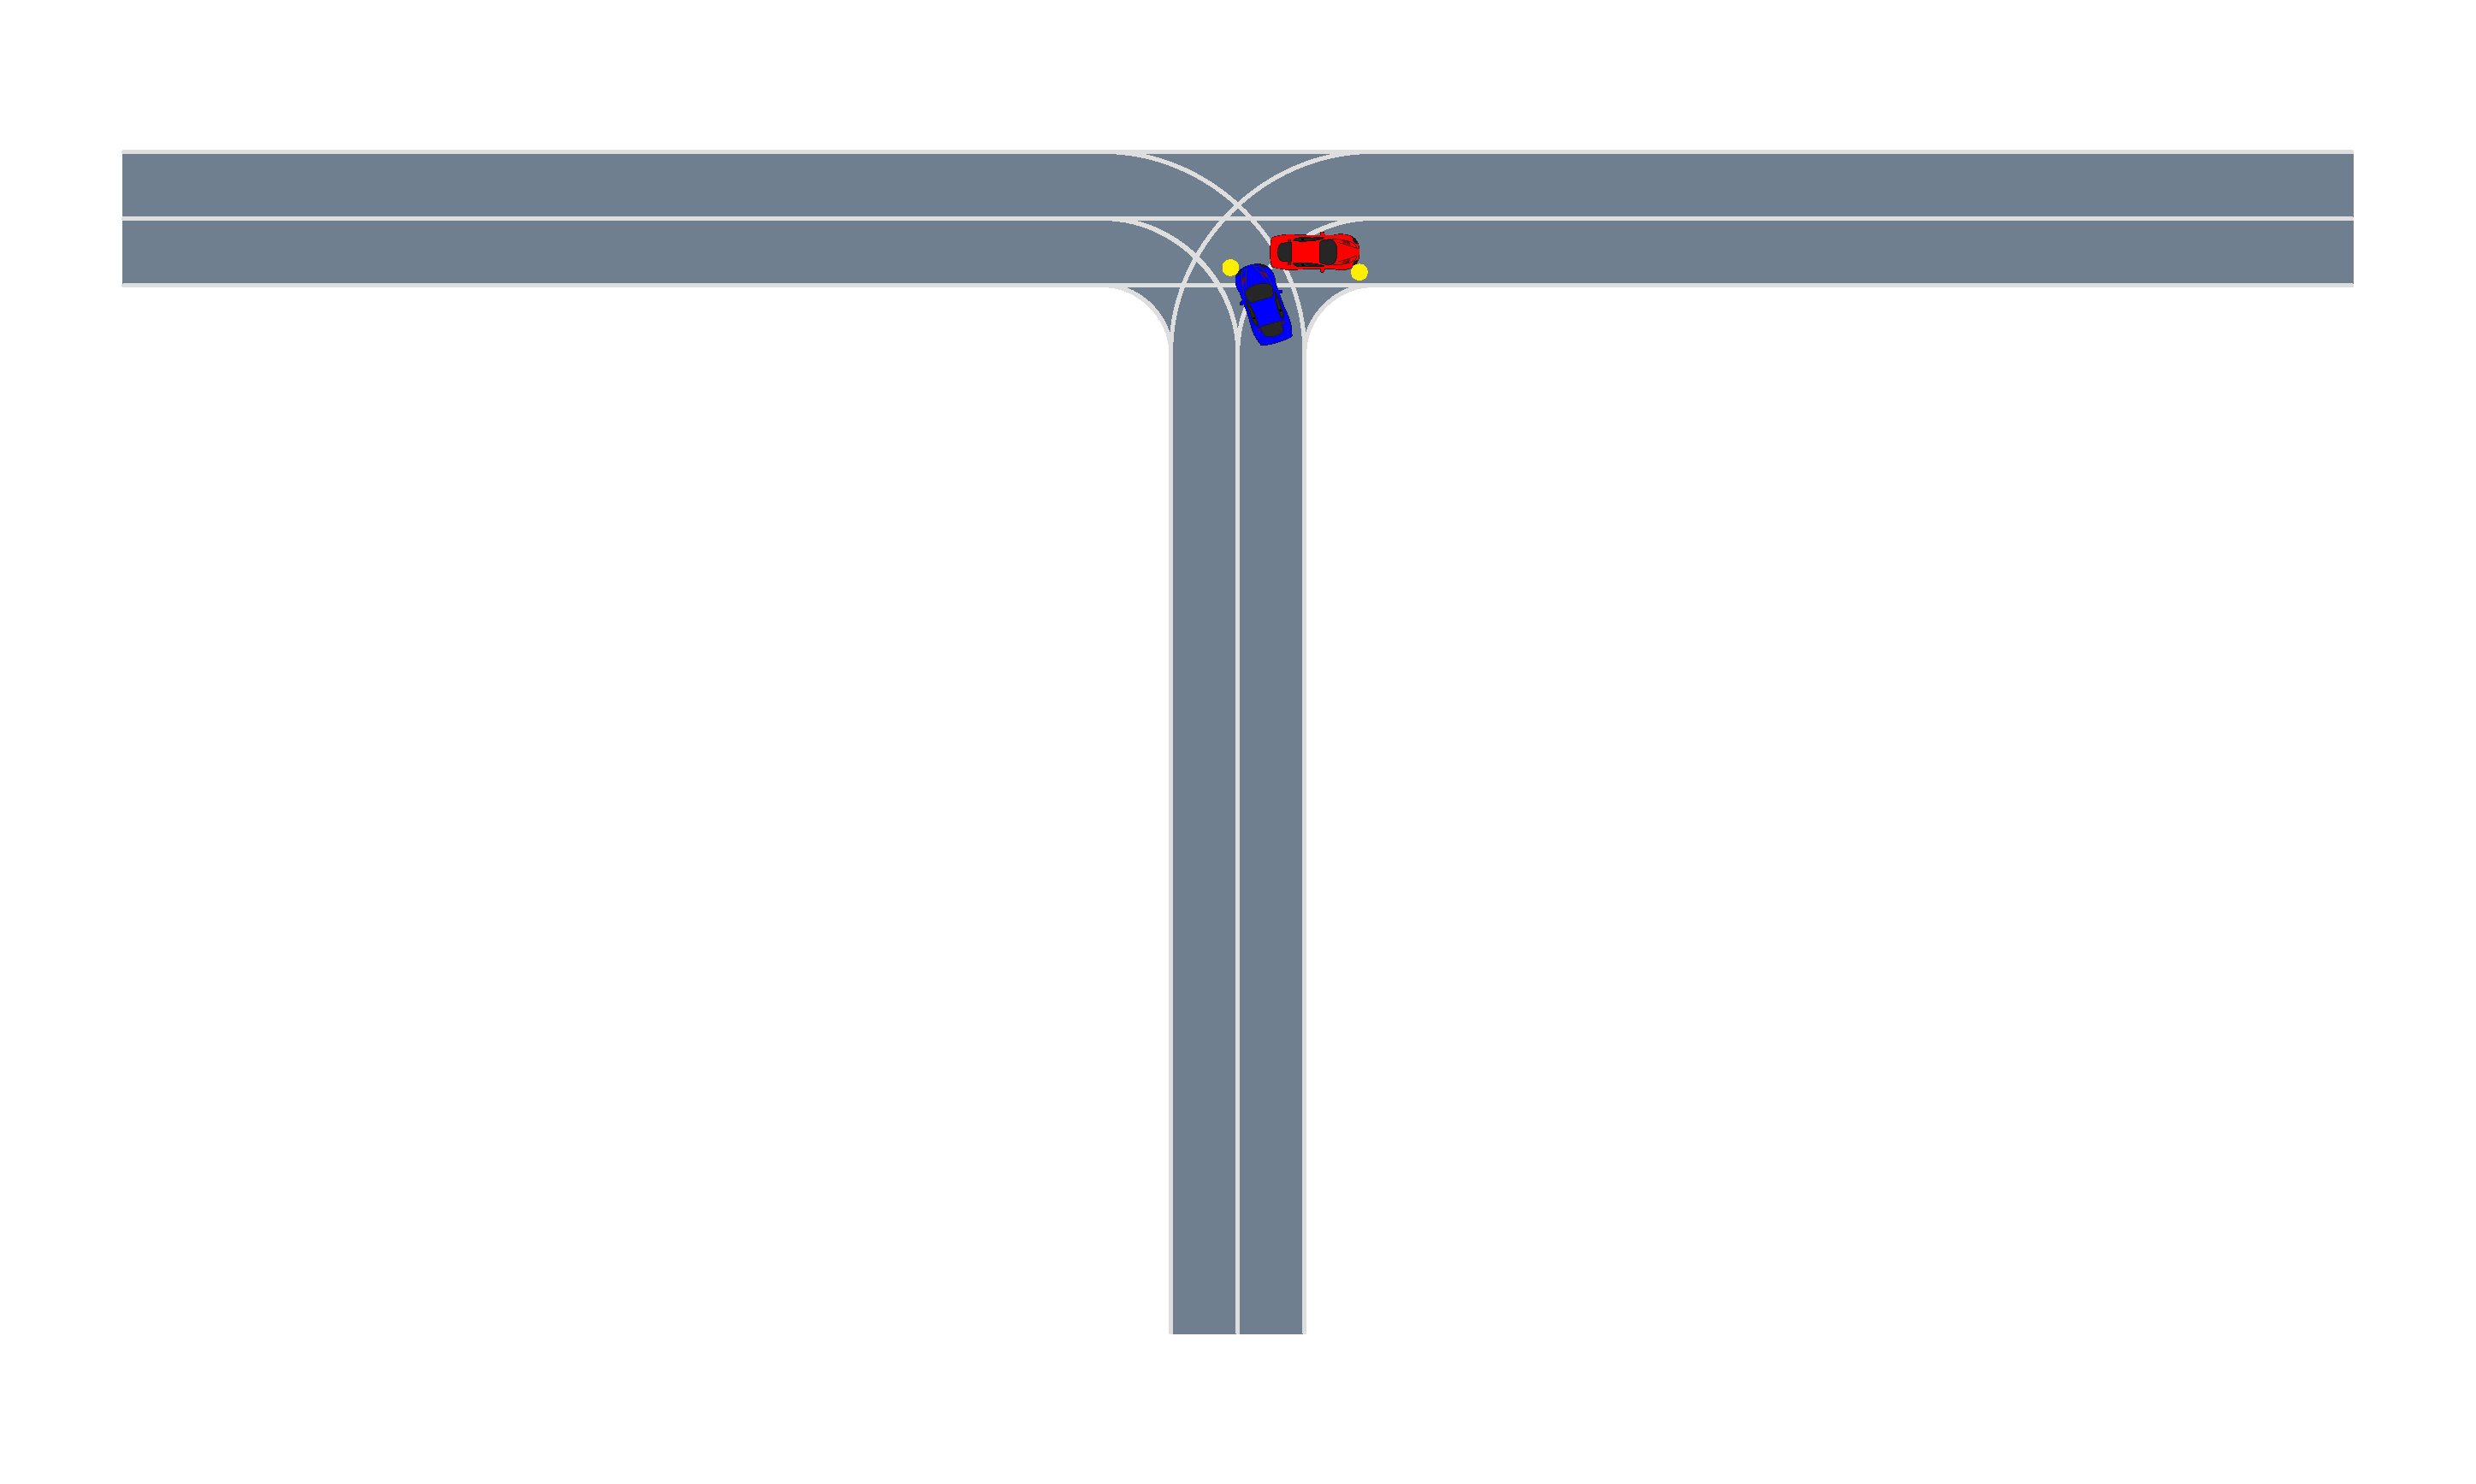
\includegraphics[width=0.9\textwidth, trim={10cm 16.5cm 22cm 0},clip]{figures/interpretable_validation/2car_res3_frame_10.pdf}
    \end{subfigure}
    \caption{Collision for LT3 at $t=(\SI{0}{s}, \SI{0.90}{s}, \SI{1.62}{s})$.}
    \label{fig:2car_LT3}
\end{figure}

% Sampling failure examples
One benefit to learning a failure description is the ability to produce many failure examples that have a shared temporal property. For example, we took the third failure description
\begin{equation}
    \square_{[0, .36]} B \lor d_{\rm maj}
\end{equation}
and use it to sample \num{10} failure trajectores. We plot the velocity vs. the position of the adversary for the failure examples in \cref{fig:2car_failure_samples}. We see that in the first two timesteps there is always a signification slowdown, but the trajectories then evolve stochastically before ending in a failure. 

\begin{figure}
    \centering
    \begin{tikzpicture}[/tikz/background rectangle/.style={fill={rgb,1:red,1.0;green,1.0;blue,1.0}, draw opacity={1.0}}, show background rectangle]
\begin{axis}[point meta max={nan}, point meta min={nan}, legend cell align={left}, title={Failure Examples}, title style={at={{(0.5,1)}}, anchor={south}, font={{\fontsize{14 pt}{18.2 pt}\selectfont}}, color={rgb,1:red,0.0;green,0.0;blue,0.0}, draw opacity={1.0}, rotate={0.0}}, legend style={color={rgb,1:red,0.0;green,0.0;blue,0.0}, draw opacity={1.0}, line width={1}, solid, fill={rgb,1:red,1.0;green,1.0;blue,1.0}, fill opacity={1.0}, text opacity={1.0}, font={{\fontsize{8 pt}{10.4 pt}\selectfont}}, at={(0.98, 0.98)}, anchor={north east}}, axis background/.style={fill={rgb,1:red,1.0;green,1.0;blue,1.0}, opacity={1.0}}, anchor={north west}, xshift={1.0mm}, yshift={-1.0mm}, width={0.9\textwidth}, height={75mm}, scaled x ticks={false}, xlabel={Position (m)}, x tick style={color={rgb,1:red,0.0;green,0.0;blue,0.0}, opacity={1.0}}, x tick label style={color={rgb,1:red,0.0;green,0.0;blue,0.0}, opacity={1.0}, rotate={0}}, xlabel style={at={(ticklabel cs:0.5)}, anchor=near ticklabel, font={{\fontsize{11 pt}{14.3 pt}\selectfont}}, color={rgb,1:red,0.0;green,0.0;blue,0.0}, draw opacity={1.0}, rotate={0.0}}, xmajorgrids={true}, xmin={13.987323701839703}, xmax={49.768552903503526}, xtick={{15.0,20.0,25.0,30.0,35.0,40.0,45.0}}, xticklabels={{$15$,$20$,$25$,$30$,$35$,$40$,$45$}}, xtick align={inside}, xticklabel style={font={{\fontsize{8 pt}{10.4 pt}\selectfont}}, color={rgb,1:red,0.0;green,0.0;blue,0.0}, draw opacity={1.0}, rotate={0.0}}, x grid style={color={rgb,1:red,0.0;green,0.0;blue,0.0}, draw opacity={0.1}, line width={0.5}, solid}, axis x line*={left}, x axis line style={color={rgb,1:red,0.0;green,0.0;blue,0.0}, draw opacity={1.0}, line width={1}, solid}, scaled y ticks={false}, ylabel={Velocity (m/s)}, y tick style={color={rgb,1:red,0.0;green,0.0;blue,0.0}, opacity={1.0}}, y tick label style={color={rgb,1:red,0.0;green,0.0;blue,0.0}, opacity={1.0}, rotate={0}}, ylabel style={at={(ticklabel cs:0.5)}, anchor=near ticklabel, font={{\fontsize{11 pt}{14.3 pt}\selectfont}}, color={rgb,1:red,0.0;green,0.0;blue,0.0}, draw opacity={1.0}, rotate={0.0}}, ymajorgrids={true}, ymin={14.291245239454959}, ymax={19.137148196909077}, ytick={{15.0,16.0,17.0,18.0,19.0}}, yticklabels={{$15$,$16$,$17$,$18$,$19$}}, ytick align={inside}, yticklabel style={font={{\fontsize{8 pt}{10.4 pt}\selectfont}}, color={rgb,1:red,0.0;green,0.0;blue,0.0}, draw opacity={1.0}, rotate={0.0}}, y grid style={color={rgb,1:red,0.0;green,0.0;blue,0.0}, draw opacity={0.1}, line width={0.5}, solid}, axis y line*={left}, y axis line style={color={rgb,1:red,0.0;green,0.0;blue,0.0}, draw opacity={1.0}, line width={1}, solid}]
    \addplot[color={rgb,1:red,0.0;green,0.0;blue,1.0}, name path={84166be1-6a89-49d6-a048-9e1a22b1249e}, draw opacity={1.0}, line width={1}, solid, mark={*}, mark size={3.0 pt}, mark repeat={1}, mark options={color={rgb,1:red,0.0;green,0.0;blue,0.0}, draw opacity={1.0}, fill={rgb,1:red,0.0;green,0.6056;blue,0.9787}, fill opacity={1.0}, line width={0.75}, rotate={0}, solid}]
        table[row sep={\\}]
        {
            \\
            15.0  19.0  \\
            16.413750005193712  18.700000138499274  \\
            17.805843770720298  18.42250027554303  \\
            19.177905511529506  18.165812812702534  \\
            20.531437624799587  17.928376874499595  \\
            21.867829829792683  17.708748591982943  \\
            23.18836762098077  17.505592506366014  \\
            24.494240081562243  17.31767310913995  \\
            25.786547114686964  17.143847774185936  \\
            27.066306124038974  16.983059141867678  \\
            28.33445820758427  16.834329752673526  \\
            29.591873886638986  16.696755022118868  \\
            30.839358387241507  16.569498327281664  \\
            32.077656543848796  16.451785848912685  \\
            33.30745733481509  16.342901910188566  \\
            34.529398066905216  16.24218427888138  \\
            35.74406824219072  16.149020395398797  \\
            36.95201315122341  16.062843845472937  \\
            38.15373719056824  15.983130537055924  \\
            39.34970692566019  15.909395732062732  \\
            40.540353933052984  15.841191131745054  \\
            41.72607742029766  15.778101861446366  \\
            42.90724664770689  15.71974420279963  \\
            44.084203187041794  15.665763512797708  \\
            45.257262995924336  15.615831390736673  \\
            46.4267183255533  15.569644066035693  \\
            47.592839508805184  15.526920820681225  \\
            48.75587660534323  15.48740175366673  \\
        }
        ;
    \addlegendentry {Nominal Trajectory}
    \addplot[color={rgb,1:red,0.502;green,0.502;blue,0.502}, name path={e3d3807d-edf7-4162-954e-8bf1da3be5ad}, draw opacity={0.5}, line width={1}, solid, mark={*}, mark size={3.0 pt}, mark repeat={1}, mark options={color={rgb,1:red,0.0;green,0.0;blue,0.0}, draw opacity={0.5}, fill={rgb,1:red,0.502;green,0.502;blue,0.502}, fill opacity={0.5}, line width={0.75}, rotate={0}, solid}]
        table[row sep={\\}]
        {
            \\
            15.0  19.0  \\
            16.40474174914094  18.459779977091955  \\
            17.789038445518017  18.454798592963453  \\
            19.158098690914922  18.0534746176207  \\
            20.504813967557304  17.85893275950952  \\
            21.829735011623196  17.47229508224764  \\
            23.13106574760941  17.229857877384717  \\
            24.41749871337977  17.07502120982499  \\
            25.69010752314532  16.861213717256287  \\
            26.95202302819319  16.789866417353625  \\
            28.21116165309647  16.787163580067286  \\
            29.46572853038647  16.667953147666072  \\
            30.701849874302013  16.295282690081645  \\
            31.919569203013886  16.177232742235013  \\
            33.134934786549366  16.232516152044425  \\
            34.35050465005139  16.1826802080096  \\
            35.55704639079141  15.991766211724348  \\
            36.7447803815312  15.681140208003223  \\
            37.924089403159286  15.767100368745641  \\
            39.10011696766464  15.593634684730404  \\
            40.26373091851866  15.436070671376756  \\
            41.415549042925356  15.279079312801818  \\
            42.55105074189209  15.000965992977864  \\
            43.67604711577298  14.998937310512503  \\
            44.80154331160483  15.0142945783369  \\
            45.922042562870026  14.865685455401664  \\
        }
        ;
    \addlegendentry {Sample Failure}
    \addplot[color={rgb,1:red,0.2422;green,0.6433;blue,0.3044}, name path={08e2d81b-3323-4341-9dd5-f12e5c00a838}, only marks, draw opacity={0.5}, line width={0}, solid, mark={diamond*}, mark size={7.5 pt}, mark repeat={1}, mark options={color={rgb,1:red,0.0;green,0.0;blue,0.0}, draw opacity={0.5}, fill={rgb,1:red,1.0;green,0.0;blue,0.0}, fill opacity={0.5}, line width={0.75}, rotate={0}, solid}]
        table[row sep={\\}]
        {
            \\
            45.922042562870026  14.865685455401664  \\
        }
        ;
    \addlegendentry {Collision}
    \addplot[color={rgb,1:red,0.502;green,0.502;blue,0.502}, name path={4a48a594-8c24-43a9-a9be-5cb6dc9b275c}, draw opacity={0.5}, line width={1}, solid, mark={*}, mark size={3.0 pt}, mark repeat={1}, mark options={color={rgb,1:red,0.0;green,0.0;blue,0.0}, draw opacity={0.5}, fill={rgb,1:red,0.502;green,0.502;blue,0.502}, fill opacity={0.5}, line width={0.75}, rotate={0}, solid}, forget plot]
        table[row sep={\\}]
        {
            \\
            15.0  19.0  \\
            16.40551737013116  18.480463203497898  \\
            17.788650426267967  18.40308496015031  \\
            19.160271772892663  18.173484283174883  \\
            20.521600908482554  18.128625999222244  \\
            21.863456214146254  17.65418215180972  \\
            23.181458444407458  17.492543988489064  \\
            24.48575289510888  17.28864136354893  \\
            25.777122459872544  17.147880363482116  \\
            27.058191198995253  17.01395267979015  \\
            28.325397439750382  16.778213740346654  \\
            29.572782801914  16.485395917349802  \\
            30.804738582867135  16.366758241400575  \\
            32.025174864693014  16.17820927395626  \\
            33.23803483719254  16.1647233260311  \\
            34.44672733848929  16.06707670854898  \\
            35.64089371907109  15.777360106965604  \\
            36.812701817781004  15.470855858632135  \\
            37.982724575727225  15.729751019933689  \\
            39.1610874395641  15.693258682382929  \\
            40.33282166351773  15.552987289713819  \\
            41.502550410338415  15.63977929217114  \\
            42.67643510539657  15.663812576046368  \\
            43.854230585151974  15.744066884097638  \\
            45.02574770380233  15.496389613245226  \\
            46.18751423701599  15.484051272452263  \\
        }
        ;
    \addplot[color={rgb,1:red,0.6755;green,0.5557;blue,0.0942}, name path={06cbed38-6b6e-4d31-9074-a78605af5b5a}, only marks, draw opacity={0.5}, line width={0}, solid, mark={diamond*}, mark size={7.5 pt}, mark repeat={1}, mark options={color={rgb,1:red,0.0;green,0.0;blue,0.0}, draw opacity={0.5}, fill={rgb,1:red,1.0;green,0.0;blue,0.0}, fill opacity={0.5}, line width={0.75}, rotate={0}, solid}, forget plot]
        table[row sep={\\}]
        {
            \\
            46.18751423701599  15.484051272452263  \\
        }
        ;
    \addplot[color={rgb,1:red,0.502;green,0.502;blue,0.502}, name path={a3d385c6-27a8-46c8-9d45-1ef69d834126}, draw opacity={0.5}, line width={1}, solid, mark={*}, mark size={3.0 pt}, mark repeat={1}, mark options={color={rgb,1:red,0.0;green,0.0;blue,0.0}, draw opacity={0.5}, fill={rgb,1:red,0.502;green,0.502;blue,0.502}, fill opacity={0.5}, line width={0.75}, rotate={0}, solid}, forget plot]
        table[row sep={\\}]
        {
            \\
            15.0  19.0  \\
            16.40499824001176  18.466619733647146  \\
            17.78268497332361  18.27169315466888  \\
            19.14575060124614  18.076723589931813  \\
            20.489615673149657  17.75967832749539  \\
            21.813048364713712  17.53186011421277  \\
            23.116104037821167  17.21629116865273  \\
            24.40135212943668  17.056991274427695  \\
            25.6751134833658  16.90997816368211  \\
            26.933846941720713  16.656247392448904  \\
            28.176680234174796  16.48597373965987  \\
            29.40356258665979  16.230888993273254  \\
            30.608276124006455  15.894805335971233  \\
            31.799921004113767  15.882391466890526  \\
            32.99130022558573  15.88772110569532  \\
            34.175191988032225  15.682725892877814  \\
            35.34775189163868  15.585538203294297  \\
            36.514179088360244  15.519187042614135  \\
            37.67574315258225  15.455854669972712  \\
            38.836674527673964  15.502315332472984  \\
            39.9989542461833  15.491810494442626  \\
            41.153705614463455  15.301559326361385  \\
            42.30233391586778  15.328528711087234  \\
            43.45852173882554  15.503146567786336  \\
            44.61817726696441  15.421000849250282  \\
            45.7821869911995  15.619258463685613  \\
        }
        ;
    \addplot[color={rgb,1:red,0.9308;green,0.3675;blue,0.5758}, name path={92ebb41f-bc17-4087-aa78-67b6feba2468}, only marks, draw opacity={0.5}, line width={0}, solid, mark={diamond*}, mark size={7.5 pt}, mark repeat={1}, mark options={color={rgb,1:red,0.0;green,0.0;blue,0.0}, draw opacity={0.5}, fill={rgb,1:red,1.0;green,0.0;blue,0.0}, fill opacity={0.5}, line width={0.75}, rotate={0}, solid}, forget plot]
        table[row sep={\\}]
        {
            \\
            45.7821869911995  15.619258463685613  \\
        }
        ;
    \addplot[color={rgb,1:red,0.502;green,0.502;blue,0.502}, name path={60988a01-bdf7-4173-a150-1a114cc86b77}, draw opacity={0.5}, line width={1}, solid, mark={*}, mark size={3.0 pt}, mark repeat={1}, mark options={color={rgb,1:red,0.0;green,0.0;blue,0.0}, draw opacity={0.5}, fill={rgb,1:red,0.502;green,0.502;blue,0.502}, fill opacity={0.5}, line width={0.75}, rotate={0}, solid}, forget plot]
        table[row sep={\\}]
        {
            \\
            15.0  19.0  \\
            16.404268988125573  18.447173016682182  \\
            17.773090118119065  18.054723783144283  \\
            19.117330472486863  17.79168566666362  \\
            20.447724387582902  17.685485402564087  \\
            21.76761050534366  17.511477737722807  \\
            23.07300636169939  17.299078431763345  \\
            24.365481032029347  17.166912777035435  \\
            25.65324628445873  17.173493954414816  \\
            26.927465267495077  16.80567892655441  \\
            28.17945002683995  16.580581322642292  \\
            29.40995601944284  16.232911813434683  \\
            30.62700166551309  16.221638748438714  \\
            31.83592655433597  16.01635828683799  \\
            33.03702474838608  16.012926887831714  \\
            34.231927728254064  15.851152575314426  \\
            35.42135688954377  15.86695839241121  \\
            36.60689772905957  15.74746399467668  \\
            37.79688750910592  15.98559680655936  \\
            38.99380630691432  15.932237801664753  \\
            40.189054035175346  15.94103495196252  \\
            41.382099285276574  15.8735050507369  \\
            42.56658315786362  15.712731551584328  \\
            43.74776689890326  15.785501542806113  \\
            44.922625020073546  15.5440483550683  \\
            46.093618266162686  15.682438207308675  \\
        }
        ;
    \addplot[color={rgb,1:red,0.0;green,0.6643;blue,0.553}, name path={13569532-5e6b-4b48-bb0c-df17d8ff93ea}, only marks, draw opacity={0.5}, line width={0}, solid, mark={diamond*}, mark size={7.5 pt}, mark repeat={1}, mark options={color={rgb,1:red,0.0;green,0.0;blue,0.0}, draw opacity={0.5}, fill={rgb,1:red,1.0;green,0.0;blue,0.0}, fill opacity={0.5}, line width={0.75}, rotate={0}, solid}, forget plot]
        table[row sep={\\}]
        {
            \\
            46.093618266162686  15.682438207308675  \\
        }
        ;
    \addplot[color={rgb,1:red,0.502;green,0.502;blue,0.502}, name path={17ac5c39-0314-41a4-bfb2-832f5f9874a0}, draw opacity={0.5}, line width={1}, solid, mark={*}, mark size={3.0 pt}, mark repeat={1}, mark options={color={rgb,1:red,0.0;green,0.0;blue,0.0}, draw opacity={0.5}, fill={rgb,1:red,0.502;green,0.502;blue,0.502}, fill opacity={0.5}, line width={0.75}, rotate={0}, solid}, forget plot]
        table[row sep={\\}]
        {
            \\
            15.0  19.0  \\
            16.403935424832365  18.43827799552994  \\
            17.7677573564156  17.930306846689643  \\
            19.092164850034326  17.387226316476404  \\
            20.390004074727116  17.22181967533139  \\
            21.672305340093068  16.97288073442735  \\
            22.94648140308987  17.00514761215402  \\
            24.215646896698374  16.839265550739473  \\
            25.470066029225872  16.611911316660514  \\
            26.70080016015948  16.207665508235714  \\
            27.888907379763634  15.475193681208385  \\
            29.05046943744958  15.499794523750078  \\
            30.20526723985817  15.29481354047894  \\
            31.344175214342567  15.07606577910496  \\
            32.48528899364154  15.353635002200921  \\
            33.63709915521122  15.361302639657124  \\
            34.78894063386398  15.35447012441651  \\
            35.94158889454739  15.382816827141072  \\
            37.08806292131855  15.189823886756617  \\
            38.22755761179751  15.196701192682172  \\
            39.36260950989953  15.071349423371645  \\
            40.481689149884495  14.770774309560839  \\
            41.59742292848273  14.982126453058711  \\
            42.713340775700516  14.775682806082195  \\
            43.83060247107123  15.017962403803462  \\
            44.95773186803933  15.038821515345832  \\
            46.06275242872845  14.428393436364038  \\
        }
        ;
    \addplot[color={rgb,1:red,0.0;green,0.6609;blue,0.7982}, name path={6637ad73-ef9c-485a-bf29-291059c40958}, only marks, draw opacity={0.5}, line width={0}, solid, mark={diamond*}, mark size={7.5 pt}, mark repeat={1}, mark options={color={rgb,1:red,0.0;green,0.0;blue,0.0}, draw opacity={0.5}, fill={rgb,1:red,1.0;green,0.0;blue,0.0}, fill opacity={0.5}, line width={0.75}, rotate={0}, solid}, forget plot]
        table[row sep={\\}]
        {
            \\
            46.06275242872845  14.428393436364038  \\
        }
        ;
    \addplot[color={rgb,1:red,0.502;green,0.502;blue,0.502}, name path={0cb8e76e-a2c1-4f07-bced-98275e441ad3}, draw opacity={0.5}, line width={1}, solid, mark={*}, mark size={3.0 pt}, mark repeat={1}, mark options={color={rgb,1:red,0.0;green,0.0;blue,0.0}, draw opacity={0.5}, fill={rgb,1:red,0.502;green,0.502;blue,0.502}, fill opacity={0.5}, line width={0.75}, rotate={0}, solid}, forget plot]
        table[row sep={\\}]
        {
            \\
            15.0  19.0  \\
            16.404301210601172  18.448032282698176  \\
            17.772501097790325  18.037298042345903  \\
            19.11839016155035  17.853076991254795  \\
            20.453938048965526  17.761533339816513  \\
            21.776194005507076  17.498625501291468  \\
            23.074011580179544  17.109843156641052  \\
            24.349160550198164  16.894129377188772  \\
            25.60891052030688  16.69920315904352  \\
            26.846565060863668  16.304917922470946  \\
            28.072154068055134  16.377455602634807  \\
            29.286531553267064  16.005944003016687  \\
            30.47388618082841  15.656846065285848  \\
            31.650275474088563  15.713535088318228  \\
            32.825578806552635  15.627887110723714  \\
            33.98585454059853  15.31279913050025  \\
            35.135798233065266  15.352366001946013  \\
            36.287369280794664  15.356195270837876  \\
            37.433572475256  15.209223248131128  \\
            38.566330726880274  14.997663461849514  \\
            39.68395957950869  14.805772608241586  \\
            40.79674671572754  14.86855102426113  \\
            41.91290481601966  14.895664983528896  \\
            43.03537109807628  15.036769204647626  \\
            44.1641958273941  15.065223577160841  \\
            45.28712535169018  14.879563737401186  \\
        }
        ;
    \addplot[color={rgb,1:red,0.38;green,0.5511;blue,0.9665}, name path={334d23a8-a084-44fb-88d0-2ff2d0f21242}, only marks, draw opacity={0.5}, line width={0}, solid, mark={diamond*}, mark size={7.5 pt}, mark repeat={1}, mark options={color={rgb,1:red,0.0;green,0.0;blue,0.0}, draw opacity={0.5}, fill={rgb,1:red,1.0;green,0.0;blue,0.0}, fill opacity={0.5}, line width={0.75}, rotate={0}, solid}, forget plot]
        table[row sep={\\}]
        {
            \\
            45.28712535169018  14.879563737401186  \\
        }
        ;
    \addplot[color={rgb,1:red,0.502;green,0.502;blue,0.502}, name path={991da9d0-9a91-4e0a-8da3-09e2bbc57c87}, draw opacity={0.5}, line width={1}, solid, mark={*}, mark size={3.0 pt}, mark repeat={1}, mark options={color={rgb,1:red,0.0;green,0.0;blue,0.0}, draw opacity={0.5}, fill={rgb,1:red,0.502;green,0.502;blue,0.502}, fill opacity={0.5}, line width={0.75}, rotate={0}, solid}, forget plot]
        table[row sep={\\}]
        {
            \\
            15.0  19.0  \\
            16.40398139713427  18.439503923580816  \\
            17.78077637026484  18.27502869323431  \\
            19.135247445147996  17.844199970316556  \\
            20.45657968740924  17.39132648998323  \\
            21.752944799132067  17.178409822625493  \\
            23.032000116944044  16.92973198569393  \\
            24.300168825408928  16.88810024003633  \\
            25.570606719661214  16.99024360669141  \\
            26.850338228844144  17.135929971520067  \\
            28.130891803558058  17.01216535418433  \\
            29.396794362770272  16.745236224808025  \\
            30.652973180828084  16.752865590067024  \\
            31.90526097722546  16.641475647196216  \\
            33.15274757139936  16.624833530774538  \\
            34.393532004984735  16.462751364835555  \\
            35.625394746493434  16.386921742063006  \\
            36.844822549313676  16.131152999810105  \\
            38.05562294846094  16.156857644116982  \\
            39.26159114150862  16.002294170487676  \\
            40.4505401976906  15.70301399436522  \\
            41.6258373905106  15.638244480834619  \\
            42.79595645079953  15.564930460203675  \\
            43.96557471680763  15.624889966678946  \\
            45.143909629462975  15.797374370796968  \\
            46.32256564931475  15.633452825250215  \\
        }
        ;
    \addplot[color={rgb,1:red,0.8684;green,0.396;blue,0.7135}, name path={bf8cc7f9-79a9-4a04-9f67-970bc3da18eb}, only marks, draw opacity={0.5}, line width={0}, solid, mark={diamond*}, mark size={7.5 pt}, mark repeat={1}, mark options={color={rgb,1:red,0.0;green,0.0;blue,0.0}, draw opacity={0.5}, fill={rgb,1:red,1.0;green,0.0;blue,0.0}, fill opacity={0.5}, line width={0.75}, rotate={0}, solid}, forget plot]
        table[row sep={\\}]
        {
            \\
            46.32256564931475  15.633452825250215  \\
        }
        ;
    \addplot[color={rgb,1:red,0.502;green,0.502;blue,0.502}, name path={47644102-7c9d-4ce9-a713-b1e48c50c93f}, draw opacity={0.5}, line width={1}, solid, mark={*}, mark size={3.0 pt}, mark repeat={1}, mark options={color={rgb,1:red,0.0;green,0.0;blue,0.0}, draw opacity={0.5}, fill={rgb,1:red,0.502;green,0.502;blue,0.502}, fill opacity={0.5}, line width={0.75}, rotate={0}, solid}, forget plot]
        table[row sep={\\}]
        {
            \\
            15.0  19.0  \\
            16.403800418429043  18.434677824774695  \\
            17.776387635651172  18.167647967815405  \\
            19.132340653883897  17.991099185057244  \\
            20.481016342204978  17.973585836838225  \\
            21.818861742824048  17.702291513003683  \\
            23.14230669155296  17.58957378643394  \\
            24.4566980927128  17.46086357782845  \\
            25.76048519036906  17.30679235967185  \\
            27.053848648722806  17.182899863094722  \\
            28.330732507872092  16.867336380886243  \\
            29.582519352559682  16.513646144116148  \\
            30.823152403521608  16.569901881535273  \\
            32.06946681111214  16.665148987545763  \\
            33.31680028214692  16.59707690671496  \\
            34.56645003366615  16.726916467131133  \\
            35.80529056308246  16.308830983970406  \\
            37.029270100563906  16.330623348868254  \\
            38.24562250006264  16.10544063776455  \\
            39.453153200256374  16.095378034068414  \\
            40.660340210816344  16.09627558086415  \\
            41.867676218512486  16.099351291033013  \\
            43.07440218306982  16.080007763829276  \\
            44.26749245541237  15.735732831972202  \\
            45.45373424281555  15.89738149877915  \\
            46.64697995901489  15.922504266536656  \\
        }
        ;
    \addplot[color={rgb,1:red,0.0;green,0.6056;blue,0.9787}, name path={b7d402a1-7ad0-45a2-b69f-706465dcbea4}, only marks, draw opacity={0.5}, line width={0}, solid, mark={diamond*}, mark size={7.5 pt}, mark repeat={1}, mark options={color={rgb,1:red,0.0;green,0.0;blue,0.0}, draw opacity={0.5}, fill={rgb,1:red,1.0;green,0.0;blue,0.0}, fill opacity={0.5}, line width={0.75}, rotate={0}, solid}, forget plot]
        table[row sep={\\}]
        {
            \\
            46.64697995901489  15.922504266536656  \\
        }
        ;
    \addplot[color={rgb,1:red,0.502;green,0.502;blue,0.502}, name path={17e7c574-f5f4-4a8c-8c4b-97eccc16b1b5}, draw opacity={0.5}, line width={1}, solid, mark={*}, mark size={3.0 pt}, mark repeat={1}, mark options={color={rgb,1:red,0.0;green,0.0;blue,0.0}, draw opacity={0.5}, fill={rgb,1:red,0.502;green,0.502;blue,0.502}, fill opacity={0.5}, line width={0.75}, rotate={0}, solid}, forget plot]
        table[row sep={\\}]
        {
            \\
            15.0  19.0  \\
            16.405168936668865  18.471171644503304  \\
            17.782436921756236  18.255974624493305  \\
            19.14977195970778  18.206293054214566  \\
            20.50147806197065  17.83920300612869  \\
            21.829926556600245  17.586090183993797  \\
            23.139819731591686  17.344394482444635  \\
            24.42820831064997  17.01263429244301  \\
            25.697478042040174  16.83455854462893  \\
            26.953425522652115  16.657374271689456  \\
            28.199083212408578  16.560164121816143  \\
            29.43404990523655  16.372281020262978  \\
            30.655060037896646  16.187989184006284  \\
            31.868674049043854  16.175051113252696  \\
            33.07043898385482  15.87201381503981  \\
            34.26297971323073  15.92907230165094  \\
            35.460947737051384  16.016741666899833  \\
            36.66574129360026  16.111086507737006  \\
            37.867882802210495  15.946020388535858  \\
            39.071233930826935  16.143343041235877  \\
            40.28323562306566  16.176702085130128  \\
            41.4964476199784  16.175617832543008  \\
            42.699984864470565  15.918708687248138  \\
            43.89590851510906  15.972588663111864  \\
            45.091871109474575  15.919747186635014  \\
            46.290197672514914  16.035627827773958  \\
        }
        ;
    \addplot[color={rgb,1:red,0.2422;green,0.6433;blue,0.3044}, name path={22303187-bf6a-4020-a23c-e5f6a8d53941}, only marks, draw opacity={0.5}, line width={0}, solid, mark={diamond*}, mark size={7.5 pt}, mark repeat={1}, mark options={color={rgb,1:red,0.0;green,0.0;blue,0.0}, draw opacity={0.5}, fill={rgb,1:red,1.0;green,0.0;blue,0.0}, fill opacity={0.5}, line width={0.75}, rotate={0}, solid}, forget plot]
        table[row sep={\\}]
        {
            \\
            46.290197672514914  16.035627827773958  \\
        }
        ;
    \addplot[color={rgb,1:red,0.502;green,0.502;blue,0.502}, name path={ef68dc01-165b-4d06-9d51-7ae4ab7a0200}, draw opacity={0.5}, line width={1}, solid, mark={*}, mark size={3.0 pt}, mark repeat={1}, mark options={color={rgb,1:red,0.0;green,0.0;blue,0.0}, draw opacity={0.5}, fill={rgb,1:red,0.502;green,0.502;blue,0.502}, fill opacity={0.5}, line width={0.75}, rotate={0}, solid}, forget plot]
        table[row sep={\\}]
        {
            \\
            15.0  19.0  \\
            16.40546916351651  18.479177693773845  \\
            17.779649273602832  18.165625241861363  \\
            19.13612223887631  18.006987165431383  \\
            20.48372811260427  17.929169467314175  \\
            21.836514038708142  18.14512189545581  \\
            23.19136896306497  17.984342754059675  \\
            24.535297677787042  17.853756305195525  \\
            25.86371054566276  17.5705868381569  \\
            27.172301248024688  17.32516522482788  \\
            28.469034918115057  17.25439931091518  \\
            29.753736887601733  17.004319875396263  \\
            31.01984184458203  16.758478977411627  \\
            32.27064991980246  16.59640302846649  \\
            33.507933557724826  16.39782731612999  \\
            34.734316365326386  16.305714219911643  \\
            35.95155574668264  16.154002616255056  \\
            37.15685656000489  15.987352405671704  \\
            38.354409282850305  15.947386870206051  \\
            39.54833666354045  15.890676614864383  \\
            40.7418535369532  15.936440009475705  \\
            41.93061213331934  15.763789226954849  \\
            43.10862493626067  15.649885518147075  \\
            44.276915116138994  15.504519278608273  \\
            45.44213012980147  15.567881085724368  \\
            46.61580161031636  15.730025061339411  \\
        }
        ;
    \addplot[color={rgb,1:red,0.6755;green,0.5557;blue,0.0942}, name path={e9ca29d6-c5cd-4019-ac75-3b271a1f600c}, only marks, draw opacity={0.5}, line width={0}, solid, mark={diamond*}, mark size={7.5 pt}, mark repeat={1}, mark options={color={rgb,1:red,0.0;green,0.0;blue,0.0}, draw opacity={0.5}, fill={rgb,1:red,1.0;green,0.0;blue,0.0}, fill opacity={0.5}, line width={0.75}, rotate={0}, solid}, forget plot]
        table[row sep={\\}]
        {
            \\
            46.61580161031636  15.730025061339411  \\
        }
        ;
\end{axis}
\end{tikzpicture}

    \caption{Sample failures that satisfy $\square_{[0, 0.36]} B \lor d_{\rm maj}$}
    \label{fig:2car_failure_samples}
\end{figure}


\subsection{Pedestrian in Crosswalk}

In the first set of experiments involving the pedestrian in a crosswalk we use the full STL grammar (\cref{eq:stl_grammar}) to sample expressions. The pedestrian accelerations in each direction were modeled as zero-mean Gaussian processes with a squared exponential kernel with parameters $\ell = 4$ and $\sigma^2 = 0.5$. The noise was modeled iid as zero mean Gaussians with parameters $\sigma_{r_x} = \sigma_{r_y} = 0.2$ and $\sigma_{v} = 0.5$. The initial condition for the vehicle was ($r_x^{\rm veh}$, $v_x^{\rm veh}$) = (\SI{9.23}{m}, \SI{18.72}{m/s}) and for the pedestrian ($r^{\rm ped}_x$, $r^{\rm ped}_y$, $v^{\rm ped}_x$, $v^{\rm ped}_y$) = (\SI{25}{m}, \SI{-3.83}{m}, \SI{0.83}{m/s}, \SI{0}{m/s}).

The interpretable validation algorithm produced the failure description
\begin{equation}
\square_{[1,3]}\left((1.68 \leq \delta a_y \leq 2.69) \land (\delta a_x \geq 0.34) \land (\delta n_y \geq 0.13) \right) \label{eq:failure_description_pedstl} \text{.}
\end{equation}
In words, there is a positive lateral and longitudinal acceleration of the pedestrian early in the trajectory, combined with a positive bias in the noise. The vehicle initially does not think the pedestrian will reach the road before it passes, but the sudden change in pedestrain velocity leads to this being a miscalculation and a collision occurs. Ten example failure trajectories were generated from the failure description and plotted in \cref{fig:ped_stl_sample_failures}.

The failure rate and log-likelihood results for the failure description and the baseline are shown in \cref{tab:ped_results_stl}.  We notice that although the cross entropy methods can produce a similarly high rate of failures as the failure description, the log probability of those failures is significantly smaller. The failure description produces failure trajectories nearly 100\% of the time while retaining a log-likelihood similar to failures found through Monte Carlo sampling. 

\begin{table}
    \centering
    \caption{Comparison of interpretable validation with STL grammar to baselines for pedestrian scenario.}
    \label{tab:ped_results_stl}
    \begin{tabular}{@{}llll@{}} 
        \toprule
        \textbf{Method} & \textbf{Fail Rate} & \textbf{Log-Likelihood} \\
        \midrule
        Monte Carlo & $0.003 \pm 0.002$ & $2.365 \pm 0.235$  \\
        Cross entropy method (IID) & $0.865 \pm 0.011$ & $\num{-9.317e4} \pm \num{2.824e3}$\\
        Cross entropy method (Trajectory) & $0.989 \pm 0.003$ & $-11.308 \pm 1.980$ \\
        Interpretable validation & $0.960 \pm 0.006$ & $1.835 \pm 0.218$ \\
        \bottomrule
    \end{tabular}
\end{table}

\begin{figure}
    \begin{tikzpicture}[/tikz/background rectangle/.style={fill={rgb,1:red,1.0;green,1.0;blue,1.0}, draw opacity={1.0}}, show background rectangle]
\begin{axis}[point meta max={nan}, point meta min={nan}, legend cell align={left}, title={}, title style={at={{(0.5,1)}}, anchor={south}, font={{\fontsize{14 pt}{18.2 pt}\selectfont}}, color={rgb,1:red,0.0;green,0.0;blue,0.0}, draw opacity={0.0}, rotate={0.0}}, legend style={color={rgb,1:red,0.0;green,0.0;blue,0.0}, draw opacity={0.0}, line width={1}, solid, fill={rgb,1:red,1.0;green,1.0;blue,1.0}, fill opacity={0.0}, text opacity={1.0}, font={{\fontsize{8 pt}{10.4 pt}\selectfont}}, at={(0.98, 0.98)}, anchor={north east}}, axis background/.style={fill={rgb,1:red,1.0;green,1.0;blue,1.0}, opacity={1.0}}, anchor={north west}, xshift={10.0mm}, yshift={-1.0mm}, width={0.9\textwidth}, height={75mm}, scaled x ticks={false}, xlabel={x-position (m)}, x tick style={color={rgb,1:red,0.0;green,0.0;blue,0.0}, opacity={1.0}}, x tick label style={color={rgb,1:red,0.0;green,0.0;blue,0.0}, opacity={1.0}, rotate={0}}, xlabel style={at={(ticklabel cs:0.5)}, anchor=near ticklabel, font={{\fontsize{11 pt}{14.3 pt}\selectfont}}, color={rgb,1:red,0.0;green,0.0;blue,0.0}, draw opacity={1.0}, rotate={0.0}}, xmajorgrids={true}, xmin={24.977603333639614}, xmax={25.768952211706626}, xtick={{25.0,25.200000000000003,25.400000000000002,25.6}}, xticklabels={{$25.0$,$25.2$,$25.4$,$25.6$}}, xtick align={inside}, xticklabel style={font={{\fontsize{8 pt}{10.4 pt}\selectfont}}, color={rgb,1:red,0.0;green,0.0;blue,0.0}, draw opacity={1.0}, rotate={0.0}}, x grid style={color={rgb,1:red,0.0;green,0.0;blue,0.0}, draw opacity={0.1}, line width={0.5}, solid}, axis x line*={left}, x axis line style={color={rgb,1:red,0.0;green,0.0;blue,0.0}, draw opacity={1.0}, line width={1}, solid}, scaled y ticks={false}, ylabel={y-position (m)}, y tick style={color={rgb,1:red,0.0;green,0.0;blue,0.0}, opacity={1.0}}, y tick label style={color={rgb,1:red,0.0;green,0.0;blue,0.0}, opacity={1.0}, rotate={0}}, ylabel style={at={(ticklabel cs:0.5)}, anchor=near ticklabel, font={{\fontsize{11 pt}{14.3 pt}\selectfont}}, color={rgb,1:red,0.0;green,0.0;blue,0.0}, draw opacity={1.0}, rotate={0.0}}, ymajorgrids={true}, ymin={-3.908896636923623}, ymax={-1.084312781835062}, ytick={{-3.5,-3.0,-2.5,-2.0,-1.5}}, yticklabels={{$-3.5$,$-3.0$,$-2.5$,$-2.0$,$-1.5$}}, ytick align={inside}, yticklabel style={font={{\fontsize{8 pt}{10.4 pt}\selectfont}}, color={rgb,1:red,0.0;green,0.0;blue,0.0}, draw opacity={1.0}, rotate={0.0}}, y grid style={color={rgb,1:red,0.0;green,0.0;blue,0.0}, draw opacity={0.1}, line width={0.5}, solid}, axis y line*={left}, y axis line style={color={rgb,1:red,0.0;green,0.0;blue,0.0}, draw opacity={1.0}, line width={1}, solid}]
    \addplot[color={rgb,1:red,0.0;green,0.0;blue,1.0}, name path={ac9afe6d-2d48-4632-9e29-005b532a371c}, draw opacity={1.0}, line width={1}, solid, mark={*}, mark size={3.0 pt}, mark repeat={1}, mark options={color={rgb,1:red,0.0;green,0.0;blue,0.0}, draw opacity={1.0}, fill={rgb,1:red,0.0;green,0.6056;blue,0.9787}, fill opacity={1.0}, line width={0.75}, rotate={0}, solid}]
        table[row sep={\\}]
        {
            \\
            25.0  -3.8289555844211165  \\
            25.0  -3.6624117250408963  \\
            25.0  -3.4958678656606734  \\
            25.0  -3.3293240062804514  \\
            25.0  -3.1627801469002295  \\
            25.0  -2.9962362875200066  \\
            25.0  -2.8296924281397846  \\
            25.0  -2.6631485687595626  \\
            25.0  -2.4966047093793406  \\
            25.0  -2.330060849999117  \\
            25.0  -2.163516990618895  \\
            25.0  -1.9969731312386738  \\
            25.0  -1.8304292718584527  \\
            25.0  -1.6638854124782316  \\
            25.0  -1.4973415530980105  \\
            25.0  -1.3307976937177894  \\
            25.0  -1.1642538343375683  \\
        }
        ;
    \addlegendentry {Nominal Trajectory}
    \addplot[color={rgb,1:red,0.502;green,0.502;blue,0.502}, name path={97e6e2cb-6ad5-47bc-8e16-7569c326e3f0}, draw opacity={0.5}, line width={1}, solid, mark={*}, mark size={3.0 pt}, mark repeat={1}, mark options={color={rgb,1:red,0.0;green,0.0;blue,0.0}, draw opacity={0.5}, fill={rgb,1:red,0.502;green,0.502;blue,0.502}, fill opacity={0.5}, line width={0.75}, rotate={0}, solid}]
        table[row sep={\\}]
        {
            \\
            25.0  -3.8289555844211165  \\
            25.01520734721681  -3.6236422360557894  \\
            25.05705972144588  -3.3435663156467346  \\
            25.117785544101586  -2.9924318637944944  \\
            25.190370078201195  -2.5705205899400427  \\
            25.270467354564918  -2.075898257671608  \\
            25.356926089563053  -1.5070390414646795  \\
        }
        ;
    \addlegendentry {Sample Failure}
    \addplot[color={rgb,1:red,0.2422;green,0.6433;blue,0.3044}, name path={1e21a645-d331-4e86-b2db-1a8bc5dab2ec}, only marks, draw opacity={0.5}, line width={0}, solid, mark={diamond*}, mark size={3.75 pt}, mark repeat={1}, mark options={color={rgb,1:red,0.0;green,0.0;blue,0.0}, draw opacity={0.5}, fill={rgb,1:red,1.0;green,0.0;blue,0.0}, fill opacity={0.5}, line width={0.75}, rotate={0}, solid}]
        table[row sep={\\}]
        {
            \\
            25.356926089563053  -1.5070390414646795  \\
        }
        ;
    \addlegendentry {Collision}
    \addplot[color={rgb,1:red,0.502;green,0.502;blue,0.502}, name path={f54f93fe-e885-4b95-888c-cceddb1cdbc6}, draw opacity={0.5}, line width={1}, solid, mark={*}, mark size={3.0 pt}, mark repeat={1}, mark options={color={rgb,1:red,0.0;green,0.0;blue,0.0}, draw opacity={0.5}, fill={rgb,1:red,0.502;green,0.502;blue,0.502}, fill opacity={0.5}, line width={0.75}, rotate={0}, solid}, forget plot]
        table[row sep={\\}]
        {
            \\
            25.0  -3.8289555844211165  \\
            25.01209100244394  -3.614355440019094  \\
            25.047645193107385  -3.307101480846577  \\
            25.10434445508498  -2.9169824420373853  \\
            25.178468569540726  -2.4580553860095025  \\
            25.2661442620462  -1.945879790529057  \\
        }
        ;
    \addplot[color={rgb,1:red,0.6755;green,0.5557;blue,0.0942}, name path={9e250c12-2e3a-4560-a489-5aeb39c3bec6}, only marks, draw opacity={0.5}, line width={0}, solid, mark={diamond*}, mark size={3.75 pt}, mark repeat={1}, mark options={color={rgb,1:red,0.0;green,0.0;blue,0.0}, draw opacity={0.5}, fill={rgb,1:red,1.0;green,0.0;blue,0.0}, fill opacity={0.5}, line width={0.75}, rotate={0}, solid}, forget plot]
        table[row sep={\\}]
        {
            \\
            25.2661442620462  -1.945879790529057  \\
        }
        ;
    \addplot[color={rgb,1:red,0.502;green,0.502;blue,0.502}, name path={f12bb59f-ec1c-42c3-aa40-b4259c81c022}, draw opacity={0.5}, line width={1}, solid, mark={*}, mark size={3.0 pt}, mark repeat={1}, mark options={color={rgb,1:red,0.0;green,0.0;blue,0.0}, draw opacity={0.5}, fill={rgb,1:red,0.502;green,0.502;blue,0.502}, fill opacity={0.5}, line width={0.75}, rotate={0}, solid}, forget plot]
        table[row sep={\\}]
        {
            \\
            25.0  -3.8289555844211165  \\
            25.014274858140986  -3.6230287846556033  \\
            25.05621164177332  -3.3376166234265128  \\
            25.122717641963995  -2.9751270837448107  \\
            25.2078009387718  -2.5448662278720837  \\
            25.302440543241673  -2.060895349644528  \\
            25.395493384266832  -1.5392392672170896  \\
        }
        ;
    \addplot[color={rgb,1:red,0.9308;green,0.3675;blue,0.5758}, name path={a801831d-d18b-40e7-89d0-f179ca7c7b9e}, only marks, draw opacity={0.5}, line width={0}, solid, mark={diamond*}, mark size={3.75 pt}, mark repeat={1}, mark options={color={rgb,1:red,0.0;green,0.0;blue,0.0}, draw opacity={0.5}, fill={rgb,1:red,1.0;green,0.0;blue,0.0}, fill opacity={0.5}, line width={0.75}, rotate={0}, solid}, forget plot]
        table[row sep={\\}]
        {
            \\
            25.395493384266832  -1.5392392672170896  \\
        }
        ;
    \addplot[color={rgb,1:red,0.502;green,0.502;blue,0.502}, name path={59dfd634-592f-4652-83bd-f68c70a3825f}, draw opacity={0.5}, line width={1}, solid, mark={*}, mark size={3.0 pt}, mark repeat={1}, mark options={color={rgb,1:red,0.0;green,0.0;blue,0.0}, draw opacity={0.5}, fill={rgb,1:red,0.502;green,0.502;blue,0.502}, fill opacity={0.5}, line width={0.75}, rotate={0}, solid}, forget plot]
        table[row sep={\\}]
        {
            \\
            25.0  -3.8289555844211165  \\
            25.02590077423942  -3.6219021887977014  \\
            25.10164114594399  -3.334192652974588  \\
            25.22255624356701  -2.9689992435622683  \\
            25.38316437014924  -2.534126465963941  \\
            25.57866844141765  -2.0409223725683345  \\
        }
        ;
    \addplot[color={rgb,1:red,0.0;green,0.6643;blue,0.553}, name path={3bf090b4-2d10-4cbc-9307-e8fd210c4b08}, only marks, draw opacity={0.5}, line width={0}, solid, mark={diamond*}, mark size={3.75 pt}, mark repeat={1}, mark options={color={rgb,1:red,0.0;green,0.0;blue,0.0}, draw opacity={0.5}, fill={rgb,1:red,1.0;green,0.0;blue,0.0}, fill opacity={0.5}, line width={0.75}, rotate={0}, solid}, forget plot]
        table[row sep={\\}]
        {
            \\
            25.57866844141765  -2.0409223725683345  \\
        }
        ;
    \addplot[color={rgb,1:red,0.502;green,0.502;blue,0.502}, name path={99181c3c-4376-489f-868a-6122d79fbf9a}, draw opacity={0.5}, line width={1}, solid, mark={*}, mark size={3.0 pt}, mark repeat={1}, mark options={color={rgb,1:red,0.0;green,0.0;blue,0.0}, draw opacity={0.5}, fill={rgb,1:red,0.502;green,0.502;blue,0.502}, fill opacity={0.5}, line width={0.75}, rotate={0}, solid}, forget plot]
        table[row sep={\\}]
        {
            \\
            25.0  -3.8289555844211165  \\
            25.030033528750263  -3.622795573098494  \\
            25.115562423760906  -3.3383603138472884  \\
            25.24468788545124  -2.979525196125521  \\
            25.401290805484145  -2.5539582922337445  \\
            25.567930882959576  -2.0726862146365734  \\
            25.729309940226162  -1.5498541833301367  \\
        }
        ;
    \addplot[color={rgb,1:red,0.0;green,0.6609;blue,0.7982}, name path={07d28da1-f0fc-4d9f-9629-b6682fa2e2b1}, only marks, draw opacity={0.5}, line width={0}, solid, mark={diamond*}, mark size={3.75 pt}, mark repeat={1}, mark options={color={rgb,1:red,0.0;green,0.0;blue,0.0}, draw opacity={0.5}, fill={rgb,1:red,1.0;green,0.0;blue,0.0}, fill opacity={0.5}, line width={0.75}, rotate={0}, solid}, forget plot]
        table[row sep={\\}]
        {
            \\
            25.729309940226162  -1.5498541833301367  \\
        }
        ;
    \addplot[color={rgb,1:red,0.502;green,0.502;blue,0.502}, name path={7fe4e93c-036a-4f65-a7f8-17a566233bef}, draw opacity={0.5}, line width={1}, solid, mark={*}, mark size={3.0 pt}, mark repeat={1}, mark options={color={rgb,1:red,0.0;green,0.0;blue,0.0}, draw opacity={0.5}, fill={rgb,1:red,0.502;green,0.502;blue,0.502}, fill opacity={0.5}, line width={0.75}, rotate={0}, solid}, forget plot]
        table[row sep={\\}]
        {
            \\
            25.0  -3.8289555844211165  \\
            25.025930420219627  -3.62604281780664  \\
            25.100389093315922  -3.351069822526056  \\
            25.216363366292782  -3.00654818688883  \\
            25.366709312236836  -2.5971134787525294  \\
            25.545129083562347  -2.1286719604582487  \\
            25.74655554534624  -1.6073162522372044  \\
        }
        ;
    \addplot[color={rgb,1:red,0.38;green,0.5511;blue,0.9665}, name path={ae42a74b-3ed5-4048-b2da-8a3063e543a6}, only marks, draw opacity={0.5}, line width={0}, solid, mark={diamond*}, mark size={3.75 pt}, mark repeat={1}, mark options={color={rgb,1:red,0.0;green,0.0;blue,0.0}, draw opacity={0.5}, fill={rgb,1:red,1.0;green,0.0;blue,0.0}, fill opacity={0.5}, line width={0.75}, rotate={0}, solid}, forget plot]
        table[row sep={\\}]
        {
            \\
            25.74655554534624  -1.6073162522372044  \\
        }
        ;
    \addplot[color={rgb,1:red,0.502;green,0.502;blue,0.502}, name path={23e81593-3468-4379-a0b2-20167f19f336}, draw opacity={0.5}, line width={1}, solid, mark={*}, mark size={3.0 pt}, mark repeat={1}, mark options={color={rgb,1:red,0.0;green,0.0;blue,0.0}, draw opacity={0.5}, fill={rgb,1:red,0.502;green,0.502;blue,0.502}, fill opacity={0.5}, line width={0.75}, rotate={0}, solid}, forget plot]
        table[row sep={\\}]
        {
            \\
            25.0  -3.8289555844211165  \\
            25.021047782490932  -3.6265652479795962  \\
            25.07938544072769  -3.3522122489254977  \\
            25.163140517440862  -3.007876359811549  \\
            25.257547475295954  -2.600982759345345  \\
            25.348067559753552  -2.144362967963822  \\
            25.422697518428965  -1.6547328674200408  \\
        }
        ;
    \addplot[color={rgb,1:red,0.8684;green,0.396;blue,0.7135}, name path={372f868d-97ac-4e3e-9492-ef4665a8ffd4}, only marks, draw opacity={0.5}, line width={0}, solid, mark={diamond*}, mark size={3.75 pt}, mark repeat={1}, mark options={color={rgb,1:red,0.0;green,0.0;blue,0.0}, draw opacity={0.5}, fill={rgb,1:red,1.0;green,0.0;blue,0.0}, fill opacity={0.5}, line width={0.75}, rotate={0}, solid}, forget plot]
        table[row sep={\\}]
        {
            \\
            25.422697518428965  -1.6547328674200408  \\
        }
        ;
    \addplot[color={rgb,1:red,0.502;green,0.502;blue,0.502}, name path={639fd0ed-725a-4ab1-8b6c-903585368677}, draw opacity={0.5}, line width={1}, solid, mark={*}, mark size={3.0 pt}, mark repeat={1}, mark options={color={rgb,1:red,0.0;green,0.0;blue,0.0}, draw opacity={0.5}, fill={rgb,1:red,0.502;green,0.502;blue,0.502}, fill opacity={0.5}, line width={0.75}, rotate={0}, solid}, forget plot]
        table[row sep={\\}]
        {
            \\
            25.0  -3.8289555844211165  \\
            25.013867592528378  -3.6235154823099682  \\
            25.059417778799784  -3.3350636863820293  \\
            25.143166730520306  -2.9565138517269247  \\
            25.26824549955461  -2.487193114270867  \\
            25.43355678180752  -1.9316726497148338  \\
        }
        ;
    \addplot[color={rgb,1:red,0.0;green,0.6056;blue,0.9787}, name path={5fece59a-f8c5-4c80-b282-8989ffb1dd19}, only marks, draw opacity={0.5}, line width={0}, solid, mark={diamond*}, mark size={3.75 pt}, mark repeat={1}, mark options={color={rgb,1:red,0.0;green,0.0;blue,0.0}, draw opacity={0.5}, fill={rgb,1:red,1.0;green,0.0;blue,0.0}, fill opacity={0.5}, line width={0.75}, rotate={0}, solid}, forget plot]
        table[row sep={\\}]
        {
            \\
            25.43355678180752  -1.9316726497148338  \\
        }
        ;
    \addplot[color={rgb,1:red,0.502;green,0.502;blue,0.502}, name path={62e351b0-88f6-421d-8e0b-3c0d9317b238}, draw opacity={0.5}, line width={1}, solid, mark={*}, mark size={3.0 pt}, mark repeat={1}, mark options={color={rgb,1:red,0.0;green,0.0;blue,0.0}, draw opacity={0.5}, fill={rgb,1:red,0.502;green,0.502;blue,0.502}, fill opacity={0.5}, line width={0.75}, rotate={0}, solid}, forget plot]
        table[row sep={\\}]
        {
            \\
            25.0  -3.8289555844211165  \\
            25.01404212863513  -3.6246461630126694  \\
            25.05429440869929  -3.3379588926474213  \\
            25.116890309359473  -2.95826642337802  \\
            25.197907333055053  -2.481686908769011  \\
            25.293635888888936  -1.9108385211870935  \\
        }
        ;
    \addplot[color={rgb,1:red,0.2422;green,0.6433;blue,0.3044}, name path={3ae07a10-fc7c-43b9-bb7c-34df0c41b7df}, only marks, draw opacity={0.5}, line width={0}, solid, mark={diamond*}, mark size={3.75 pt}, mark repeat={1}, mark options={color={rgb,1:red,0.0;green,0.0;blue,0.0}, draw opacity={0.5}, fill={rgb,1:red,1.0;green,0.0;blue,0.0}, fill opacity={0.5}, line width={0.75}, rotate={0}, solid}, forget plot]
        table[row sep={\\}]
        {
            \\
            25.293635888888936  -1.9108385211870935  \\
        }
        ;
    \addplot[color={rgb,1:red,0.502;green,0.502;blue,0.502}, name path={409a491f-52ac-4c2f-9a6e-f5e465b10639}, draw opacity={0.5}, line width={1}, solid, mark={*}, mark size={3.0 pt}, mark repeat={1}, mark options={color={rgb,1:red,0.0;green,0.0;blue,0.0}, draw opacity={0.5}, fill={rgb,1:red,0.502;green,0.502;blue,0.502}, fill opacity={0.5}, line width={0.75}, rotate={0}, solid}, forget plot]
        table[row sep={\\}]
        {
            \\
            25.0  -3.8289555844211165  \\
            25.024265561202068  -3.6200067412241674  \\
            25.095057072354308  -3.3283672230593906  \\
            25.20564702284  -2.960649686535622  \\
            25.345724611275315  -2.5276298534142283  \\
            25.505251956955025  -2.0431467591498897  \\
        }
        ;
    \addplot[color={rgb,1:red,0.6755;green,0.5557;blue,0.0942}, name path={afee0409-b86b-4da7-9e79-10972bd4c2eb}, only marks, draw opacity={0.5}, line width={0}, solid, mark={diamond*}, mark size={3.75 pt}, mark repeat={1}, mark options={color={rgb,1:red,0.0;green,0.0;blue,0.0}, draw opacity={0.5}, fill={rgb,1:red,1.0;green,0.0;blue,0.0}, fill opacity={0.5}, line width={0.75}, rotate={0}, solid}, forget plot]
        table[row sep={\\}]
        {
            \\
            25.505251956955025  -2.0431467591498897  \\
        }
        ;
\end{axis}
\begin{axis}[point meta max={nan}, point meta min={nan}, legend cell align={left}, title={}, title style={at={{(0.5,1)}}, anchor={south}, font={{\fontsize{14 pt}{18.2 pt}\selectfont}}, color={rgb,1:red,0.0;green,0.0;blue,0.0}, draw opacity={1.0}, rotate={0.0}}, legend style={color={rgb,1:red,0.0;green,0.0;blue,0.0}, draw opacity={1.0}, line width={1}, solid, fill={rgb,1:red,1.0;green,1.0;blue,1.0}, fill opacity={1.0}, text opacity={1.0}, font={{\fontsize{8 pt}{10.4 pt}\selectfont}}, at={(1.02, 1)}, anchor={north west}}, axis background/.style={fill={rgb,1:red,1.0;green,1.0;blue,1.0}, opacity={1.0}}, anchor={north west}, xshift={10.0mm}, yshift={-75mm}, width={0.9\textwidth}, height={40mm}, scaled x ticks={false}, xlabel={}, x tick style={color={rgb,1:red,0.0;green,0.0;blue,0.0}, opacity={1.0}}, x tick label style={color={rgb,1:red,0.0;green,0.0;blue,0.0}, opacity={1.0}, rotate={0}}, xlabel style={at={(ticklabel cs:0.5)}, anchor=near ticklabel, font={{\fontsize{11 pt}{14.3 pt}\selectfont}}, color={rgb,1:red,0.0;green,0.0;blue,0.0}, draw opacity={1.0}, rotate={0.0}}, xmajorgrids={true}, xmin={0.8200000000000001}, xmax={7.18}, xtick={{1.0,2.0,3.0,4.0,5.0,6.0,7.0}}, xticklabels={{$1$,$2$,$3$,$4$,$5$,$6$,$7$}}, xtick align={inside}, xticklabel style={font={{\fontsize{8 pt}{10.4 pt}\selectfont}}, color={rgb,1:red,0.0;green,0.0;blue,0.0}, draw opacity={1.0}, rotate={0.0}}, x grid style={color={rgb,1:red,0.0;green,0.0;blue,0.0}, draw opacity={0.1}, line width={0.5}, solid}, axis x line*={left}, x axis line style={color={rgb,1:red,0.0;green,0.0;blue,0.0}, draw opacity={1.0}, line width={1}, solid}, scaled y ticks={false}, ylabel={Longitudinal 
Noise (m)}, y tick style={color={rgb,1:red,0.0;green,0.0;blue,0.0}, opacity={1.0}}, y tick label style={color={rgb,1:red,0.0;green,0.0;blue,0.0}, opacity={1.0}, rotate={0}}, ylabel style={at={(ticklabel cs:0.5)}, anchor=near ticklabel, font={{\fontsize{11 pt}{14.3 pt}\selectfont}}, color={rgb,1:red,0.0;green,0.0;blue,0.0}, draw opacity={1.0}, rotate={0.0}}, ymajorgrids={true}, ymin={-0.3529142852071299}, ymax={0.5112384657890211}, ytick={{-0.2,0.0,0.2,0.4}}, yticklabels={{$-0.2$,$0.0$,$0.2$,$0.4$}}, ytick align={inside}, yticklabel style={font={{\fontsize{8 pt}{10.4 pt}\selectfont}}, color={rgb,1:red,0.0;green,0.0;blue,0.0}, draw opacity={1.0}, rotate={0.0}}, y grid style={color={rgb,1:red,0.0;green,0.0;blue,0.0}, draw opacity={0.1}, line width={0.5}, solid}, axis y line*={left}, y axis line style={color={rgb,1:red,0.0;green,0.0;blue,0.0}, draw opacity={1.0}, line width={1}, solid}]
    \addplot[color={rgb,1:red,0.502;green,0.502;blue,0.502}, name path={d3a48188-03b5-448c-8144-9de4c53665d2}, draw opacity={0.5}, line width={1}, solid, forget plot]
        table[row sep={\\}]
        {
            \\
            1.0  0.1698144242990098  \\
            2.0  0.42900620325078975  \\
            3.0  0.20526138584656195  \\
            4.0  0.06111844431240612  \\
            5.0  -0.06202540435001304  \\
            6.0  -0.06220558470174658  \\
            7.0  0.05637640829236271  \\
        }
        ;
    \addplot[color={rgb,1:red,0.502;green,0.502;blue,0.502}, name path={d992d40f-c084-4ff8-88c2-2ed6250fb1a7}, draw opacity={0.5}, line width={1}, solid, forget plot]
        table[row sep={\\}]
        {
            \\
            1.0  0.20661857318761234  \\
            2.0  0.15669308476404803  \\
            3.0  0.2735883644786203  \\
            4.0  0.25555577135576857  \\
            5.0  -0.16880749728664873  \\
            6.0  -0.013785488633371583  \\
        }
        ;
    \addplot[color={rgb,1:red,0.502;green,0.502;blue,0.502}, name path={dd4a815e-420a-4ea5-b96a-e625c506cd06}, draw opacity={0.5}, line width={1}, solid, forget plot]
        table[row sep={\\}]
        {
            \\
            1.0  0.26437961048474506  \\
            2.0  0.3673135491899153  \\
            3.0  0.48678131245894135  \\
            4.0  0.1796336765537095  \\
            5.0  0.11360472526719712  \\
            6.0  0.11678983334186997  \\
            7.0  -0.32845713187705017  \\
        }
        ;
    \addplot[color={rgb,1:red,0.502;green,0.502;blue,0.502}, name path={54991850-1eed-4d75-b5cd-9d8a36f6d91b}, draw opacity={0.5}, line width={1}, solid, forget plot]
        table[row sep={\\}]
        {
            \\
            1.0  0.1960256715639122  \\
            2.0  0.38560014287978567  \\
            3.0  0.1634501926413058  \\
            4.0  -0.14448323025223628  \\
            5.0  -0.038684843076411415  \\
            6.0  0.053368849976644095  \\
        }
        ;
    \addplot[color={rgb,1:red,0.502;green,0.502;blue,0.502}, name path={0a79f59d-9cd4-41f6-9e95-abe70fcf9100}, draw opacity={0.5}, line width={1}, solid, forget plot]
        table[row sep={\\}]
        {
            \\
            1.0  0.39308616997885587  \\
            2.0  0.25465623051447805  \\
            3.0  0.2963382792827803  \\
            4.0  -0.19254785516267747  \\
            5.0  -0.0006821051083584762  \\
            6.0  -0.009955239767856186  \\
            7.0  0.06873077861332841  \\
        }
        ;
    \addplot[color={rgb,1:red,0.502;green,0.502;blue,0.502}, name path={e56f85d5-edcc-4d21-af91-740129992560}, draw opacity={0.5}, line width={1}, solid, forget plot]
        table[row sep={\\}]
        {
            \\
            1.0  0.19155834634087252  \\
            2.0  0.14816383808595796  \\
            3.0  0.24470175837590782  \\
            4.0  0.07293592504677436  \\
            5.0  0.06131633721825022  \\
            6.0  -0.1252975302268596  \\
            7.0  0.3843055018357274  \\
        }
        ;
    \addplot[color={rgb,1:red,0.502;green,0.502;blue,0.502}, name path={ef1a225f-6308-4b7c-aea4-069a48f86eef}, draw opacity={0.5}, line width={1}, solid, forget plot]
        table[row sep={\\}]
        {
            \\
            1.0  0.16772323646275386  \\
            2.0  0.15252812504132188  \\
            3.0  0.26360435244181474  \\
            4.0  -0.1968783309635628  \\
            5.0  -0.16199125476844167  \\
            6.0  0.007487120413327263  \\
            7.0  -0.03880088553740284  \\
        }
        ;
    \addplot[color={rgb,1:red,0.502;green,0.502;blue,0.502}, name path={ac3ef113-3eb0-4f47-b91c-8e8fd03ba123}, draw opacity={0.5}, line width={1}, solid, forget plot]
        table[row sep={\\}]
        {
            \\
            1.0  0.14292814150736538  \\
            2.0  0.3652558721531814  \\
            3.0  0.13282951522859066  \\
            4.0  -0.0344328435049158  \\
            5.0  0.07083603861559142  \\
            6.0  -0.2670241117275021  \\
        }
        ;
    \addplot[color={rgb,1:red,0.502;green,0.502;blue,0.502}, name path={7a1bbbf6-da13-42d8-8a52-71c126c2ad20}, draw opacity={0.5}, line width={1}, solid, forget plot]
        table[row sep={\\}]
        {
            \\
            1.0  0.24593173268506396  \\
            2.0  0.4004664938784055  \\
            3.0  0.21480058787094902  \\
            4.0  -0.09488053764645504  \\
            5.0  0.02042080663626597  \\
            6.0  0.2512504626900351  \\
        }
        ;
    \addplot[color={rgb,1:red,0.502;green,0.502;blue,0.502}, name path={efc9278e-97c5-4d30-86a5-229848ca6e9b}, draw opacity={0.5}, line width={1}, solid, forget plot]
        table[row sep={\\}]
        {
            \\
            1.0  0.2565693150660224  \\
            2.0  0.2079890837034867  \\
            3.0  0.20259747806138875  \\
            4.0  -0.11238706698933287  \\
            5.0  0.12132543933898439  \\
            6.0  -0.17422498296243938  \\
        }
        ;
\end{axis}
\begin{axis}[point meta max={nan}, point meta min={nan}, legend cell align={left}, title={}, title style={at={{(0.5,1)}}, anchor={south}, font={{\fontsize{14 pt}{18.2 pt}\selectfont}}, color={rgb,1:red,0.0;green,0.0;blue,0.0}, draw opacity={1.0}, rotate={0.0}}, legend style={color={rgb,1:red,0.0;green,0.0;blue,0.0}, draw opacity={1.0}, line width={1}, solid, fill={rgb,1:red,1.0;green,1.0;blue,1.0}, fill opacity={1.0}, text opacity={1.0}, font={{\fontsize{8 pt}{10.4 pt}\selectfont}}, at={(1.02, 1)}, anchor={north west}}, axis background/.style={fill={rgb,1:red,1.0;green,1.0;blue,1.0}, opacity={1.0}}, anchor={north west}, xshift={10.0mm}, yshift={-112mm}, width={0.9\textwidth}, height={40mm}, scaled x ticks={false}, xlabel={}, x tick style={color={rgb,1:red,0.0;green,0.0;blue,0.0}, opacity={1.0}}, x tick label style={color={rgb,1:red,0.0;green,0.0;blue,0.0}, opacity={1.0}, rotate={0}}, xlabel style={at={(ticklabel cs:0.5)}, anchor=near ticklabel, font={{\fontsize{11 pt}{14.3 pt}\selectfont}}, color={rgb,1:red,0.0;green,0.0;blue,0.0}, draw opacity={1.0}, rotate={0.0}}, xmajorgrids={true}, xmin={0.8200000000000001}, xmax={7.18}, xtick={{1.0,2.0,3.0,4.0,5.0,6.0,7.0}}, xticklabels={{$1$,$2$,$3$,$4$,$5$,$6$,$7$}}, xtick align={inside}, xticklabel style={font={{\fontsize{8 pt}{10.4 pt}\selectfont}}, color={rgb,1:red,0.0;green,0.0;blue,0.0}, draw opacity={1.0}, rotate={0.0}}, x grid style={color={rgb,1:red,0.0;green,0.0;blue,0.0}, draw opacity={0.1}, line width={0.5}, solid}, axis x line*={left}, x axis line style={color={rgb,1:red,0.0;green,0.0;blue,0.0}, draw opacity={1.0}, line width={1}, solid}, scaled y ticks={false}, ylabel={Lateral 
Noise (m)}, y tick style={color={rgb,1:red,0.0;green,0.0;blue,0.0}, opacity={1.0}}, y tick label style={color={rgb,1:red,0.0;green,0.0;blue,0.0}, opacity={1.0}, rotate={0}}, ylabel style={at={(ticklabel cs:0.5)}, anchor=near ticklabel, font={{\fontsize{11 pt}{14.3 pt}\selectfont}}, color={rgb,1:red,0.0;green,0.0;blue,0.0}, draw opacity={1.0}, rotate={0.0}}, ymajorgrids={true}, ymin={-0.46567334511306313}, ymax={0.527608087705417}, ytick={{-0.4,-0.2,0.0,0.2,0.4}}, yticklabels={{$-0.4$,$-0.2$,$0.0$,$0.2$,$0.4$}}, ytick align={inside}, yticklabel style={font={{\fontsize{8 pt}{10.4 pt}\selectfont}}, color={rgb,1:red,0.0;green,0.0;blue,0.0}, draw opacity={1.0}, rotate={0.0}}, y grid style={color={rgb,1:red,0.0;green,0.0;blue,0.0}, draw opacity={0.1}, line width={0.5}, solid}, axis y line*={left}, y axis line style={color={rgb,1:red,0.0;green,0.0;blue,0.0}, draw opacity={1.0}, line width={1}, solid}]
    \addplot[color={rgb,1:red,0.502;green,0.502;blue,0.502}, name path={c05d7e67-f749-4565-b2b9-75b626bafc0d}, draw opacity={0.5}, line width={1}, solid, forget plot]
        table[row sep={\\}]
        {
            \\
            1.0  0.34383464412143167  \\
            2.0  -0.10062361523351178  \\
            3.0  -0.05149110163109716  \\
            4.0  0.14689195294085658  \\
            5.0  0.22864647361297777  \\
            6.0  -0.0095577586389199  \\
            7.0  0.14267827571635353  \\
        }
        ;
    \addplot[color={rgb,1:red,0.502;green,0.502;blue,0.502}, name path={e50de54b-b348-4722-8a91-8392c5db17a3}, draw opacity={0.5}, line width={1}, solid, forget plot]
        table[row sep={\\}]
        {
            \\
            1.0  -0.27357084944567983  \\
            2.0  -0.07616744357456526  \\
            3.0  -0.006287953907464907  \\
            4.0  -0.2735967244446534  \\
            5.0  -0.4013064713333271  \\
            6.0  -0.010298854877722537  \\
        }
        ;
    \addplot[color={rgb,1:red,0.502;green,0.502;blue,0.502}, name path={e99bead6-deeb-4592-9e95-8f4fa6391116}, draw opacity={0.5}, line width={1}, solid, forget plot]
        table[row sep={\\}]
        {
            \\
            1.0  -0.11649185266505357  \\
            2.0  0.3348413322959643  \\
            3.0  -0.011533702431593637  \\
            4.0  0.07996219563210437  \\
            5.0  -0.06799020682966347  \\
            6.0  0.3184319588959168  \\
            7.0  -0.14475028279014662  \\
        }
        ;
    \addplot[color={rgb,1:red,0.502;green,0.502;blue,0.502}, name path={65ccb903-efbc-403c-a5cc-517a95ecb5fc}, draw opacity={0.5}, line width={1}, solid, forget plot]
        table[row sep={\\}]
        {
            \\
            1.0  -0.07205423385267247  \\
            2.0  0.21420548031392583  \\
            3.0  -0.17906503262627915  \\
            4.0  0.0051724191502959885  \\
            5.0  -0.08625823616815931  \\
            6.0  -0.0913801469647707  \\
        }
        ;
    \addplot[color={rgb,1:red,0.502;green,0.502;blue,0.502}, name path={c71f52f5-4617-4892-832b-27fb406abd97}, draw opacity={0.5}, line width={1}, solid, forget plot]
        table[row sep={\\}]
        {
            \\
            1.0  0.3464153366385721  \\
            2.0  0.03639376071649491  \\
            3.0  -0.04082830169453691  \\
            4.0  -0.43756160644838915  \\
            5.0  -0.1435798656870452  \\
            6.0  0.23316092576994835  \\
            7.0  -0.33193444742300404  \\
        }
        ;
    \addplot[color={rgb,1:red,0.502;green,0.502;blue,0.502}, name path={bcb6c771-1b46-4bf6-96d9-60bb5a453eb2}, draw opacity={0.5}, line width={1}, solid, forget plot]
        table[row sep={\\}]
        {
            \\
            1.0  0.2936512873255719  \\
            2.0  -0.046882471979397995  \\
            3.0  -0.03440385990642191  \\
            4.0  -0.267954030644252  \\
            5.0  0.01471372039915968  \\
            6.0  0.2032564613148701  \\
            7.0  0.15225939749903095  \\
        }
        ;
    \addplot[color={rgb,1:red,0.502;green,0.502;blue,0.502}, name path={a534f2ee-a942-4f93-a2b2-3127a6ef9179}, draw opacity={0.5}, line width={1}, solid, forget plot]
        table[row sep={\\}]
        {
            \\
            1.0  0.1903176319162586  \\
            2.0  -0.0026711264168314034  \\
            3.0  0.15298945105866243  \\
            4.0  0.011191993481559097  \\
            5.0  -0.10388351215008751  \\
            6.0  -0.016813268970445456  \\
            7.0  0.1019741859522366  \\
        }
        ;
    \addplot[color={rgb,1:red,0.502;green,0.502;blue,0.502}, name path={7aa6e447-f2e6-4d2c-9d06-abc397eb4bcb}, draw opacity={0.5}, line width={1}, solid, forget plot]
        table[row sep={\\}]
        {
            \\
            1.0  -0.2376551198441871  \\
            2.0  0.4994963490407431  \\
            3.0  -0.17725462886124535  \\
            4.0  -0.12996176281845426  \\
            5.0  -0.08041179871241584  \\
            6.0  0.039395044550544045  \\
        }
        ;
    \addplot[color={rgb,1:red,0.502;green,0.502;blue,0.502}, name path={1949e23f-f727-4d33-9cf8-d624ee26f8ac}, draw opacity={0.5}, line width={1}, solid, forget plot]
        table[row sep={\\}]
        {
            \\
            1.0  -0.11847643328790283  \\
            2.0  0.18128429729618156  \\
            3.0  0.17893460149494742  \\
            4.0  0.2872579983428015  \\
            5.0  0.276902453958679  \\
            6.0  0.12319557932315622  \\
        }
        ;
    \addplot[color={rgb,1:red,0.502;green,0.502;blue,0.502}, name path={b7a4564a-8cf7-4527-bf3f-09dd55195acd}, draw opacity={0.5}, line width={1}, solid, forget plot]
        table[row sep={\\}]
        {
            \\
            1.0  0.06069525063102437  \\
            2.0  0.16383529777141762  \\
            3.0  0.1921601274047554  \\
            4.0  -0.30175813245857963  \\
            5.0  0.09171610611235154  \\
            6.0  0.2966373802312578  \\
        }
        ;
\end{axis}
\begin{axis}[point meta max={nan}, point meta min={nan}, legend cell align={left}, title={}, title style={at={{(0.5,1)}}, anchor={south}, font={{\fontsize{14 pt}{18.2 pt}\selectfont}}, color={rgb,1:red,0.0;green,0.0;blue,0.0}, draw opacity={1.0}, rotate={0.0}}, legend style={color={rgb,1:red,0.0;green,0.0;blue,0.0}, draw opacity={1.0}, line width={1}, solid, fill={rgb,1:red,1.0;green,1.0;blue,1.0}, fill opacity={1.0}, text opacity={1.0}, font={{\fontsize{8 pt}{10.4 pt}\selectfont}}, at={(1.02, 1)}, anchor={north west}}, axis background/.style={fill={rgb,1:red,1.0;green,1.0;blue,1.0}, opacity={1.0}}, anchor={north west}, xshift={10.0mm}, yshift={-149mm}, width={0.9\textwidth}, height={40mm}, scaled x ticks={false}, xlabel={Timestep}, x tick style={color={rgb,1:red,0.0;green,0.0;blue,0.0}, opacity={1.0}}, x tick label style={color={rgb,1:red,0.0;green,0.0;blue,0.0}, opacity={1.0}, rotate={0}}, xlabel style={at={(ticklabel cs:0.5)}, anchor=near ticklabel, font={{\fontsize{11 pt}{14.3 pt}\selectfont}}, color={rgb,1:red,0.0;green,0.0;blue,0.0}, draw opacity={1.0}, rotate={0.0}}, xmajorgrids={true}, xmin={0.8200000000000001}, xmax={7.18}, xtick={{1.0,2.0,3.0,4.0,5.0,6.0,7.0}}, xticklabels={{$1$,$2$,$3$,$4$,$5$,$6$,$7$}}, xtick align={inside}, xticklabel style={font={{\fontsize{8 pt}{10.4 pt}\selectfont}}, color={rgb,1:red,0.0;green,0.0;blue,0.0}, draw opacity={1.0}, rotate={0.0}}, x grid style={color={rgb,1:red,0.0;green,0.0;blue,0.0}, draw opacity={0.1}, line width={0.5}, solid}, axis x line*={left}, x axis line style={color={rgb,1:red,0.0;green,0.0;blue,0.0}, draw opacity={1.0}, line width={1}, solid}, scaled y ticks={false}, ylabel={Velocity
Noise (m/s)}, y tick style={color={rgb,1:red,0.0;green,0.0;blue,0.0}, opacity={1.0}}, y tick label style={color={rgb,1:red,0.0;green,0.0;blue,0.0}, opacity={1.0}, rotate={0}}, ylabel style={at={(ticklabel cs:0.5)}, anchor=near ticklabel, font={{\fontsize{11 pt}{14.3 pt}\selectfont}}, color={rgb,1:red,0.0;green,0.0;blue,0.0}, draw opacity={1.0}, rotate={0.0}}, ymajorgrids={true}, ymin={-1.1739701363859365}, ymax={1.1536115479928195}, ytick={{-1.0,-0.5,0.0,0.5,1.0}}, yticklabels={{$-1.0$,$-0.5$,$0.0$,$0.5$,$1.0$}}, ytick align={inside}, yticklabel style={font={{\fontsize{8 pt}{10.4 pt}\selectfont}}, color={rgb,1:red,0.0;green,0.0;blue,0.0}, draw opacity={1.0}, rotate={0.0}}, y grid style={color={rgb,1:red,0.0;green,0.0;blue,0.0}, draw opacity={0.1}, line width={0.5}, solid}, axis y line*={left}, y axis line style={color={rgb,1:red,0.0;green,0.0;blue,0.0}, draw opacity={1.0}, line width={1}, solid}]
    \addplot[color={rgb,1:red,0.502;green,0.502;blue,0.502}, name path={f1ec3e2f-32eb-4e06-9e3e-88996f9c48c4}, draw opacity={0.5}, line width={1}, solid, forget plot]
        table[row sep={\\}]
        {
            \\
            1.0  -0.3458358264674255  \\
            2.0  0.36907625540325845  \\
            3.0  0.5519284552221961  \\
            4.0  -1.1080951830544623  \\
            5.0  -0.15516152630720695  \\
            6.0  0.6459343831214247  \\
            7.0  0.6286206720898935  \\
        }
        ;
    \addplot[color={rgb,1:red,0.502;green,0.502;blue,0.502}, name path={82ddd77b-12bd-4db9-9c93-52a1e5e86539}, draw opacity={0.5}, line width={1}, solid, forget plot]
        table[row sep={\\}]
        {
            \\
            1.0  0.19165968623980245  \\
            2.0  -0.1890542307267393  \\
            3.0  0.09674786168474281  \\
            4.0  0.44627875663423455  \\
            5.0  0.056480571068031796  \\
            6.0  -0.24222713132419796  \\
        }
        ;
    \addplot[color={rgb,1:red,0.502;green,0.502;blue,0.502}, name path={1bca9ca1-c4d2-4e53-97f1-d45249952172}, draw opacity={0.5}, line width={1}, solid, forget plot]
        table[row sep={\\}]
        {
            \\
            1.0  -0.051148444757990186  \\
            2.0  -0.31772242207254847  \\
            3.0  0.2674489281844474  \\
            4.0  0.29696572094050094  \\
            5.0  -0.14408913004286483  \\
            6.0  0.191618939679634  \\
            7.0  0.07610973241208736  \\
        }
        ;
    \addplot[color={rgb,1:red,0.502;green,0.502;blue,0.502}, name path={6997b18d-e374-4c4d-8989-29ad67cf1061}, draw opacity={0.5}, line width={1}, solid, forget plot]
        table[row sep={\\}]
        {
            \\
            1.0  -0.07710904140891903  \\
            2.0  -0.2771121540529595  \\
            3.0  0.47593001192789175  \\
            4.0  1.0877365946613453  \\
            5.0  -0.18659817964640146  \\
            6.0  -0.1101428151180863  \\
        }
        ;
    \addplot[color={rgb,1:red,0.502;green,0.502;blue,0.502}, name path={6face6c5-e1f4-463c-a17e-824111f7f299}, draw opacity={0.5}, line width={1}, solid, forget plot]
        table[row sep={\\}]
        {
            \\
            1.0  -0.9798092772673913  \\
            2.0  -0.7224118087078467  \\
            3.0  -0.22844268501138568  \\
            4.0  0.45848801224470326  \\
            5.0  0.7722407563021435  \\
            6.0  0.5331791759521153  \\
            7.0  -0.2931456492527165  \\
        }
        ;
    \addplot[color={rgb,1:red,0.502;green,0.502;blue,0.502}, name path={7962ac8d-3622-4557-9223-4dfb36860d30}, draw opacity={0.5}, line width={1}, solid, forget plot]
        table[row sep={\\}]
        {
            \\
            1.0  -0.14588671836058748  \\
            2.0  -0.1942169473567109  \\
            3.0  -0.009950764135964563  \\
            4.0  -0.3928990712719606  \\
            5.0  -0.2734491121022326  \\
            6.0  -0.17655011258150516  \\
            7.0  0.2222125871980134  \\
        }
        ;
    \addplot[color={rgb,1:red,0.502;green,0.502;blue,0.502}, name path={ce93a0a7-b244-40be-9ed0-c22074624e98}, draw opacity={0.5}, line width={1}, solid, forget plot]
        table[row sep={\\}]
        {
            \\
            1.0  -1.0529061366263068  \\
            2.0  0.20948013955591052  \\
            3.0  0.6183291332850374  \\
            4.0  -0.37608741286980313  \\
            5.0  -0.4559555293603338  \\
            6.0  -0.21389797566455104  \\
            7.0  -0.011030404164413704  \\
        }
        ;
    \addplot[color={rgb,1:red,0.502;green,0.502;blue,0.502}, name path={f96d39d8-0c77-4b15-9bb4-17ddb6a8ea8b}, draw opacity={0.5}, line width={1}, solid, forget plot]
        table[row sep={\\}]
        {
            \\
            1.0  0.21408199669086098  \\
            2.0  -1.0403545903845937  \\
            3.0  0.4469275385666726  \\
            4.0  0.006629715361119552  \\
            5.0  -0.16448145815160364  \\
            6.0  0.14906489347916219  \\
        }
        ;
    \addplot[color={rgb,1:red,0.502;green,0.502;blue,0.502}, name path={b712f1e9-e0e7-4b8f-9dc6-e033d055e978}, draw opacity={0.5}, line width={1}, solid, forget plot]
        table[row sep={\\}]
        {
            \\
            1.0  -0.3722653236007545  \\
            2.0  0.5783933831247237  \\
            3.0  -0.6312601537529803  \\
            4.0  -0.39237556767763176  \\
            5.0  -0.39338613893614105  \\
            6.0  0.5555376825859538  \\
        }
        ;
    \addplot[color={rgb,1:red,0.502;green,0.502;blue,0.502}, name path={ef2d876c-ff7e-4c42-9444-067dab496799}, draw opacity={0.5}, line width={1}, solid, forget plot]
        table[row sep={\\}]
        {
            \\
            1.0  0.6991999903682325  \\
            2.0  -0.7953672772620927  \\
            3.0  -0.2053836356164076  \\
            4.0  -0.4133588694205322  \\
            5.0  0.0961534345192104  \\
            6.0  -0.11758991219192373  \\
        }
        ;
\end{axis}
\end{tikzpicture}

    \caption{Sample failure trajectories from pedestrian STL failure description (\cref{eq:failure_description_pedstl}).}
    \label{fig:ped_stl_sample_failures}
\end{figure}

We can investigate which combination of acceleration and noise is critical for causing failures of this sort by doing a sensitivity analysis with respect to these to variables. \cref{fig:stl_ped_sensititivty} shows the failure rate over a range of values on the lower bounds of $\delta a_y$ and $\delta n_v$. There seems to be a critical threshold for $\delta a_y$ around \SI{1.5}{m/s^2} where collision becomes inevitable. At lower values of $\delta a_y$, higher values of noise are required to cause a collision. This suggests the need to improve the trajectory prediction of the autonomous vehicle or it needs to behave more conservatively to account for this type of pedestrian behavior. 

\begin{figure}
    \centering
    \begin{tikzpicture}[/tikz/background rectangle/.style={fill={rgb,1:red,1.0;green,1.0;blue,1.0}, draw opacity={1.0}}, show background rectangle]
\begin{axis}[point meta max={1.0}, point meta min={0.0}, legend cell align={left}, title={}, title style={at={{(0.5,1)}}, anchor={south}, font={{\fontsize{14 pt}{18.2 pt}\selectfont}}, color={rgb,1:red,0.0;green,0.0;blue,0.0}, draw opacity={1.0}, rotate={0.0}}, legend style={color={rgb,1:red,0.0;green,0.0;blue,0.0}, draw opacity={1.0}, line width={1}, solid, fill={rgb,1:red,1.0;green,1.0;blue,1.0}, fill opacity={1.0}, text opacity={1.0}, font={{\fontsize{8 pt}{10.4 pt}\selectfont}}, at={(1.02, 1)}, anchor={north west}}, axis background/.style={fill={rgb,1:red,1.0;green,1.0;blue,1.0}, opacity={1.0}}, anchor={north west}, xshift={1.0mm}, yshift={-1.0mm}, width=0.8\textwidth, height={80.6mm}, scaled x ticks={false}, xlabel={Bound on Position Noise (m)}, x tick style={color={rgb,1:red,0.0;green,0.0;blue,0.0}, opacity={1.0}}, x tick label style={color={rgb,1:red,0.0;green,0.0;blue,0.0}, opacity={1.0}, rotate={0}}, xlabel style={at={(ticklabel cs:0.5)}, anchor=near ticklabel, font={{\fontsize{11 pt}{14.3 pt}\selectfont}}, color={rgb,1:red,0.0;green,0.0;blue,0.0}, draw opacity={1.0}, rotate={0.0}}, xmajorgrids={true}, xmin={-1.0714285714285714}, xmax={1.0714285714285714}, xtick={{-1.0,-0.5,0.0,0.5,1.0}}, xticklabels={{$-1.0$,$-0.5$,$0.0$,$0.5$,$1.0$}}, xtick align={inside}, xticklabel style={font={{\fontsize{8 pt}{10.4 pt}\selectfont}}, color={rgb,1:red,0.0;green,0.0;blue,0.0}, draw opacity={1.0}, rotate={0.0}}, x grid style={color={rgb,1:red,0.0;green,0.0;blue,0.0}, draw opacity={0.1}, line width={0.5}, solid}, axis x line*={left}, x axis line style={color={rgb,1:red,0.0;green,0.0;blue,0.0}, draw opacity={1.0}, line width={1}, solid}, scaled y ticks={false}, ylabel={Bound on Longitudinal Acceleration (m/s²)}, y tick style={color={rgb,1:red,0.0;green,0.0;blue,0.0}, opacity={1.0}}, y tick label style={color={rgb,1:red,0.0;green,0.0;blue,0.0}, opacity={1.0}, rotate={0}}, ylabel style={at={(ticklabel cs:0.5)}, anchor=near ticklabel, font={{\fontsize{11 pt}{14.3 pt}\selectfont}}, color={rgb,1:red,0.0;green,0.0;blue,0.0}, draw opacity={1.0}, rotate={0.0}}, ymajorgrids={true}, ymin={-1.6464285714285714}, ymax={2.746428571428572}, ytick={{-1.0,0.0,1.0,2.0}}, yticklabels={{$-1$,$0$,$1$,$2$}}, ytick align={inside}, yticklabel style={font={{\fontsize{8 pt}{10.4 pt}\selectfont}}, color={rgb,1:red,0.0;green,0.0;blue,0.0}, draw opacity={1.0}, rotate={0.0}}, y grid style={color={rgb,1:red,0.0;green,0.0;blue,0.0}, draw opacity={0.1}, line width={0.5}, solid}, axis y line*={left}, y axis line style={color={rgb,1:red,0.0;green,0.0;blue,0.0}, draw opacity={1.0}, line width={1}, solid}, colormap/viridis, colorbar, colorbar style={title={Failure Rate}, xticklabel style={font={{\fontsize{8 pt}{10.4 pt}\selectfont}}, color={rgb,1:red,0.0;green,0.0;blue,0.0}, draw opacity={1.0}, rotate={0.0}}, yticklabel style={font={{\fontsize{8 pt}{10.4 pt}\selectfont}}, color={rgb,1:red,0.0;green,0.0;blue,0.0}, draw opacity={1.0}, rotate={0.0}}}, view={{0}{90}}]
    \addplot3[color={rgb,1:red,0.7328;green,0.2143;blue,0.3321}, name path={d1ab2102-64cd-44cd-a99f-3c4df4367070}, matrix plot*, mesh/rows={15}, mesh/cols={15}, point meta={\thisrow{meta}}, forget plot]
        table[row sep={\\}]
        {
            x  y  z  meta  \\
            -1.0  -1.5  0.0033333333333333335  0.0033333333333333335  \\
            -0.8571428571428571  -1.5  0.023333333333333334  0.023333333333333334  \\
            -0.7142857142857143  -1.5  0.013333333333333334  0.013333333333333334  \\
            -0.5714285714285714  -1.5  0.006666666666666667  0.006666666666666667  \\
            -0.42857142857142855  -1.5  0.01  0.01  \\
            -0.2857142857142857  -1.5  0.01  0.01  \\
            -0.14285714285714285  -1.5  0.01  0.01  \\
            0.0  -1.5  0.03333333333333333  0.03333333333333333  \\
            0.14285714285714285  -1.5  0.08666666666666667  0.08666666666666667  \\
            0.2857142857142857  -1.5  0.14333333333333334  0.14333333333333334  \\
            0.42857142857142855  -1.5  0.22666666666666666  0.22666666666666666  \\
            0.5714285714285714  -1.5  0.20333333333333334  0.20333333333333334  \\
            0.7142857142857143  -1.5  0.25  0.25  \\
            0.8571428571428571  -1.5  0.18666666666666668  0.18666666666666668  \\
            1.0  -1.5  0.17  0.17  \\
            -1.0  -1.207142857142857  0.01  0.01  \\
            -0.8571428571428571  -1.207142857142857  0.013333333333333334  0.013333333333333334  \\
            -0.7142857142857143  -1.207142857142857  0.013333333333333334  0.013333333333333334  \\
            -0.5714285714285714  -1.207142857142857  0.0033333333333333335  0.0033333333333333335  \\
            -0.42857142857142855  -1.207142857142857  0.01  0.01  \\
            -0.2857142857142857  -1.207142857142857  0.006666666666666667  0.006666666666666667  \\
            -0.14285714285714285  -1.207142857142857  0.02  0.02  \\
            0.0  -1.207142857142857  0.03333333333333333  0.03333333333333333  \\
            0.14285714285714285  -1.207142857142857  0.05  0.05  \\
            0.2857142857142857  -1.207142857142857  0.14333333333333334  0.14333333333333334  \\
            0.42857142857142855  -1.207142857142857  0.23  0.23  \\
            0.5714285714285714  -1.207142857142857  0.2  0.2  \\
            0.7142857142857143  -1.207142857142857  0.2733333333333333  0.2733333333333333  \\
            0.8571428571428571  -1.207142857142857  0.21333333333333335  0.21333333333333335  \\
            1.0  -1.207142857142857  0.23333333333333334  0.23333333333333334  \\
            -1.0  -0.9142857142857143  0.01  0.01  \\
            -0.8571428571428571  -0.9142857142857143  0.0  0.0  \\
            -0.7142857142857143  -0.9142857142857143  0.023333333333333334  0.023333333333333334  \\
            -0.5714285714285714  -0.9142857142857143  0.006666666666666667  0.006666666666666667  \\
            -0.42857142857142855  -0.9142857142857143  0.006666666666666667  0.006666666666666667  \\
            -0.2857142857142857  -0.9142857142857143  0.0  0.0  \\
            -0.14285714285714285  -0.9142857142857143  0.013333333333333334  0.013333333333333334  \\
            0.0  -0.9142857142857143  0.03666666666666667  0.03666666666666667  \\
            0.14285714285714285  -0.9142857142857143  0.08  0.08  \\
            0.2857142857142857  -0.9142857142857143  0.14  0.14  \\
            0.42857142857142855  -0.9142857142857143  0.26  0.26  \\
            0.5714285714285714  -0.9142857142857143  0.22333333333333333  0.22333333333333333  \\
            0.7142857142857143  -0.9142857142857143  0.28  0.28  \\
            0.8571428571428571  -0.9142857142857143  0.21666666666666667  0.21666666666666667  \\
            1.0  -0.9142857142857143  0.21  0.21  \\
            -1.0  -0.6214285714285714  0.006666666666666667  0.006666666666666667  \\
            -0.8571428571428571  -0.6214285714285714  0.016666666666666666  0.016666666666666666  \\
            -0.7142857142857143  -0.6214285714285714  0.006666666666666667  0.006666666666666667  \\
            -0.5714285714285714  -0.6214285714285714  0.006666666666666667  0.006666666666666667  \\
            -0.42857142857142855  -0.6214285714285714  0.016666666666666666  0.016666666666666666  \\
            -0.2857142857142857  -0.6214285714285714  0.01  0.01  \\
            -0.14285714285714285  -0.6214285714285714  0.013333333333333334  0.013333333333333334  \\
            0.0  -0.6214285714285714  0.03666666666666667  0.03666666666666667  \\
            0.14285714285714285  -0.6214285714285714  0.056666666666666664  0.056666666666666664  \\
            0.2857142857142857  -0.6214285714285714  0.18  0.18  \\
            0.42857142857142855  -0.6214285714285714  0.31  0.31  \\
            0.5714285714285714  -0.6214285714285714  0.2833333333333333  0.2833333333333333  \\
            0.7142857142857143  -0.6214285714285714  0.25333333333333335  0.25333333333333335  \\
            0.8571428571428571  -0.6214285714285714  0.2833333333333333  0.2833333333333333  \\
            1.0  -0.6214285714285714  0.30333333333333334  0.30333333333333334  \\
            -1.0  -0.32857142857142857  0.023333333333333334  0.023333333333333334  \\
            -0.8571428571428571  -0.32857142857142857  0.02  0.02  \\
            -0.7142857142857143  -0.32857142857142857  0.02666666666666667  0.02666666666666667  \\
            -0.5714285714285714  -0.32857142857142857  0.016666666666666666  0.016666666666666666  \\
            -0.42857142857142855  -0.32857142857142857  0.006666666666666667  0.006666666666666667  \\
            -0.2857142857142857  -0.32857142857142857  0.023333333333333334  0.023333333333333334  \\
            -0.14285714285714285  -0.32857142857142857  0.04  0.04  \\
            0.0  -0.32857142857142857  0.04  0.04  \\
            0.14285714285714285  -0.32857142857142857  0.13333333333333333  0.13333333333333333  \\
            0.2857142857142857  -0.32857142857142857  0.23333333333333334  0.23333333333333334  \\
            0.42857142857142855  -0.32857142857142857  0.33666666666666667  0.33666666666666667  \\
            0.5714285714285714  -0.32857142857142857  0.34  0.34  \\
            0.7142857142857143  -0.32857142857142857  0.33666666666666667  0.33666666666666667  \\
            0.8571428571428571  -0.32857142857142857  0.35333333333333333  0.35333333333333333  \\
            1.0  -0.32857142857142857  0.2833333333333333  0.2833333333333333  \\
            -1.0  -0.03571428571428571  0.03333333333333333  0.03333333333333333  \\
            -0.8571428571428571  -0.03571428571428571  0.013333333333333334  0.013333333333333334  \\
            -0.7142857142857143  -0.03571428571428571  0.013333333333333334  0.013333333333333334  \\
            -0.5714285714285714  -0.03571428571428571  0.023333333333333334  0.023333333333333334  \\
            -0.42857142857142855  -0.03571428571428571  0.023333333333333334  0.023333333333333334  \\
            -0.2857142857142857  -0.03571428571428571  0.013333333333333334  0.013333333333333334  \\
            -0.14285714285714285  -0.03571428571428571  0.03666666666666667  0.03666666666666667  \\
            0.0  -0.03571428571428571  0.04666666666666667  0.04666666666666667  \\
            0.14285714285714285  -0.03571428571428571  0.14  0.14  \\
            0.2857142857142857  -0.03571428571428571  0.31666666666666665  0.31666666666666665  \\
            0.42857142857142855  -0.03571428571428571  0.45666666666666667  0.45666666666666667  \\
            0.5714285714285714  -0.03571428571428571  0.52  0.52  \\
            0.7142857142857143  -0.03571428571428571  0.42333333333333334  0.42333333333333334  \\
            0.8571428571428571  -0.03571428571428571  0.4533333333333333  0.4533333333333333  \\
            1.0  -0.03571428571428571  0.45666666666666667  0.45666666666666667  \\
            -1.0  0.2571428571428571  0.03  0.03  \\
            -0.8571428571428571  0.2571428571428571  0.02666666666666667  0.02666666666666667  \\
            -0.7142857142857143  0.2571428571428571  0.016666666666666666  0.016666666666666666  \\
            -0.5714285714285714  0.2571428571428571  0.03666666666666667  0.03666666666666667  \\
            -0.42857142857142855  0.2571428571428571  0.023333333333333334  0.023333333333333334  \\
            -0.2857142857142857  0.2571428571428571  0.04666666666666667  0.04666666666666667  \\
            -0.14285714285714285  0.2571428571428571  0.043333333333333335  0.043333333333333335  \\
            0.0  0.2571428571428571  0.11  0.11  \\
            0.14285714285714285  0.2571428571428571  0.22  0.22  \\
            0.2857142857142857  0.2571428571428571  0.4633333333333333  0.4633333333333333  \\
            0.42857142857142855  0.2571428571428571  0.6233333333333333  0.6233333333333333  \\
            0.5714285714285714  0.2571428571428571  0.62  0.62  \\
            0.7142857142857143  0.2571428571428571  0.6333333333333333  0.6333333333333333  \\
            0.8571428571428571  0.2571428571428571  0.5566666666666666  0.5566666666666666  \\
            1.0  0.2571428571428571  0.5933333333333334  0.5933333333333334  \\
            -1.0  0.55  0.03  0.03  \\
            -0.8571428571428571  0.55  0.043333333333333335  0.043333333333333335  \\
            -0.7142857142857143  0.55  0.03666666666666667  0.03666666666666667  \\
            -0.5714285714285714  0.55  0.07  0.07  \\
            -0.42857142857142855  0.55  0.043333333333333335  0.043333333333333335  \\
            -0.2857142857142857  0.55  0.06  0.06  \\
            -0.14285714285714285  0.55  0.06666666666666667  0.06666666666666667  \\
            0.0  0.55  0.15333333333333332  0.15333333333333332  \\
            0.14285714285714285  0.55  0.27666666666666667  0.27666666666666667  \\
            0.2857142857142857  0.55  0.5933333333333334  0.5933333333333334  \\
            0.42857142857142855  0.55  0.78  0.78  \\
            0.5714285714285714  0.55  0.8066666666666666  0.8066666666666666  \\
            0.7142857142857143  0.55  0.7866666666666666  0.7866666666666666  \\
            0.8571428571428571  0.55  0.8066666666666666  0.8066666666666666  \\
            1.0  0.55  0.7633333333333333  0.7633333333333333  \\
            -1.0  0.8428571428571429  0.09  0.09  \\
            -0.8571428571428571  0.8428571428571429  0.07666666666666666  0.07666666666666666  \\
            -0.7142857142857143  0.8428571428571429  0.09  0.09  \\
            -0.5714285714285714  0.8428571428571429  0.08333333333333333  0.08333333333333333  \\
            -0.42857142857142855  0.8428571428571429  0.08  0.08  \\
            -0.2857142857142857  0.8428571428571429  0.12333333333333334  0.12333333333333334  \\
            -0.14285714285714285  0.8428571428571429  0.12333333333333334  0.12333333333333334  \\
            0.0  0.8428571428571429  0.20333333333333334  0.20333333333333334  \\
            0.14285714285714285  0.8428571428571429  0.47333333333333333  0.47333333333333333  \\
            0.2857142857142857  0.8428571428571429  0.7433333333333333  0.7433333333333333  \\
            0.42857142857142855  0.8428571428571429  0.95  0.95  \\
            0.5714285714285714  0.8428571428571429  0.9266666666666666  0.9266666666666666  \\
            0.7142857142857143  0.8428571428571429  0.9566666666666667  0.9566666666666667  \\
            0.8571428571428571  0.8428571428571429  0.9233333333333333  0.9233333333333333  \\
            1.0  0.8428571428571429  0.9233333333333333  0.9233333333333333  \\
            -1.0  1.1357142857142857  0.19  0.19  \\
            -0.8571428571428571  1.1357142857142857  0.15666666666666668  0.15666666666666668  \\
            -0.7142857142857143  1.1357142857142857  0.21666666666666667  0.21666666666666667  \\
            -0.5714285714285714  1.1357142857142857  0.21  0.21  \\
            -0.42857142857142855  1.1357142857142857  0.13333333333333333  0.13333333333333333  \\
            -0.2857142857142857  1.1357142857142857  0.19  0.19  \\
            -0.14285714285714285  1.1357142857142857  0.25  0.25  \\
            0.0  1.1357142857142857  0.43333333333333335  0.43333333333333335  \\
            0.14285714285714285  1.1357142857142857  0.68  0.68  \\
            0.2857142857142857  1.1357142857142857  0.85  0.85  \\
            0.42857142857142855  1.1357142857142857  0.98  0.98  \\
            0.5714285714285714  1.1357142857142857  0.9966666666666667  0.9966666666666667  \\
            0.7142857142857143  1.1357142857142857  0.9933333333333333  0.9933333333333333  \\
            0.8571428571428571  1.1357142857142857  0.9866666666666667  0.9866666666666667  \\
            1.0  1.1357142857142857  0.9966666666666667  0.9966666666666667  \\
            -1.0  1.4285714285714286  0.3566666666666667  0.3566666666666667  \\
            -0.8571428571428571  1.4285714285714286  0.34  0.34  \\
            -0.7142857142857143  1.4285714285714286  0.37  0.37  \\
            -0.5714285714285714  1.4285714285714286  0.3333333333333333  0.3333333333333333  \\
            -0.42857142857142855  1.4285714285714286  0.3566666666666667  0.3566666666666667  \\
            -0.2857142857142857  1.4285714285714286  0.39666666666666667  0.39666666666666667  \\
            -0.14285714285714285  1.4285714285714286  0.46  0.46  \\
            0.0  1.4285714285714286  0.59  0.59  \\
            0.14285714285714285  1.4285714285714286  0.9066666666666666  0.9066666666666666  \\
            0.2857142857142857  1.4285714285714286  0.9666666666666667  0.9666666666666667  \\
            0.42857142857142855  1.4285714285714286  0.9933333333333333  0.9933333333333333  \\
            0.5714285714285714  1.4285714285714286  1.0  1.0  \\
            0.7142857142857143  1.4285714285714286  1.0  1.0  \\
            0.8571428571428571  1.4285714285714286  0.9966666666666667  0.9966666666666667  \\
            1.0  1.4285714285714286  0.9933333333333333  0.9933333333333333  \\
            -1.0  1.7214285714285715  0.5633333333333334  0.5633333333333334  \\
            -0.8571428571428571  1.7214285714285715  0.6  0.6  \\
            -0.7142857142857143  1.7214285714285715  0.6033333333333334  0.6033333333333334  \\
            -0.5714285714285714  1.7214285714285715  0.5933333333333334  0.5933333333333334  \\
            -0.42857142857142855  1.7214285714285715  0.64  0.64  \\
            -0.2857142857142857  1.7214285714285715  0.6233333333333333  0.6233333333333333  \\
            -0.14285714285714285  1.7214285714285715  0.69  0.69  \\
            0.0  1.7214285714285715  0.7466666666666667  0.7466666666666667  \\
            0.14285714285714285  1.7214285714285715  0.97  0.97  \\
            0.2857142857142857  1.7214285714285715  0.9933333333333333  0.9933333333333333  \\
            0.42857142857142855  1.7214285714285715  1.0  1.0  \\
            0.5714285714285714  1.7214285714285715  1.0  1.0  \\
            0.7142857142857143  1.7214285714285715  1.0  1.0  \\
            0.8571428571428571  1.7214285714285715  0.9966666666666667  0.9966666666666667  \\
            1.0  1.7214285714285715  1.0  1.0  \\
            -1.0  2.0142857142857142  0.8933333333333333  0.8933333333333333  \\
            -0.8571428571428571  2.0142857142857142  0.88  0.88  \\
            -0.7142857142857143  2.0142857142857142  0.88  0.88  \\
            -0.5714285714285714  2.0142857142857142  0.8966666666666666  0.8966666666666666  \\
            -0.42857142857142855  2.0142857142857142  0.9066666666666666  0.9066666666666666  \\
            -0.2857142857142857  2.0142857142857142  0.94  0.94  \\
            -0.14285714285714285  2.0142857142857142  0.9866666666666667  0.9866666666666667  \\
            0.0  2.0142857142857142  0.99  0.99  \\
            0.14285714285714285  2.0142857142857142  1.0  1.0  \\
            0.2857142857142857  2.0142857142857142  0.9966666666666667  0.9966666666666667  \\
            0.42857142857142855  2.0142857142857142  1.0  1.0  \\
            0.5714285714285714  2.0142857142857142  1.0  1.0  \\
            0.7142857142857143  2.0142857142857142  1.0  1.0  \\
            0.8571428571428571  2.0142857142857142  1.0  1.0  \\
            1.0  2.0142857142857142  1.0  1.0  \\
            -1.0  2.307142857142857  0.93  0.93  \\
            -0.8571428571428571  2.307142857142857  0.91  0.91  \\
            -0.7142857142857143  2.307142857142857  0.9266666666666666  0.9266666666666666  \\
            -0.5714285714285714  2.307142857142857  0.9333333333333333  0.9333333333333333  \\
            -0.42857142857142855  2.307142857142857  0.9333333333333333  0.9333333333333333  \\
            -0.2857142857142857  2.307142857142857  0.9566666666666667  0.9566666666666667  \\
            -0.14285714285714285  2.307142857142857  1.0  1.0  \\
            0.0  2.307142857142857  1.0  1.0  \\
            0.14285714285714285  2.307142857142857  1.0  1.0  \\
            0.2857142857142857  2.307142857142857  1.0  1.0  \\
            0.42857142857142855  2.307142857142857  1.0  1.0  \\
            0.5714285714285714  2.307142857142857  1.0  1.0  \\
            0.7142857142857143  2.307142857142857  1.0  1.0  \\
            0.8571428571428571  2.307142857142857  1.0  1.0  \\
            1.0  2.307142857142857  1.0  1.0  \\
            -1.0  2.6  0.9166666666666666  0.9166666666666666  \\
            -0.8571428571428571  2.6  0.9266666666666666  0.9266666666666666  \\
            -0.7142857142857143  2.6  0.9233333333333333  0.9233333333333333  \\
            -0.5714285714285714  2.6  0.9233333333333333  0.9233333333333333  \\
            -0.42857142857142855  2.6  0.9366666666666666  0.9366666666666666  \\
            -0.2857142857142857  2.6  0.9633333333333334  0.9633333333333334  \\
            -0.14285714285714285  2.6  1.0  1.0  \\
            0.0  2.6  1.0  1.0  \\
            0.14285714285714285  2.6  1.0  1.0  \\
            0.2857142857142857  2.6  1.0  1.0  \\
            0.42857142857142855  2.6  1.0  1.0  \\
            0.5714285714285714  2.6  1.0  1.0  \\
            0.7142857142857143  2.6  1.0  1.0  \\
            0.8571428571428571  2.6  1.0  1.0  \\
            1.0  2.6  1.0  1.0  \\
        }
        ;
\end{axis}
\end{tikzpicture}

    \caption{System sensitivity analysis for longitudinal acceleration bound and velocity noise upper bound.}
    \label{fig:stl_ped_sensititivty}
\end{figure}

The second set of experiments with the pedestrian use the state-dependent STL grammar (\cref{eq:state_implies}) to sample expressions. For the state-dependent setting it is much easier if the disturbances are not correlated over time. We therefore modeled all of the disturbances as zero-mean Gaussians with standard deviations given by $\sigma_{a_x} = \sigma_{a_y} = 1$ and $\sigma_{r_x} = \sigma_{r_y} = \sigma_{v} = 0.5$. The initial condition for the vehicle was ($r_x^{\rm veh}$, $v_x^{\rm veh}$) = (\SI{9.64}{m}, \SI{9.34}{m/s}) and for the pedestrian ($r^{\rm ped}_x$, $r^{\rm ped}_y$, $v^{\rm ped}_x$, $v^{\rm ped}_y$) = (\SI{25}{m}, \SI{-6.99}{m}, \SI{1.94}{m/s}). 

Interpretable validation produced the STL expression
\begin{equation}
\begin{split}
r_x^{\rm ped} \geq 20.23 &\implies \delta a_y \leq 1.67 \\
r_x^{\rm veh} \geq 16.51 &\implies \delta n_y \geq 1.59 \\
v^{\rm veh} \geq 0.26 &\implies \delta a_y \geq 1.10 \\
(r_x^{\rm veh} \leq 27.87) \lor (r_x^{\rm veh} \geq 15.61) &\implies (\delta n_v \leq 0.20) \land (\delta a_x \leq 1.91)
\end{split} \label{eq:failure_description_ped_state_dep} \text{,}
\end{equation}
with failure rate and log-likelihood results shown in \cref{tab:ped_results_state_dependent}. We see that the failure description produces failure trajectories almost every time, significantly more than either cross entropy approach. The log-likelihood of the failures from the failure description have lower log-likelihood than from the CEM, but the CEM lacks interpretability. 

We again notice that some of the constraints are not likely to be applied but the bounds on the acceleration in the $y$ direction and noise on the $y$ position are strict. In this case, failure occurs because the vehicle observes that the pedestrian is in the road, and slows just the right amount for the accelerating pedestrian to collide with the side of the vehicle. If the vehicle had not slowed down it would have missed the pedestrian entirely.
\begin{table}
    \centering
    \caption{Comparison of interpretable validation with state-dependent grammar to baselines for pedestrian scenario.}
    \label{tab:ped_results_state_dependent}
    \begin{tabular}{@{}llll@{}} 
        \toprule
        \textbf{Method} & \textbf{Fail Rate} & \textbf{Log-Likelihood} \\
        \midrule
        Monte Carlo & $0.0 \pm 0.0$ &  -   \\
        Cross entropy method (IID) & $0.184 \pm 0.012$ & $-7.743 \pm 0.264$\\
        Cross entropy method (Trajectory) & $0.566 \pm 0.016$ & $-3.088 \pm 0.003$ \\
        Interpretable validation & $0.997 \pm 0.002$ & $-8.500 \pm 0.166$ \\
        \bottomrule
    \end{tabular}
\end{table}

\begin{figure}
    \begin{tikzpicture}[/tikz/background rectangle/.style={fill={rgb,1:red,1.0;green,1.0;blue,1.0}, draw opacity={1.0}}, show background rectangle]
\begin{axis}[point meta max={nan}, point meta min={nan}, legend cell align={left}, title={}, title style={at={{(0.5,1)}}, anchor={south}, font={{\fontsize{14 pt}{18.2 pt}\selectfont}}, color={rgb,1:red,0.0;green,0.0;blue,0.0}, draw opacity={1.0}, rotate={0.0}}, legend style={color={rgb,1:red,0.0;green,0.0;blue,0.0}, draw opacity={1.0}, line width={1}, solid, fill={rgb,1:red,1.0;green,1.0;blue,1.0}, fill opacity={1.0}, text opacity={1.0}, font={{\fontsize{8 pt}{10.4 pt}\selectfont}}, at={(0.98, 0.98)}, anchor={north east}}, axis background/.style={fill={rgb,1:red,1.0;green,1.0;blue,1.0}, opacity={1.0}}, anchor={north west}, xshift={10.0mm}, yshift={-1.0mm}, width={0.9\textwidth}, height={75mm}, scaled x ticks={false}, xlabel={x-position (m)}, x tick style={color={rgb,1:red,0.0;green,0.0;blue,0.0}, opacity={1.0}}, x tick label style={color={rgb,1:red,0.0;green,0.0;blue,0.0}, opacity={1.0}, rotate={0}}, xlabel style={at={(ticklabel cs:0.5)}, anchor=near ticklabel, font={{\fontsize{11 pt}{14.3 pt}\selectfont}}, color={rgb,1:red,0.0;green,0.0;blue,0.0}, draw opacity={1.0}, rotate={0.0}}, xmajorgrids={true}, xmin={24.470994721039983}, xmax={25.877609062386274}, xtick={{24.6,24.8,25.0,25.200000000000003,25.400000000000002,25.6,25.8}}, xticklabels={{$24.6$,$24.8$,$25.0$,$25.2$,$25.4$,$25.6$,$25.8$}}, xtick align={inside}, xticklabel style={font={{\fontsize{8 pt}{10.4 pt}\selectfont}}, color={rgb,1:red,0.0;green,0.0;blue,0.0}, draw opacity={1.0}, rotate={0.0}}, x grid style={color={rgb,1:red,0.0;green,0.0;blue,0.0}, draw opacity={0.1}, line width={0.5}, solid}, axis x line*={left}, x axis line style={color={rgb,1:red,0.0;green,0.0;blue,0.0}, draw opacity={1.0}, line width={1}, solid}, scaled y ticks={false}, ylabel={y-position (m)}, y tick style={color={rgb,1:red,0.0;green,0.0;blue,0.0}, opacity={1.0}}, y tick label style={color={rgb,1:red,0.0;green,0.0;blue,0.0}, opacity={1.0}, rotate={0}}, ylabel style={at={(ticklabel cs:0.5)}, anchor=near ticklabel, font={{\fontsize{11 pt}{14.3 pt}\selectfont}}, color={rgb,1:red,0.0;green,0.0;blue,0.0}, draw opacity={1.0}, rotate={0.0}}, ymajorgrids={true}, ymin={-7.167456285962455}, ymax={-1.0103362973781067}, ytick={{-7.0,-6.0,-5.0,-4.0,-3.0,-2.0}}, yticklabels={{$-7$,$-6$,$-5$,$-4$,$-3$,$-2$}}, ytick align={inside}, yticklabel style={font={{\fontsize{8 pt}{10.4 pt}\selectfont}}, color={rgb,1:red,0.0;green,0.0;blue,0.0}, draw opacity={1.0}, rotate={0.0}}, y grid style={color={rgb,1:red,0.0;green,0.0;blue,0.0}, draw opacity={0.1}, line width={0.5}, solid}, axis y line*={left}, y axis line style={color={rgb,1:red,0.0;green,0.0;blue,0.0}, draw opacity={1.0}, line width={1}, solid}]
    \addplot[color={rgb,1:red,0.0;green,0.0;blue,1.0}, name path={5d31a976-8df8-4e55-aff2-901585c9c667}, draw opacity={1.0}, line width={1}, solid, mark={*}, mark size={3.0 pt}, mark repeat={1}, mark options={color={rgb,1:red,0.0;green,0.0;blue,0.0}, draw opacity={1.0}, fill={rgb,1:red,0.0;green,0.6056;blue,0.9787}, fill opacity={1.0}, line width={0.75}, rotate={0}, solid}]
        table[row sep={\\}]
        {
            \\
            25.0  -6.993198173077992  \\
            25.0  -6.605957922223631  \\
            25.0  -6.218717671369269  \\
            25.0  -5.831477420514908  \\
            25.0  -5.444237169660546  \\
            25.0  -5.056996918806185  \\
            25.0  -4.669756667951823  \\
            25.0  -4.282516417097462  \\
            25.0  -3.8952761662431  \\
            25.0  -3.5080359153887386  \\
            25.0  -3.120795664534377  \\
            25.0  -2.7335554136800155  \\
            25.0  -2.346315162825654  \\
            25.0  -1.9590749119712925  \\
            25.0  -1.571834661116931  \\
            25.0  -1.1845944102625694  \\
        }
        ;
    \addlegendentry {Nominal Trajectory}
    \addplot[color={rgb,1:red,0.502;green,0.502;blue,0.502}, name path={fcad1561-153f-4d3a-ae59-ae5a5034c339}, draw opacity={0.5}, line width={1}, solid, mark={*}, mark size={3.0 pt}, mark repeat={1}, mark options={color={rgb,1:red,0.0;green,0.0;blue,0.0}, draw opacity={0.5}, fill={rgb,1:red,0.502;green,0.502;blue,0.502}, fill opacity={0.5}, line width={0.75}, rotate={0}, solid}]
        table[row sep={\\}]
        {
            \\
            25.0  -6.993198173077992  \\
            25.029773334214173  -6.583839787237241  \\
            25.1035841779968  -6.127281556957964  \\
            25.191616002019227  -5.612394149911503  \\
            25.28728826667179  -5.040122016412066  \\
            25.379527824512607  -4.424963873488069  \\
            25.461417741345187  -3.7992890137565647  \\
            25.551157991154295  -3.174949798340135  \\
            25.676007002583393  -2.55223305191405  \\
            25.83779922253685  -1.9379553743099986  \\
        }
        ;
    \addlegendentry {Sample Failure}
    \addplot[color={rgb,1:red,0.2422;green,0.6433;blue,0.3044}, name path={533b5d07-2cf1-4f16-90dd-559f41e5e37e}, only marks, draw opacity={0.5}, line width={0}, solid, mark={diamond*}, mark size={3.75 pt}, mark repeat={1}, mark options={color={rgb,1:red,0.0;green,0.0;blue,0.0}, draw opacity={0.5}, fill={rgb,1:red,1.0;green,0.0;blue,0.0}, fill opacity={0.5}, line width={0.75}, rotate={0}, solid}]
        table[row sep={\\}]
        {
            \\
            25.83779922253685  -1.9379553743099986  \\
        }
        ;
    \addlegendentry {Collision}
    \addplot[color={rgb,1:red,0.502;green,0.502;blue,0.502}, name path={4dcb6505-b119-4b78-92da-1ed4374b4db3}, draw opacity={0.5}, line width={1}, solid, mark={*}, mark size={3.0 pt}, mark repeat={1}, mark options={color={rgb,1:red,0.0;green,0.0;blue,0.0}, draw opacity={0.5}, fill={rgb,1:red,0.502;green,0.502;blue,0.502}, fill opacity={0.5}, line width={0.75}, rotate={0}, solid}, forget plot]
        table[row sep={\\}]
        {
            \\
            25.0  -6.993198173077992  \\
            25.008029608173032  -6.580572281046355  \\
            25.028614670205663  -6.115119032418219  \\
            25.05071970629373  -5.598150183856314  \\
            25.038134007714135  -5.02675217966858  \\
            24.99090517908027  -4.396493804189855  \\
            24.947376980670292  -3.775849669750489  \\
            24.94491138827899  -3.154312815087458  \\
            24.974967344908954  -2.5284201121864145  \\
            25.02897719018889  -1.8986573274836829  \\
        }
        ;
    \addplot[color={rgb,1:red,0.6755;green,0.5557;blue,0.0942}, name path={efcbfd7c-92af-4c99-8ba3-95735ac0ee7e}, only marks, draw opacity={0.5}, line width={0}, solid, mark={diamond*}, mark size={3.75 pt}, mark repeat={1}, mark options={color={rgb,1:red,0.0;green,0.0;blue,0.0}, draw opacity={0.5}, fill={rgb,1:red,1.0;green,0.0;blue,0.0}, fill opacity={0.5}, line width={0.75}, rotate={0}, solid}, forget plot]
        table[row sep={\\}]
        {
            \\
            25.02897719018889  -1.8986573274836829  \\
        }
        ;
    \addplot[color={rgb,1:red,0.502;green,0.502;blue,0.502}, name path={70bbf23a-00b7-4b63-8010-fc991634763b}, draw opacity={0.5}, line width={1}, solid, mark={*}, mark size={3.0 pt}, mark repeat={1}, mark options={color={rgb,1:red,0.0;green,0.0;blue,0.0}, draw opacity={0.5}, fill={rgb,1:red,0.502;green,0.502;blue,0.502}, fill opacity={0.5}, line width={0.75}, rotate={0}, solid}, forget plot]
        table[row sep={\\}]
        {
            \\
            25.0  -6.993198173077992  \\
            24.9927100881443  -6.580530218678952  \\
            24.97305884413027  -6.117466419226353  \\
            24.951884718485505  -5.600833448278941  \\
            24.94694111974944  -5.033349361395814  \\
            24.946887926173694  -4.420881447026118  \\
            24.93228646942257  -3.7987439113645713  \\
            24.888058779570144  -3.1755713555000087  \\
            24.812161600891553  -2.55431372018281  \\
            24.768458935493843  -1.9379073770941062  \\
        }
        ;
    \addplot[color={rgb,1:red,0.9308;green,0.3675;blue,0.5758}, name path={a54dd7e8-f96c-4ef7-b72d-be8b8c239b02}, only marks, draw opacity={0.5}, line width={0}, solid, mark={diamond*}, mark size={3.75 pt}, mark repeat={1}, mark options={color={rgb,1:red,0.0;green,0.0;blue,0.0}, draw opacity={0.5}, fill={rgb,1:red,1.0;green,0.0;blue,0.0}, fill opacity={0.5}, line width={0.75}, rotate={0}, solid}, forget plot]
        table[row sep={\\}]
        {
            \\
            24.768458935493843  -1.9379073770941062  \\
        }
        ;
    \addplot[color={rgb,1:red,0.502;green,0.502;blue,0.502}, name path={9201a3e0-cc93-4cb0-b2a5-ac74b684effa}, draw opacity={0.5}, line width={1}, solid, mark={*}, mark size={3.0 pt}, mark repeat={1}, mark options={color={rgb,1:red,0.0;green,0.0;blue,0.0}, draw opacity={0.5}, fill={rgb,1:red,0.502;green,0.502;blue,0.502}, fill opacity={0.5}, line width={0.75}, rotate={0}, solid}, forget plot]
        table[row sep={\\}]
        {
            \\
            25.0  -6.993198173077992  \\
            24.981477005807154  -6.583031976758843  \\
            24.945638460344693  -6.121413831970542  \\
            24.904120088566398  -5.607084368685008  \\
            24.863045322652514  -5.046193784994438  \\
            24.81932404755754  -4.437803806317321  \\
            24.766445700839242  -3.810907160958151  \\
            24.678964436123056  -3.1905720857418185  \\
            24.59238034760848  -2.5773274712846668  \\
            24.55373945882242  -1.9549028389035836  \\
        }
        ;
    \addplot[color={rgb,1:red,0.0;green,0.6643;blue,0.553}, name path={cea8da92-35cc-4636-b56f-e395062c2c5d}, only marks, draw opacity={0.5}, line width={0}, solid, mark={diamond*}, mark size={3.75 pt}, mark repeat={1}, mark options={color={rgb,1:red,0.0;green,0.0;blue,0.0}, draw opacity={0.5}, fill={rgb,1:red,1.0;green,0.0;blue,0.0}, fill opacity={0.5}, line width={0.75}, rotate={0}, solid}, forget plot]
        table[row sep={\\}]
        {
            \\
            24.55373945882242  -1.9549028389035836  \\
        }
        ;
    \addplot[color={rgb,1:red,0.502;green,0.502;blue,0.502}, name path={cb6aa711-641e-45c1-a696-8e503e518e82}, draw opacity={0.5}, line width={1}, solid, mark={*}, mark size={3.0 pt}, mark repeat={1}, mark options={color={rgb,1:red,0.0;green,0.0;blue,0.0}, draw opacity={0.5}, fill={rgb,1:red,0.502;green,0.502;blue,0.502}, fill opacity={0.5}, line width={0.75}, rotate={0}, solid}, forget plot]
        table[row sep={\\}]
        {
            \\
            25.0  -6.993198173077992  \\
            25.001521925260008  -6.5805341479518535  \\
            24.999268943019203  -6.116784123387306  \\
            24.972228675513975  -5.600845944570903  \\
            24.911913813809242  -5.031164537511104  \\
            24.82695914977484  -4.411390878951313  \\
            24.746668127542073  -3.791134350649946  \\
            24.66759717645185  -3.1634980384472087  \\
            24.58140076590631  -2.5389746633242796  \\
            24.510804560889405  -1.9118982205045807  \\
        }
        ;
    \addplot[color={rgb,1:red,0.0;green,0.6609;blue,0.7982}, name path={d8981b3b-118b-4a71-aa60-46a808873583}, only marks, draw opacity={0.5}, line width={0}, solid, mark={diamond*}, mark size={3.75 pt}, mark repeat={1}, mark options={color={rgb,1:red,0.0;green,0.0;blue,0.0}, draw opacity={0.5}, fill={rgb,1:red,1.0;green,0.0;blue,0.0}, fill opacity={0.5}, line width={0.75}, rotate={0}, solid}, forget plot]
        table[row sep={\\}]
        {
            \\
            24.510804560889405  -1.9118982205045807  \\
        }
        ;
    \addplot[color={rgb,1:red,0.502;green,0.502;blue,0.502}, name path={a56c3343-c357-4156-94bb-52b9624120a4}, draw opacity={0.5}, line width={1}, solid, mark={*}, mark size={3.0 pt}, mark repeat={1}, mark options={color={rgb,1:red,0.0;green,0.0;blue,0.0}, draw opacity={0.5}, fill={rgb,1:red,0.502;green,0.502;blue,0.502}, fill opacity={0.5}, line width={0.75}, rotate={0}, solid}, forget plot]
        table[row sep={\\}]
        {
            \\
            25.0  -6.993198173077992  \\
            25.04053216750244  -6.583969816141824  \\
            25.118503866142248  -6.122831571405705  \\
            25.179775052453365  -5.606746151154931  \\
            25.21901220407164  -5.034083263856505  \\
            25.242681786005264  -4.402005095326941  \\
            25.273372075073656  -3.77104044965344  \\
            25.323143987667944  -3.1439977726652204  \\
            25.37323386507237  -2.5141712014907984  \\
            25.400107292817047  -1.8897021002253016  \\
        }
        ;
    \addplot[color={rgb,1:red,0.38;green,0.5511;blue,0.9665}, name path={8996ea77-0221-4a6d-ab29-eeab24902fe6}, only marks, draw opacity={0.5}, line width={0}, solid, mark={diamond*}, mark size={3.75 pt}, mark repeat={1}, mark options={color={rgb,1:red,0.0;green,0.0;blue,0.0}, draw opacity={0.5}, fill={rgb,1:red,1.0;green,0.0;blue,0.0}, fill opacity={0.5}, line width={0.75}, rotate={0}, solid}, forget plot]
        table[row sep={\\}]
        {
            \\
            25.400107292817047  -1.8897021002253016  \\
        }
        ;
    \addplot[color={rgb,1:red,0.502;green,0.502;blue,0.502}, name path={bd90ea6e-b8f4-45af-ae2a-c4d01ee395ba}, draw opacity={0.5}, line width={1}, solid, mark={*}, mark size={3.0 pt}, mark repeat={1}, mark options={color={rgb,1:red,0.0;green,0.0;blue,0.0}, draw opacity={0.5}, fill={rgb,1:red,0.502;green,0.502;blue,0.502}, fill opacity={0.5}, line width={0.75}, rotate={0}, solid}, forget plot]
        table[row sep={\\}]
        {
            \\
            25.0  -6.993198173077992  \\
            25.009306010264947  -6.580278167786595  \\
            25.023086328695783  -6.113689195781317  \\
            25.031205544543013  -5.594068915323031  \\
            25.03172819637727  -5.019003503610847  \\
            25.03724781368441  -4.393018367260205  \\
            25.075208182359507  -3.7703620094649732  \\
            25.129708451162344  -3.150595108185506  \\
            25.184560014244248  -2.519712116478651  \\
            25.202993850618057  -1.8992666367408813  \\
        }
        ;
    \addplot[color={rgb,1:red,0.8684;green,0.396;blue,0.7135}, name path={3591f05d-26b7-4346-beeb-86f73f607036}, only marks, draw opacity={0.5}, line width={0}, solid, mark={diamond*}, mark size={3.75 pt}, mark repeat={1}, mark options={color={rgb,1:red,0.0;green,0.0;blue,0.0}, draw opacity={0.5}, fill={rgb,1:red,1.0;green,0.0;blue,0.0}, fill opacity={0.5}, line width={0.75}, rotate={0}, solid}, forget plot]
        table[row sep={\\}]
        {
            \\
            25.202993850618057  -1.8992666367408813  \\
        }
        ;
    \addplot[color={rgb,1:red,0.502;green,0.502;blue,0.502}, name path={a2cb9938-43d1-4656-83ea-9719b4fe1a2f}, draw opacity={0.5}, line width={1}, solid, mark={*}, mark size={3.0 pt}, mark repeat={1}, mark options={color={rgb,1:red,0.0;green,0.0;blue,0.0}, draw opacity={0.5}, fill={rgb,1:red,0.502;green,0.502;blue,0.502}, fill opacity={0.5}, line width={0.75}, rotate={0}, solid}, forget plot]
        table[row sep={\\}]
        {
            \\
            25.0  -6.993198173077992  \\
            24.98541981915972  -6.579499616189546  \\
            24.952567386042944  -6.108691874677148  \\
            24.914608045630033  -5.584289328058554  \\
            24.907960842181037  -5.014452973923035  \\
            24.95721813602665  -4.391968020200516  \\
            25.013121488751292  -3.7682843008967684  \\
            25.057331182242503  -3.13647875507911  \\
            25.120316696676927  -2.5048705414667474  \\
            25.2018723861107  -1.8812730725543343  \\
        }
        ;
    \addplot[color={rgb,1:red,0.0;green,0.6056;blue,0.9787}, name path={9cba8b60-396f-499d-9679-993355df3388}, only marks, draw opacity={0.5}, line width={0}, solid, mark={diamond*}, mark size={3.75 pt}, mark repeat={1}, mark options={color={rgb,1:red,0.0;green,0.0;blue,0.0}, draw opacity={0.5}, fill={rgb,1:red,1.0;green,0.0;blue,0.0}, fill opacity={0.5}, line width={0.75}, rotate={0}, solid}, forget plot]
        table[row sep={\\}]
        {
            \\
            25.2018723861107  -1.8812730725543343  \\
        }
        ;
    \addplot[color={rgb,1:red,0.502;green,0.502;blue,0.502}, name path={5f854042-7bd0-4e94-943b-42fa5a60a83d}, draw opacity={0.5}, line width={1}, solid, mark={*}, mark size={3.0 pt}, mark repeat={1}, mark options={color={rgb,1:red,0.0;green,0.0;blue,0.0}, draw opacity={0.5}, fill={rgb,1:red,0.502;green,0.502;blue,0.502}, fill opacity={0.5}, line width={0.75}, rotate={0}, solid}, forget plot]
        table[row sep={\\}]
        {
            \\
            25.0  -6.993198173077992  \\
            25.04721289470402  -6.583386601940218  \\
            25.154456569624628  -6.126767349805335  \\
            25.274313971497374  -5.6183021645066455  \\
            25.369891262944446  -5.05676622670065  \\
            25.440519171571186  -4.4454276153637915  \\
            25.53357215719932  -3.825248555451676  \\
            25.62313931546743  -3.2090913698931436  \\
            25.649406546707876  -2.5895350440619156  \\
            25.635491101052104  -1.967110020751127  \\
        }
        ;
    \addplot[color={rgb,1:red,0.2422;green,0.6433;blue,0.3044}, name path={db3eb262-4edc-4f94-bbf8-4a0979823908}, only marks, draw opacity={0.5}, line width={0}, solid, mark={diamond*}, mark size={3.75 pt}, mark repeat={1}, mark options={color={rgb,1:red,0.0;green,0.0;blue,0.0}, draw opacity={0.5}, fill={rgb,1:red,1.0;green,0.0;blue,0.0}, fill opacity={0.5}, line width={0.75}, rotate={0}, solid}, forget plot]
        table[row sep={\\}]
        {
            \\
            25.635491101052104  -1.967110020751127  \\
        }
        ;
    \addplot[color={rgb,1:red,0.502;green,0.502;blue,0.502}, name path={dace991f-36e7-46ff-b425-958f42b6e366}, draw opacity={0.5}, line width={1}, solid, mark={*}, mark size={3.0 pt}, mark repeat={1}, mark options={color={rgb,1:red,0.0;green,0.0;blue,0.0}, draw opacity={0.5}, fill={rgb,1:red,0.502;green,0.502;blue,0.502}, fill opacity={0.5}, line width={0.75}, rotate={0}, solid}, forget plot]
        table[row sep={\\}]
        {
            \\
            25.0  -6.993198173077992  \\
            25.02563389847546  -6.575863483795281  \\
            25.06027916322353  -6.10198351886966  \\
            25.09322962186554  -5.575916754185356  \\
            25.1363974526351  -4.999290311063582  \\
            25.13780437793258  -4.3726831364002265  \\
            25.09405555547716  -3.7472992557250695  \\
            25.037470780024794  -3.1239746411706832  \\
            24.980942851090735  -2.5037831424428507  \\
            24.965552562971755  -1.8824906441671008  \\
        }
        ;
    \addplot[color={rgb,1:red,0.6755;green,0.5557;blue,0.0942}, name path={cde96acf-76b4-41b1-af0e-2779d6ff8b27}, only marks, draw opacity={0.5}, line width={0}, solid, mark={diamond*}, mark size={3.75 pt}, mark repeat={1}, mark options={color={rgb,1:red,0.0;green,0.0;blue,0.0}, draw opacity={0.5}, fill={rgb,1:red,1.0;green,0.0;blue,0.0}, fill opacity={0.5}, line width={0.75}, rotate={0}, solid}, forget plot]
        table[row sep={\\}]
        {
            \\
            24.965552562971755  -1.8824906441671008  \\
        }
        ;
\end{axis}
\begin{axis}[point meta max={nan}, point meta min={nan}, legend cell align={left}, title={}, title style={at={{(0.5,1)}}, anchor={south}, font={{\fontsize{14 pt}{18.2 pt}\selectfont}}, color={rgb,1:red,0.0;green,0.0;blue,0.0}, draw opacity={1.0}, rotate={0.0}}, legend style={color={rgb,1:red,0.0;green,0.0;blue,0.0}, draw opacity={1.0}, line width={1}, solid, fill={rgb,1:red,1.0;green,1.0;blue,1.0}, fill opacity={1.0}, text opacity={1.0}, font={{\fontsize{8 pt}{10.4 pt}\selectfont}}, at={(1.02, 1)}, anchor={north west}}, axis background/.style={fill={rgb,1:red,1.0;green,1.0;blue,1.0}, opacity={1.0}}, anchor={north west}, xshift={10.0mm}, yshift={-75mm}, width={0.9\textwidth}, height={40mm}, scaled x ticks={false}, xlabel={}, x tick style={color={rgb,1:red,0.0;green,0.0;blue,0.0}, opacity={1.0}}, x tick label style={color={rgb,1:red,0.0;green,0.0;blue,0.0}, opacity={1.0}, rotate={0}}, xlabel style={at={(ticklabel cs:0.5)}, anchor=near ticklabel, font={{\fontsize{11 pt}{14.3 pt}\selectfont}}, color={rgb,1:red,0.0;green,0.0;blue,0.0}, draw opacity={1.0}, rotate={0.0}}, xmajorgrids={true}, xmin={0.73}, xmax={10.27}, xtick={{2.0,4.0,6.0,8.0,10.0}}, xticklabels={{$2$,$4$,$6$,$8$,$10$}}, xtick align={inside}, xticklabel style={font={{\fontsize{8 pt}{10.4 pt}\selectfont}}, color={rgb,1:red,0.0;green,0.0;blue,0.0}, draw opacity={1.0}, rotate={0.0}}, x grid style={color={rgb,1:red,0.0;green,0.0;blue,0.0}, draw opacity={0.1}, line width={0.5}, solid}, axis x line*={left}, x axis line style={color={rgb,1:red,0.0;green,0.0;blue,0.0}, draw opacity={1.0}, line width={1}, solid}, scaled y ticks={false}, ylabel={Longitudinal 
Noise (m)}, y tick style={color={rgb,1:red,0.0;green,0.0;blue,0.0}, opacity={1.0}}, y tick label style={color={rgb,1:red,0.0;green,0.0;blue,0.0}, opacity={1.0}, rotate={0}}, ylabel style={at={(ticklabel cs:0.5)}, anchor=near ticklabel, font={{\fontsize{11 pt}{14.3 pt}\selectfont}}, color={rgb,1:red,0.0;green,0.0;blue,0.0}, draw opacity={1.0}, rotate={0.0}}, ymajorgrids={true}, ymin={-1.2866359806391918}, ymax={2.3527332646656305}, ytick={{-1.0,0.0,1.0,2.0}}, yticklabels={{$-1$,$0$,$1$,$2$}}, ytick align={inside}, yticklabel style={font={{\fontsize{8 pt}{10.4 pt}\selectfont}}, color={rgb,1:red,0.0;green,0.0;blue,0.0}, draw opacity={1.0}, rotate={0.0}}, y grid style={color={rgb,1:red,0.0;green,0.0;blue,0.0}, draw opacity={0.1}, line width={0.5}, solid}, axis y line*={left}, y axis line style={color={rgb,1:red,0.0;green,0.0;blue,0.0}, draw opacity={1.0}, line width={1}, solid}]
    \addplot[color={rgb,1:red,0.502;green,0.502;blue,0.502}, name path={40d1906f-4580-4f2f-84a0-2bfe54bb3ad5}, draw opacity={0.5}, line width={1}, solid, forget plot]
        table[row sep={\\}]
        {
            \\
            1.0  -1.1836349642626403  \\
            2.0  -0.462200512857257  \\
            3.0  -0.1588388479288445  \\
            4.0  -0.001521027869388908  \\
            5.0  1.6262736295239497  \\
            6.0  1.8464095470492405  \\
            7.0  1.9290911432989146  \\
            8.0  1.6006262197460124  \\
            9.0  2.249732248289079  \\
            10.0  1.6936001989549359  \\
        }
        ;
    \addplot[color={rgb,1:red,0.502;green,0.502;blue,0.502}, name path={b6c077bf-ede8-4e2d-883c-5bb832ad4290}, draw opacity={0.5}, line width={1}, solid, forget plot]
        table[row sep={\\}]
        {
            \\
            1.0  0.0025407449356555705  \\
            2.0  -0.19154960766381124  \\
            3.0  0.19399200208276515  \\
            4.0  -0.08177549267113234  \\
            5.0  1.630442770731541  \\
            6.0  1.9374695018277286  \\
            7.0  1.690873187472412  \\
            8.0  1.795416047516468  \\
            9.0  1.7190850749197808  \\
            10.0  1.6378426906985581  \\
        }
        ;
    \addplot[color={rgb,1:red,0.502;green,0.502;blue,0.502}, name path={18ca320c-8643-48eb-ad64-b0e5395aa132}, draw opacity={0.5}, line width={1}, solid, forget plot]
        table[row sep={\\}]
        {
            \\
            1.0  0.29497757995176227  \\
            2.0  -0.20301793050337685  \\
            3.0  -0.5379160147156875  \\
            4.0  0.11696612877208157  \\
            5.0  1.5923045229409625  \\
            6.0  1.741121500307222  \\
            7.0  1.7219841866307546  \\
            8.0  1.8806568553796361  \\
            9.0  1.6714205571525382  \\
            10.0  1.7503842356975876  \\
        }
        ;
    \addplot[color={rgb,1:red,0.502;green,0.502;blue,0.502}, name path={3538d4ab-6ce1-491d-9b5e-4f7dbb3a470f}, draw opacity={0.5}, line width={1}, solid, forget plot]
        table[row sep={\\}]
        {
            \\
            1.0  -0.46615911255470577  \\
            2.0  -0.7213314106100691  \\
            3.0  0.14490437047867516  \\
            4.0  0.0340112667982225  \\
            5.0  1.9504950531190373  \\
            6.0  1.914506757105968  \\
            7.0  1.6033466676829833  \\
            8.0  1.6953335573617339  \\
            9.0  1.7667200884984828  \\
            10.0  1.6454778284885656  \\
        }
        ;
    \addplot[color={rgb,1:red,0.502;green,0.502;blue,0.502}, name path={71c9f3ce-0cb9-4b9d-b7a0-302c6dda112a}, draw opacity={0.5}, line width={1}, solid, forget plot]
        table[row sep={\\}]
        {
            \\
            1.0  -0.7481701852507725  \\
            2.0  -0.13385889344678123  \\
            3.0  -0.3880554471361572  \\
            4.0  0.30632293555358225  \\
            5.0  1.9198235731301392  \\
            6.0  1.7102479477156167  \\
            7.0  1.8190414238307877  \\
            8.0  1.9172293284880288  \\
            9.0  1.6395714135406796  \\
            10.0  1.596515831953103  \\
        }
        ;
    \addplot[color={rgb,1:red,0.502;green,0.502;blue,0.502}, name path={74e40497-beb2-4a7d-86c5-669e44db70ab}, draw opacity={0.5}, line width={1}, solid, forget plot]
        table[row sep={\\}]
        {
            \\
            1.0  0.03896268796283626  \\
            2.0  0.33355950248240246  \\
            3.0  0.8436171677784544  \\
            4.0  -0.5732513256785962  \\
            5.0  1.6677984655786586  \\
            6.0  1.7021385894079142  \\
            7.0  1.5993022971812108  \\
            8.0  1.594366338495315  \\
            9.0  1.6558924413450624  \\
            10.0  1.607039557507999  \\
        }
        ;
    \addplot[color={rgb,1:red,0.502;green,0.502;blue,0.502}, name path={98cdf368-1069-4e02-ab4d-9f1515eacf8a}, draw opacity={0.5}, line width={1}, solid, forget plot]
        table[row sep={\\}]
        {
            \\
            1.0  -0.11051596810048467  \\
            2.0  -0.39169942048888856  \\
            3.0  0.3648659518599175  \\
            4.0  0.2732402042642837  \\
            5.0  1.6642295986248894  \\
            6.0  1.6820692185527681  \\
            7.0  1.7464017993918244  \\
            8.0  1.6636419757430818  \\
            9.0  1.7485464624282898  \\
            10.0  1.6690813631158856  \\
        }
        ;
    \addplot[color={rgb,1:red,0.502;green,0.502;blue,0.502}, name path={809e42e5-78e6-4e9f-961a-91069b23591f}, draw opacity={0.5}, line width={1}, solid, forget plot]
        table[row sep={\\}]
        {
            \\
            1.0  -0.18744010298863467  \\
            2.0  0.30626640671584376  \\
            3.0  0.1966164745790385  \\
            4.0  -0.17940112064850572  \\
            5.0  1.7020293896830796  \\
            6.0  1.9600090603327465  \\
            7.0  1.647349925971001  \\
            8.0  1.7628250850951266  \\
            9.0  1.6868251911305727  \\
            10.0  1.6086446902410505  \\
        }
        ;
    \addplot[color={rgb,1:red,0.502;green,0.502;blue,0.502}, name path={eda48567-ea96-48a0-b05c-eaa3203f5c61}, draw opacity={0.5}, line width={1}, solid, forget plot]
        table[row sep={\\}]
        {
            \\
            1.0  0.4471930074196883  \\
            2.0  -0.5115940777753146  \\
            3.0  -0.6928012528363798  \\
            4.0  -0.5878955286378507  \\
            5.0  1.9022818623132416  \\
            6.0  1.6514270687442834  \\
            7.0  1.7504671273675294  \\
            8.0  1.8498005741668901  \\
            9.0  1.7213716159625676  \\
            10.0  1.7027681064998899  \\
        }
        ;
    \addplot[color={rgb,1:red,0.502;green,0.502;blue,0.502}, name path={10b3f004-52f2-46e4-a85a-069b37c0b187}, draw opacity={0.5}, line width={1}, solid, forget plot]
        table[row sep={\\}]
        {
            \\
            1.0  -0.2605507949446421  \\
            2.0  -0.16675364827385286  \\
            3.0  -0.22882107075155947  \\
            4.0  -0.11411075184595945  \\
            5.0  1.6454829421627577  \\
            6.0  1.9909796211760582  \\
            7.0  1.700896569280729  \\
            8.0  1.6385537584563667  \\
            9.0  1.6185073964349905  \\
            10.0  1.6432941915173689  \\
        }
        ;
\end{axis}
\begin{axis}[point meta max={nan}, point meta min={nan}, legend cell align={left}, title={}, title style={at={{(0.5,1)}}, anchor={south}, font={{\fontsize{14 pt}{18.2 pt}\selectfont}}, color={rgb,1:red,0.0;green,0.0;blue,0.0}, draw opacity={1.0}, rotate={0.0}}, legend style={color={rgb,1:red,0.0;green,0.0;blue,0.0}, draw opacity={1.0}, line width={1}, solid, fill={rgb,1:red,1.0;green,1.0;blue,1.0}, fill opacity={1.0}, text opacity={1.0}, font={{\fontsize{8 pt}{10.4 pt}\selectfont}}, at={(1.02, 1)}, anchor={north west}}, axis background/.style={fill={rgb,1:red,1.0;green,1.0;blue,1.0}, opacity={1.0}}, anchor={north west}, xshift={10.0mm}, yshift={-112mm}, width={0.9\textwidth}, height={40mm}, scaled x ticks={false}, xlabel={}, x tick style={color={rgb,1:red,0.0;green,0.0;blue,0.0}, opacity={1.0}}, x tick label style={color={rgb,1:red,0.0;green,0.0;blue,0.0}, opacity={1.0}, rotate={0}}, xlabel style={at={(ticklabel cs:0.5)}, anchor=near ticklabel, font={{\fontsize{11 pt}{14.3 pt}\selectfont}}, color={rgb,1:red,0.0;green,0.0;blue,0.0}, draw opacity={1.0}, rotate={0.0}}, xmajorgrids={true}, xmin={0.73}, xmax={10.27}, xtick={{2.0,4.0,6.0,8.0,10.0}}, xticklabels={{$2$,$4$,$6$,$8$,$10$}}, xtick align={inside}, xticklabel style={font={{\fontsize{8 pt}{10.4 pt}\selectfont}}, color={rgb,1:red,0.0;green,0.0;blue,0.0}, draw opacity={1.0}, rotate={0.0}}, x grid style={color={rgb,1:red,0.0;green,0.0;blue,0.0}, draw opacity={0.1}, line width={0.5}, solid}, axis x line*={left}, x axis line style={color={rgb,1:red,0.0;green,0.0;blue,0.0}, draw opacity={1.0}, line width={1}, solid}, scaled y ticks={false}, ylabel={Lateral 
Noise (m)}, y tick style={color={rgb,1:red,0.0;green,0.0;blue,0.0}, opacity={1.0}}, y tick label style={color={rgb,1:red,0.0;green,0.0;blue,0.0}, opacity={1.0}, rotate={0}}, ylabel style={at={(ticklabel cs:0.5)}, anchor=near ticklabel, font={{\fontsize{11 pt}{14.3 pt}\selectfont}}, color={rgb,1:red,0.0;green,0.0;blue,0.0}, draw opacity={1.0}, rotate={0.0}}, ymajorgrids={true}, ymin={-1.431176167980699}, ymax={1.4713958641311824}, ytick={{-1.0,-0.5,0.0,0.5,1.0}}, yticklabels={{$-1.0$,$-0.5$,$0.0$,$0.5$,$1.0$}}, ytick align={inside}, yticklabel style={font={{\fontsize{8 pt}{10.4 pt}\selectfont}}, color={rgb,1:red,0.0;green,0.0;blue,0.0}, draw opacity={1.0}, rotate={0.0}}, y grid style={color={rgb,1:red,0.0;green,0.0;blue,0.0}, draw opacity={0.1}, line width={0.5}, solid}, axis y line*={left}, y axis line style={color={rgb,1:red,0.0;green,0.0;blue,0.0}, draw opacity={1.0}, line width={1}, solid}]
    \addplot[color={rgb,1:red,0.502;green,0.502;blue,0.502}, name path={78bfa614-a771-4ab0-99dc-a9947a8322d0}, draw opacity={0.5}, line width={1}, solid, forget plot]
        table[row sep={\\}]
        {
            \\
            1.0  -0.11031555262731504  \\
            2.0  -0.29073332230605814  \\
            3.0  0.05058072897692019  \\
            4.0  -0.3992398902060567  \\
            5.0  -0.5841210516998343  \\
            6.0  0.7372184056137943  \\
            7.0  -0.5483452325207495  \\
            8.0  -0.6498673165995997  \\
            9.0  -0.4575704592736423  \\
            10.0  -0.051136601236962904  \\
        }
        ;
    \addplot[color={rgb,1:red,0.502;green,0.502;blue,0.502}, name path={d67ab024-f3e3-45ef-8a2d-6833aff206e4}, draw opacity={0.5}, line width={1}, solid, forget plot]
        table[row sep={\\}]
        {
            \\
            1.0  -0.5978260999481251  \\
            2.0  0.2532535883054698  \\
            3.0  0.706745991515578  \\
            4.0  -0.04360673657462861  \\
            5.0  0.2400480499939493  \\
            6.0  -0.14709807055367918  \\
            7.0  -0.11177228241589936  \\
            8.0  0.16945362482565413  \\
            9.0  0.3221188625657184  \\
            10.0  0.4751364576052545  \\
        }
        ;
    \addplot[color={rgb,1:red,0.502;green,0.502;blue,0.502}, name path={f6193653-aeb1-4a42-8533-56d31f4a3dff}, draw opacity={0.5}, line width={1}, solid, forget plot]
        table[row sep={\\}]
        {
            \\
            1.0  -0.006776781263884664  \\
            2.0  -0.2324772659686511  \\
            3.0  0.06864583739677091  \\
            4.0  0.4457616126491779  \\
            5.0  0.3504900363430036  \\
            6.0  -0.09035734300825365  \\
            7.0  -0.3840990670536501  \\
            8.0  0.7603571059399453  \\
            9.0  -0.01654150403596832  \\
            10.0  -0.14421009819148384  \\
        }
        ;
    \addplot[color={rgb,1:red,0.502;green,0.502;blue,0.502}, name path={487966ee-7986-4459-9207-b8da7cbaede2}, draw opacity={0.5}, line width={1}, solid, forget plot]
        table[row sep={\\}]
        {
            \\
            1.0  0.498262813168709  \\
            2.0  0.07596330990950578  \\
            3.0  0.5577865022903189  \\
            4.0  -0.15061422741550418  \\
            5.0  -0.5776891515470515  \\
            6.0  -0.1597462830354941  \\
            7.0  -0.37165696579611707  \\
            8.0  0.445693928864941  \\
            9.0  0.3307892037702036  \\
            10.0  1.0173353053585616  \\
        }
        ;
    \addplot[color={rgb,1:red,0.502;green,0.502;blue,0.502}, name path={c7374010-a0ee-4731-b723-29e04e9686dd}, draw opacity={0.5}, line width={1}, solid, forget plot]
        table[row sep={\\}]
        {
            \\
            1.0  -0.34373291485004887  \\
            2.0  0.5570554227067831  \\
            3.0  0.4017492593325131  \\
            4.0  -0.727972732045243  \\
            5.0  0.2912974621647891  \\
            6.0  0.029191289094282515  \\
            7.0  0.4742391729669015  \\
            8.0  -0.7095389680893063  \\
            9.0  0.7587309783098951  \\
            10.0  -0.37489991829326164  \\
        }
        ;
    \addplot[color={rgb,1:red,0.502;green,0.502;blue,0.502}, name path={ca4ce4b1-6896-4008-8be9-120696384b2d}, draw opacity={0.5}, line width={1}, solid, forget plot]
        table[row sep={\\}]
        {
            \\
            1.0  0.5767377462351752  \\
            2.0  -0.6895012150244662  \\
            3.0  0.14075283435637015  \\
            4.0  0.13131001423682498  \\
            5.0  0.8643934288278966  \\
            6.0  0.06259440699842574  \\
            7.0  -1.3490279029209287  \\
            8.0  0.02532056923453834  \\
            9.0  -0.5289939936480599  \\
            10.0  0.08372610318518843  \\
        }
        ;
    \addplot[color={rgb,1:red,0.502;green,0.502;blue,0.502}, name path={4528dc75-b56d-4601-86be-4bc3831d1a9c}, draw opacity={0.5}, line width={1}, solid, forget plot]
        table[row sep={\\}]
        {
            \\
            1.0  -0.3508158931458294  \\
            2.0  -1.0024460527377383  \\
            3.0  -0.1512458779327292  \\
            4.0  0.6325585077466289  \\
            5.0  -0.10670105143495752  \\
            6.0  0.015510299973049035  \\
            7.0  1.3892475990714122  \\
            8.0  -0.33687538546121326  \\
            9.0  -0.05765928297594113  \\
            10.0  0.012161854444704873  \\
        }
        ;
    \addplot[color={rgb,1:red,0.502;green,0.502;blue,0.502}, name path={e8e79dc3-6dbd-4e53-bb90-a86226f176fa}, draw opacity={0.5}, line width={1}, solid, forget plot]
        table[row sep={\\}]
        {
            \\
            1.0  -0.6431623680337983  \\
            2.0  -0.3257671281022136  \\
            3.0  0.6086783589874828  \\
            4.0  0.017829169034346132  \\
            5.0  -0.7862052658805311  \\
            6.0  -0.14699069077037483  \\
            7.0  -0.3081958979531154  \\
            8.0  0.033629423399306045  \\
            9.0  -0.6966243249828966  \\
            10.0  -0.07922740358122485  \\
        }
        ;
    \addplot[color={rgb,1:red,0.502;green,0.502;blue,0.502}, name path={270f61ff-838f-4f6a-95ee-d4f5f280e126}, draw opacity={0.5}, line width={1}, solid, forget plot]
        table[row sep={\\}]
        {
            \\
            1.0  -0.411333912778269  \\
            2.0  0.9457324694236461  \\
            3.0  0.3698777962728662  \\
            4.0  0.01142612566811579  \\
            5.0  -0.6500018060088997  \\
            6.0  0.25178324680971476  \\
            7.0  1.1957048891833766  \\
            8.0  0.20672722992972695  \\
            9.0  0.5262915795339029  \\
            10.0  -0.24833640898027579  \\
        }
        ;
    \addplot[color={rgb,1:red,0.502;green,0.502;blue,0.502}, name path={4aa78509-6431-4f21-be34-a2807ab83c1f}, draw opacity={0.5}, line width={1}, solid, forget plot]
        table[row sep={\\}]
        {
            \\
            1.0  0.004942701880751004  \\
            2.0  -0.07258558734286492  \\
            3.0  0.5997260123447667  \\
            4.0  -0.39700780282559  \\
            5.0  0.9099559536785872  \\
            6.0  -0.38314929580075346  \\
            7.0  -0.9869620331763324  \\
            8.0  -1.0078591816853049  \\
            9.0  1.0249451720142955  \\
            10.0  -0.3679843144106715  \\
        }
        ;
\end{axis}
\begin{axis}[point meta max={nan}, point meta min={nan}, legend cell align={left}, title={}, title style={at={{(0.5,1)}}, anchor={south}, font={{\fontsize{14 pt}{18.2 pt}\selectfont}}, color={rgb,1:red,0.0;green,0.0;blue,0.0}, draw opacity={1.0}, rotate={0.0}}, legend style={color={rgb,1:red,0.0;green,0.0;blue,0.0}, draw opacity={1.0}, line width={1}, solid, fill={rgb,1:red,1.0;green,1.0;blue,1.0}, fill opacity={1.0}, text opacity={1.0}, font={{\fontsize{8 pt}{10.4 pt}\selectfont}}, at={(1.02, 1)}, anchor={north west}}, axis background/.style={fill={rgb,1:red,1.0;green,1.0;blue,1.0}, opacity={1.0}}, anchor={north west}, xshift={10.0mm}, yshift={-149mm}, width={0.9\textwidth}, height={40mm}, scaled x ticks={false}, xlabel={Timestep}, x tick style={color={rgb,1:red,0.0;green,0.0;blue,0.0}, opacity={1.0}}, x tick label style={color={rgb,1:red,0.0;green,0.0;blue,0.0}, opacity={1.0}, rotate={0}}, xlabel style={at={(ticklabel cs:0.5)}, anchor=near ticklabel, font={{\fontsize{11 pt}{14.3 pt}\selectfont}}, color={rgb,1:red,0.0;green,0.0;blue,0.0}, draw opacity={1.0}, rotate={0.0}}, xmajorgrids={true}, xmin={0.73}, xmax={10.27}, xtick={{2.0,4.0,6.0,8.0,10.0}}, xticklabels={{$2$,$4$,$6$,$8$,$10$}}, xtick align={inside}, xticklabel style={font={{\fontsize{8 pt}{10.4 pt}\selectfont}}, color={rgb,1:red,0.0;green,0.0;blue,0.0}, draw opacity={1.0}, rotate={0.0}}, x grid style={color={rgb,1:red,0.0;green,0.0;blue,0.0}, draw opacity={0.1}, line width={0.5}, solid}, axis x line*={left}, x axis line style={color={rgb,1:red,0.0;green,0.0;blue,0.0}, draw opacity={1.0}, line width={1}, solid}, scaled y ticks={false}, ylabel={Velocity 
Noise (m/s)}, y tick style={color={rgb,1:red,0.0;green,0.0;blue,0.0}, opacity={1.0}}, y tick label style={color={rgb,1:red,0.0;green,0.0;blue,0.0}, opacity={1.0}, rotate={0}}, ylabel style={at={(ticklabel cs:0.5)}, anchor=near ticklabel, font={{\fontsize{11 pt}{14.3 pt}\selectfont}}, color={rgb,1:red,0.0;green,0.0;blue,0.0}, draw opacity={1.0}, rotate={0.0}}, ymajorgrids={true}, ymin={-1.4034293178369448}, ymax={0.23179258999602492}, ytick={{-1.2000000000000002,-0.9000000000000001,-0.6000000000000001,-0.30000000000000004,0.0}}, yticklabels={{$-1.2$,$-0.9$,$-0.6$,$-0.3$,$0.0$}}, ytick align={inside}, yticklabel style={font={{\fontsize{8 pt}{10.4 pt}\selectfont}}, color={rgb,1:red,0.0;green,0.0;blue,0.0}, draw opacity={1.0}, rotate={0.0}}, y grid style={color={rgb,1:red,0.0;green,0.0;blue,0.0}, draw opacity={0.1}, line width={0.5}, solid}, axis y line*={left}, y axis line style={color={rgb,1:red,0.0;green,0.0;blue,0.0}, draw opacity={1.0}, line width={1}, solid}]
    \addplot[color={rgb,1:red,0.502;green,0.502;blue,0.502}, name path={87c06e44-dca5-41bc-8ec4-b8a2f5a7125d}, draw opacity={0.5}, line width={1}, solid, forget plot]
        table[row sep={\\}]
        {
            \\
            1.0  0.11522529259835824  \\
            2.0  -0.29953239014903027  \\
            3.0  -0.2771726731392463  \\
            4.0  -0.49926235462098295  \\
            5.0  -0.06840878801144587  \\
            6.0  0.0685603009050437  \\
            7.0  0.16197259013264356  \\
            8.0  0.15330184352268733  \\
            9.0  -0.6087399980323621  \\
            10.0  -0.6462236473419449  \\
        }
        ;
    \addplot[color={rgb,1:red,0.502;green,0.502;blue,0.502}, name path={2db167f9-c103-44d4-a911-020890b1fd3b}, draw opacity={0.5}, line width={1}, solid, forget plot]
        table[row sep={\\}]
        {
            \\
            1.0  -0.4625490868376179  \\
            2.0  -0.6181322710103395  \\
            3.0  -0.5117220157973654  \\
            4.0  -0.7450357975566617  \\
            5.0  -0.44827604547111244  \\
            6.0  -0.28372653426750716  \\
            7.0  -0.2505571044500439  \\
            8.0  -0.03859881222323535  \\
            9.0  -1.3571494525209173  \\
            10.0  -0.10296382017589585  \\
        }
        ;
    \addplot[color={rgb,1:red,0.502;green,0.502;blue,0.502}, name path={402e3858-539a-4308-b4d8-51c68a576b1d}, draw opacity={0.5}, line width={1}, solid, forget plot]
        table[row sep={\\}]
        {
            \\
            1.0  -0.09750226503073384  \\
            2.0  -0.2000150820283397  \\
            3.0  0.009412470489585904  \\
            4.0  0.174701985060949  \\
            5.0  -0.44473625796024724  \\
            6.0  -0.8349836761250707  \\
            7.0  -0.26368425306638305  \\
            8.0  -0.8318285502675672  \\
            9.0  -0.842649160727946  \\
            10.0  0.14884701153587646  \\
        }
        ;
    \addplot[color={rgb,1:red,0.502;green,0.502;blue,0.502}, name path={883c3878-ecd0-4182-9435-1bfba6c29454}, draw opacity={0.5}, line width={1}, solid, forget plot]
        table[row sep={\\}]
        {
            \\
            1.0  -0.04660134879255142  \\
            2.0  -0.3346647380842396  \\
            3.0  -0.3298132904136167  \\
            4.0  -0.4590293184277015  \\
            5.0  -0.7113943747920013  \\
            6.0  -0.39027953190942005  \\
            7.0  -0.4583027771770267  \\
            8.0  -0.9354590553831402  \\
            9.0  -0.4597433043002339  \\
            10.0  -0.17520468557438043  \\
        }
        ;
    \addplot[color={rgb,1:red,0.502;green,0.502;blue,0.502}, name path={a8060780-8d95-4298-a842-02f823dabc9a}, draw opacity={0.5}, line width={1}, solid, forget plot]
        table[row sep={\\}]
        {
            \\
            1.0  -0.11223261193292298  \\
            2.0  0.1782092303709378  \\
            3.0  -0.4191365215432074  \\
            4.0  0.10832498012955387  \\
            5.0  -1.0571501797085887  \\
            6.0  0.18551272467999746  \\
            7.0  -0.3587546155413835  \\
            8.0  -0.3419322695849061  \\
            9.0  -0.3401817109270968  \\
            10.0  -0.27458956002253027  \\
        }
        ;
    \addplot[color={rgb,1:red,0.502;green,0.502;blue,0.502}, name path={134e8c99-83b8-48af-9e1c-d7b6e4c9716d}, draw opacity={0.5}, line width={1}, solid, forget plot]
        table[row sep={\\}]
        {
            \\
            1.0  -0.6274871877738023  \\
            2.0  -0.12433933432839915  \\
            3.0  -0.32080483583184616  \\
            4.0  -0.6558347553958019  \\
            5.0  -0.18839873068071394  \\
            6.0  -0.12970644564743133  \\
            7.0  0.057296652791134724  \\
            8.0  -0.3896939415156591  \\
            9.0  -0.7151267039657936  \\
            10.0  0.15390581534859205  \\
        }
        ;
    \addplot[color={rgb,1:red,0.502;green,0.502;blue,0.502}, name path={d4b8b234-f2ca-43d3-8294-7f9ddc6c4a00}, draw opacity={0.5}, line width={1}, solid, forget plot]
        table[row sep={\\}]
        {
            \\
            1.0  -0.3563676885386269  \\
            2.0  -0.044160638118932234  \\
            3.0  0.04255528636078741  \\
            4.0  -0.9997290959682821  \\
            5.0  -0.49374771846291393  \\
            6.0  -0.011020234110282188  \\
            7.0  -0.6067246348099853  \\
            8.0  -0.18856717717337984  \\
            9.0  -0.4806225794288943  \\
            10.0  -0.2400503561354137  \\
        }
        ;
    \addplot[color={rgb,1:red,0.502;green,0.502;blue,0.502}, name path={d9008f4e-fb80-4064-a740-e0a247355a98}, draw opacity={0.5}, line width={1}, solid, forget plot]
        table[row sep={\\}]
        {
            \\
            1.0  -0.05287670806849368  \\
            2.0  -0.08942033274869092  \\
            3.0  -0.003235226386576584  \\
            4.0  0.04405457614670606  \\
            5.0  -0.4379999183910168  \\
            6.0  0.17277403775691022  \\
            7.0  0.16522231714140131  \\
            8.0  0.05783637307674171  \\
            9.0  -0.7265722648508853  \\
            10.0  -0.053122116461561744  \\
        }
        ;
    \addplot[color={rgb,1:red,0.502;green,0.502;blue,0.502}, name path={f1a1c0f2-a878-4c88-ac1e-4166c9be2fb0}, draw opacity={0.5}, line width={1}, solid, forget plot]
        table[row sep={\\}]
        {
            \\
            1.0  -0.400663436708723  \\
            2.0  0.049404488026074674  \\
            3.0  -1.0521240590192462  \\
            4.0  -0.6615623724854856  \\
            5.0  0.09201134175707046  \\
            6.0  -0.4990856446969148  \\
            7.0  -0.7829985025135093  \\
            8.0  -0.5879100591781737  \\
            9.0  -0.6703854974773669  \\
            10.0  0.16915502280426206  \\
        }
        ;
    \addplot[color={rgb,1:red,0.502;green,0.502;blue,0.502}, name path={ab1bccfe-6e9e-406e-9a5f-07eceb1db84f}, draw opacity={0.5}, line width={1}, solid, forget plot]
        table[row sep={\\}]
        {
            \\
            1.0  -0.20122153264240508  \\
            2.0  -0.019314091967842277  \\
            3.0  -0.7156063668338666  \\
            4.0  -0.0029614309582635273  \\
            5.0  -0.11303250424112606  \\
            6.0  -0.08333190193746098  \\
            7.0  -0.04388455764737414  \\
            8.0  -0.10227370726521585  \\
            9.0  -0.32133896722164346  \\
            10.0  0.04660650032777773  \\
        }
        ;
\end{axis}
\end{tikzpicture}

    \caption{Sample failure trajectories from pedestrian state-dependent failure description (\cref{eq:failure_description_ped_state_dep}).}
    \label{fig:ped_state_dep_sample_failures}
\end{figure}

We can again investigate the sensitivity of this failure mode with respect to the restrictive bounds (shown in \cref{fig:ped_state_sensititivty}). We see that there is only a small area where this type of failure can occur. If we could guarantee that the longitudinal noise was always less than \SI{0.5}{m} then it would not be possible for this type of failure to occur if the pedestrian cannot accelerate by more than \SI{1.5}{m/s^2}. 

\begin{figure}
    \centering
    \begin{tikzpicture}[/tikz/background rectangle/.style={fill={rgb,1:red,1.0;green,1.0;blue,1.0}, draw opacity={1.0}}, show background rectangle]
\begin{axis}[point meta max={1.0}, point meta min={0.0}, legend cell align={left}, title={}, title style={at={{(0.5,1)}}, anchor={south}, font={{\fontsize{14 pt}{18.2 pt}\selectfont}}, color={rgb,1:red,0.0;green,0.0;blue,0.0}, draw opacity={1.0}, rotate={0.0}}, legend style={color={rgb,1:red,0.0;green,0.0;blue,0.0}, draw opacity={1.0}, line width={1}, solid, fill={rgb,1:red,1.0;green,1.0;blue,1.0}, fill opacity={1.0}, text opacity={1.0}, font={{\fontsize{8 pt}{10.4 pt}\selectfont}}, at={(1.02, 1)}, anchor={north west}}, axis background/.style={fill={rgb,1:red,1.0;green,1.0;blue,1.0}, opacity={1.0}}, anchor={north west}, xshift={1.0mm}, yshift={-1.0mm}, width=0.8\textwidth, height={80.6mm}, scaled x ticks={false}, xlabel={Bound on Longitudinal Noise (m)}, x tick style={color={rgb,1:red,0.0;green,0.0;blue,0.0}, opacity={1.0}}, x tick label style={color={rgb,1:red,0.0;green,0.0;blue,0.0}, opacity={1.0}, rotate={0}}, xlabel style={at={(ticklabel cs:0.5)}, anchor=near ticklabel, font={{\fontsize{11 pt}{14.3 pt}\selectfont}}, color={rgb,1:red,0.0;green,0.0;blue,0.0}, draw opacity={1.0}, rotate={0.0}}, xmajorgrids={true}, xmin={-1.625}, xmax={2.125}, xtick={{-1.0,0.0,1.0,2.0}}, xticklabels={{$-1$,$0$,$1$,$2$}}, xtick align={inside}, xticklabel style={font={{\fontsize{8 pt}{10.4 pt}\selectfont}}, color={rgb,1:red,0.0;green,0.0;blue,0.0}, draw opacity={1.0}, rotate={0.0}}, x grid style={color={rgb,1:red,0.0;green,0.0;blue,0.0}, draw opacity={0.1}, line width={0.5}, solid}, axis x line*={left}, x axis line style={color={rgb,1:red,0.0;green,0.0;blue,0.0}, draw opacity={1.0}, line width={1}, solid}, scaled y ticks={false}, ylabel={Bound on Longitudinal Acceleration (m/s²)}, y tick style={color={rgb,1:red,0.0;green,0.0;blue,0.0}, opacity={1.0}}, y tick label style={color={rgb,1:red,0.0;green,0.0;blue,0.0}, opacity={1.0}, rotate={0}}, ylabel style={at={(ticklabel cs:0.5)}, anchor=near ticklabel, font={{\fontsize{11 pt}{14.3 pt}\selectfont}}, color={rgb,1:red,0.0;green,0.0;blue,0.0}, draw opacity={1.0}, rotate={0.0}}, ymajorgrids={true}, ymin={-1.613168962507318}, ymax={1.7818999127122221}, ytick={{-1.5,-1.0,-0.5,0.0,0.5,1.0,1.5}}, yticklabels={{$-1.5$,$-1.0$,$-0.5$,$0.0$,$0.5$,$1.0$,$1.5$}}, ytick align={inside}, yticklabel style={font={{\fontsize{8 pt}{10.4 pt}\selectfont}}, color={rgb,1:red,0.0;green,0.0;blue,0.0}, draw opacity={1.0}, rotate={0.0}}, y grid style={color={rgb,1:red,0.0;green,0.0;blue,0.0}, draw opacity={0.1}, line width={0.5}, solid}, axis y line*={left}, y axis line style={color={rgb,1:red,0.0;green,0.0;blue,0.0}, draw opacity={1.0}, line width={1}, solid}, colormap/viridis, colorbar, colorbar style={title={Failure Rate}, xticklabel style={font={{\fontsize{8 pt}{10.4 pt}\selectfont}}, color={rgb,1:red,0.0;green,0.0;blue,0.0}, draw opacity={1.0}, rotate={0.0}}, yticklabel style={font={{\fontsize{8 pt}{10.4 pt}\selectfont}}, color={rgb,1:red,0.0;green,0.0;blue,0.0}, draw opacity={1.0}, rotate={0.0}}}, view={{0}{90}}]
    \addplot3[color={rgb,1:red,0.7328;green,0.2143;blue,0.3321}, name path={bcc8dc33-e467-4ca4-88fb-23785644b3ed}, matrix plot*, mesh/rows={15}, mesh/cols={15}, point meta={\thisrow{meta}}, forget plot]
        table[row sep={\\}]
        {
            x  y  z  meta  \\
            -1.5  -1.5  0.0  0.0  \\
            -1.25  -1.5  0.0  0.0  \\
            -1.0  -1.5  0.0  0.0  \\
            -0.75  -1.5  0.0  0.0  \\
            -0.5  -1.5  0.0  0.0  \\
            -0.25  -1.5  0.0  0.0  \\
            0.0  -1.5  0.0  0.0  \\
            0.25  -1.5  0.0  0.0  \\
            0.5  -1.5  0.0  0.0  \\
            0.75  -1.5  0.0  0.0  \\
            1.0  -1.5  0.0  0.0  \\
            1.25  -1.5  0.0  0.0  \\
            1.5  -1.5  0.0  0.0  \\
            1.75  -1.5  0.0  0.0  \\
            2.0  -1.5  0.0  0.0  \\
            -1.5  -1.273662074985364  0.0  0.0  \\
            -1.25  -1.273662074985364  0.0  0.0  \\
            -1.0  -1.273662074985364  0.0  0.0  \\
            -0.75  -1.273662074985364  0.0  0.0  \\
            -0.5  -1.273662074985364  0.0  0.0  \\
            -0.25  -1.273662074985364  0.0  0.0  \\
            0.0  -1.273662074985364  0.0  0.0  \\
            0.25  -1.273662074985364  0.0  0.0  \\
            0.5  -1.273662074985364  0.0  0.0  \\
            0.75  -1.273662074985364  0.0  0.0  \\
            1.0  -1.273662074985364  0.0  0.0  \\
            1.25  -1.273662074985364  0.0033333333333333335  0.0033333333333333335  \\
            1.5  -1.273662074985364  0.0  0.0  \\
            1.75  -1.273662074985364  0.0  0.0  \\
            2.0  -1.273662074985364  0.0  0.0  \\
            -1.5  -1.047324149970728  0.0  0.0  \\
            -1.25  -1.047324149970728  0.0  0.0  \\
            -1.0  -1.047324149970728  0.0  0.0  \\
            -0.75  -1.047324149970728  0.0  0.0  \\
            -0.5  -1.047324149970728  0.0  0.0  \\
            -0.25  -1.047324149970728  0.0  0.0  \\
            0.0  -1.047324149970728  0.0  0.0  \\
            0.25  -1.047324149970728  0.0  0.0  \\
            0.5  -1.047324149970728  0.0  0.0  \\
            0.75  -1.047324149970728  0.0  0.0  \\
            1.0  -1.047324149970728  0.0  0.0  \\
            1.25  -1.047324149970728  0.0  0.0  \\
            1.5  -1.047324149970728  0.0  0.0  \\
            1.75  -1.047324149970728  0.0  0.0  \\
            2.0  -1.047324149970728  0.0  0.0  \\
            -1.5  -0.820986224956092  0.0  0.0  \\
            -1.25  -0.820986224956092  0.0  0.0  \\
            -1.0  -0.820986224956092  0.0  0.0  \\
            -0.75  -0.820986224956092  0.0  0.0  \\
            -0.5  -0.820986224956092  0.0  0.0  \\
            -0.25  -0.820986224956092  0.0  0.0  \\
            0.0  -0.820986224956092  0.0  0.0  \\
            0.25  -0.820986224956092  0.0  0.0  \\
            0.5  -0.820986224956092  0.0  0.0  \\
            0.75  -0.820986224956092  0.0  0.0  \\
            1.0  -0.820986224956092  0.0033333333333333335  0.0033333333333333335  \\
            1.25  -0.820986224956092  0.0033333333333333335  0.0033333333333333335  \\
            1.5  -0.820986224956092  0.006666666666666667  0.006666666666666667  \\
            1.75  -0.820986224956092  0.0  0.0  \\
            2.0  -0.820986224956092  0.0  0.0  \\
            -1.5  -0.594648299941456  0.0  0.0  \\
            -1.25  -0.594648299941456  0.0  0.0  \\
            -1.0  -0.594648299941456  0.0  0.0  \\
            -0.75  -0.594648299941456  0.0  0.0  \\
            -0.5  -0.594648299941456  0.0  0.0  \\
            -0.25  -0.594648299941456  0.0  0.0  \\
            0.0  -0.594648299941456  0.0  0.0  \\
            0.25  -0.594648299941456  0.0  0.0  \\
            0.5  -0.594648299941456  0.0  0.0  \\
            0.75  -0.594648299941456  0.0  0.0  \\
            1.0  -0.594648299941456  0.006666666666666667  0.006666666666666667  \\
            1.25  -0.594648299941456  0.01  0.01  \\
            1.5  -0.594648299941456  0.0033333333333333335  0.0033333333333333335  \\
            1.75  -0.594648299941456  0.0033333333333333335  0.0033333333333333335  \\
            2.0  -0.594648299941456  0.0  0.0  \\
            -1.5  -0.36831037492681995  0.0  0.0  \\
            -1.25  -0.36831037492681995  0.0  0.0  \\
            -1.0  -0.36831037492681995  0.0  0.0  \\
            -0.75  -0.36831037492681995  0.0  0.0  \\
            -0.5  -0.36831037492681995  0.0  0.0  \\
            -0.25  -0.36831037492681995  0.0  0.0  \\
            0.0  -0.36831037492681995  0.0  0.0  \\
            0.25  -0.36831037492681995  0.0  0.0  \\
            0.5  -0.36831037492681995  0.0  0.0  \\
            0.75  -0.36831037492681995  0.0  0.0  \\
            1.0  -0.36831037492681995  0.006666666666666667  0.006666666666666667  \\
            1.25  -0.36831037492681995  0.006666666666666667  0.006666666666666667  \\
            1.5  -0.36831037492681995  0.0033333333333333335  0.0033333333333333335  \\
            1.75  -0.36831037492681995  0.013333333333333334  0.013333333333333334  \\
            2.0  -0.36831037492681995  0.0033333333333333335  0.0033333333333333335  \\
            -1.5  -0.14197244991218394  0.0  0.0  \\
            -1.25  -0.14197244991218394  0.0  0.0  \\
            -1.0  -0.14197244991218394  0.0  0.0  \\
            -0.75  -0.14197244991218394  0.0  0.0  \\
            -0.5  -0.14197244991218394  0.0  0.0  \\
            -0.25  -0.14197244991218394  0.0033333333333333335  0.0033333333333333335  \\
            0.0  -0.14197244991218394  0.0  0.0  \\
            0.25  -0.14197244991218394  0.0  0.0  \\
            0.5  -0.14197244991218394  0.0  0.0  \\
            0.75  -0.14197244991218394  0.0033333333333333335  0.0033333333333333335  \\
            1.0  -0.14197244991218394  0.006666666666666667  0.006666666666666667  \\
            1.25  -0.14197244991218394  0.016666666666666666  0.016666666666666666  \\
            1.5  -0.14197244991218394  0.023333333333333334  0.023333333333333334  \\
            1.75  -0.14197244991218394  0.013333333333333334  0.013333333333333334  \\
            2.0  -0.14197244991218394  0.01  0.01  \\
            -1.5  0.08436547510245207  0.0  0.0  \\
            -1.25  0.08436547510245207  0.0  0.0  \\
            -1.0  0.08436547510245207  0.0  0.0  \\
            -0.75  0.08436547510245207  0.0  0.0  \\
            -0.5  0.08436547510245207  0.0  0.0  \\
            -0.25  0.08436547510245207  0.0  0.0  \\
            0.0  0.08436547510245207  0.0  0.0  \\
            0.25  0.08436547510245207  0.0033333333333333335  0.0033333333333333335  \\
            0.5  0.08436547510245207  0.0  0.0  \\
            0.75  0.08436547510245207  0.016666666666666666  0.016666666666666666  \\
            1.0  0.08436547510245207  0.02666666666666667  0.02666666666666667  \\
            1.25  0.08436547510245207  0.02666666666666667  0.02666666666666667  \\
            1.5  0.08436547510245207  0.04  0.04  \\
            1.75  0.08436547510245207  0.03666666666666667  0.03666666666666667  \\
            2.0  0.08436547510245207  0.02666666666666667  0.02666666666666667  \\
            -1.5  0.3107034001170881  0.0  0.0  \\
            -1.25  0.3107034001170881  0.0  0.0  \\
            -1.0  0.3107034001170881  0.0  0.0  \\
            -0.75  0.3107034001170881  0.0  0.0  \\
            -0.5  0.3107034001170881  0.0  0.0  \\
            -0.25  0.3107034001170881  0.0  0.0  \\
            0.0  0.3107034001170881  0.0  0.0  \\
            0.25  0.3107034001170881  0.0  0.0  \\
            0.5  0.3107034001170881  0.0  0.0  \\
            0.75  0.3107034001170881  0.013333333333333334  0.013333333333333334  \\
            1.0  0.3107034001170881  0.03  0.03  \\
            1.25  0.3107034001170881  0.06  0.06  \\
            1.5  0.3107034001170881  0.07333333333333333  0.07333333333333333  \\
            1.75  0.3107034001170881  0.12  0.12  \\
            2.0  0.3107034001170881  0.1  0.1  \\
            -1.5  0.5370413251317241  0.0  0.0  \\
            -1.25  0.5370413251317241  0.0  0.0  \\
            -1.0  0.5370413251317241  0.0  0.0  \\
            -0.75  0.5370413251317241  0.0  0.0  \\
            -0.5  0.5370413251317241  0.0  0.0  \\
            -0.25  0.5370413251317241  0.0  0.0  \\
            0.0  0.5370413251317241  0.0  0.0  \\
            0.25  0.5370413251317241  0.0  0.0  \\
            0.5  0.5370413251317241  0.006666666666666667  0.006666666666666667  \\
            0.75  0.5370413251317241  0.02666666666666667  0.02666666666666667  \\
            1.0  0.5370413251317241  0.07333333333333333  0.07333333333333333  \\
            1.25  0.5370413251317241  0.12  0.12  \\
            1.5  0.5370413251317241  0.27666666666666667  0.27666666666666667  \\
            1.75  0.5370413251317241  0.32  0.32  \\
            2.0  0.5370413251317241  0.27666666666666667  0.27666666666666667  \\
            -1.5  0.7633792501463601  0.0  0.0  \\
            -1.25  0.7633792501463601  0.0  0.0  \\
            -1.0  0.7633792501463601  0.0  0.0  \\
            -0.75  0.7633792501463601  0.0  0.0  \\
            -0.5  0.7633792501463601  0.0  0.0  \\
            -0.25  0.7633792501463601  0.0  0.0  \\
            0.0  0.7633792501463601  0.0033333333333333335  0.0033333333333333335  \\
            0.25  0.7633792501463601  0.0033333333333333335  0.0033333333333333335  \\
            0.5  0.7633792501463601  0.01  0.01  \\
            0.75  0.7633792501463601  0.04666666666666667  0.04666666666666667  \\
            1.0  0.7633792501463601  0.11666666666666667  0.11666666666666667  \\
            1.25  0.7633792501463601  0.3433333333333333  0.3433333333333333  \\
            1.5  0.7633792501463601  0.6333333333333333  0.6333333333333333  \\
            1.75  0.7633792501463601  0.73  0.73  \\
            2.0  0.7633792501463601  0.7266666666666667  0.7266666666666667  \\
            -1.5  0.9897171751609961  0.0  0.0  \\
            -1.25  0.9897171751609961  0.0  0.0  \\
            -1.0  0.9897171751609961  0.0  0.0  \\
            -0.75  0.9897171751609961  0.0  0.0  \\
            -0.5  0.9897171751609961  0.0  0.0  \\
            -0.25  0.9897171751609961  0.0033333333333333335  0.0033333333333333335  \\
            0.0  0.9897171751609961  0.0  0.0  \\
            0.25  0.9897171751609961  0.01  0.01  \\
            0.5  0.9897171751609961  0.03666666666666667  0.03666666666666667  \\
            0.75  0.9897171751609961  0.08  0.08  \\
            1.0  0.9897171751609961  0.27666666666666667  0.27666666666666667  \\
            1.25  0.9897171751609961  0.47  0.47  \\
            1.5  0.9897171751609961  0.9066666666666666  0.9066666666666666  \\
            1.75  0.9897171751609961  0.99  0.99  \\
            2.0  0.9897171751609961  0.9866666666666667  0.9866666666666667  \\
            -1.5  1.2160551001756321  0.0  0.0  \\
            -1.25  1.2160551001756321  0.0  0.0  \\
            -1.0  1.2160551001756321  0.0  0.0  \\
            -0.75  1.2160551001756321  0.0  0.0  \\
            -0.5  1.2160551001756321  0.006666666666666667  0.006666666666666667  \\
            -0.25  1.2160551001756321  0.0033333333333333335  0.0033333333333333335  \\
            0.0  1.2160551001756321  0.023333333333333334  0.023333333333333334  \\
            0.25  1.2160551001756321  0.043333333333333335  0.043333333333333335  \\
            0.5  1.2160551001756321  0.05  0.05  \\
            0.75  1.2160551001756321  0.12666666666666668  0.12666666666666668  \\
            1.0  1.2160551001756321  0.21666666666666667  0.21666666666666667  \\
            1.25  1.2160551001756321  0.66  0.66  \\
            1.5  1.2160551001756321  0.9966666666666667  0.9966666666666667  \\
            1.75  1.2160551001756321  1.0  1.0  \\
            2.0  1.2160551001756321  1.0  1.0  \\
            -1.5  1.4423930251902681  0.0  0.0  \\
            -1.25  1.4423930251902681  0.0033333333333333335  0.0033333333333333335  \\
            -1.0  1.4423930251902681  0.006666666666666667  0.006666666666666667  \\
            -0.75  1.4423930251902681  0.0  0.0  \\
            -0.5  1.4423930251902681  0.006666666666666667  0.006666666666666667  \\
            -0.25  1.4423930251902681  0.006666666666666667  0.006666666666666667  \\
            0.0  1.4423930251902681  0.013333333333333334  0.013333333333333334  \\
            0.25  1.4423930251902681  0.03333333333333333  0.03333333333333333  \\
            0.5  1.4423930251902681  0.06666666666666667  0.06666666666666667  \\
            0.75  1.4423930251902681  0.21  0.21  \\
            1.0  1.4423930251902681  0.4066666666666667  0.4066666666666667  \\
            1.25  1.4423930251902681  0.7066666666666667  0.7066666666666667  \\
            1.5  1.4423930251902681  1.0  1.0  \\
            1.75  1.4423930251902681  1.0  1.0  \\
            2.0  1.4423930251902681  0.9833333333333333  0.9833333333333333  \\
            -1.5  1.6687309502049041  0.0033333333333333335  0.0033333333333333335  \\
            -1.25  1.6687309502049041  0.006666666666666667  0.006666666666666667  \\
            -1.0  1.6687309502049041  0.0  0.0  \\
            -0.75  1.6687309502049041  0.013333333333333334  0.013333333333333334  \\
            -0.5  1.6687309502049041  0.01  0.01  \\
            -0.25  1.6687309502049041  0.0  0.0  \\
            0.0  1.6687309502049041  0.023333333333333334  0.023333333333333334  \\
            0.25  1.6687309502049041  0.02666666666666667  0.02666666666666667  \\
            0.5  1.6687309502049041  0.07  0.07  \\
            0.75  1.6687309502049041  0.19666666666666666  0.19666666666666666  \\
            1.0  1.6687309502049041  0.41333333333333333  0.41333333333333333  \\
            1.25  1.6687309502049041  0.7866666666666666  0.7866666666666666  \\
            1.5  1.6687309502049041  0.9966666666666667  0.9966666666666667  \\
            1.75  1.6687309502049041  0.9933333333333333  0.9933333333333333  \\
            2.0  1.6687309502049041  0.9866666666666667  0.9866666666666667  \\
        }
        ;
\end{axis}
\end{tikzpicture}

    \caption{System sensitivity analysis for longitudinal acceleration bound and longitudinal position noise bound.}
    \label{fig:ped_state_sensititivty}
\end{figure}

Through these experiments we see that interpretable safety validation provides a technique for generating failure descriptions that can produce a diverse set of high-likelihood failure examples. Additionally, we can use the low-dimensionality of the failure descriptions to perform a sensitivity analyses on the failure modes. 



\section{Discussion}
In this section, we developed a technique for finding STL expressions that describe failure trajectories. The expressions are optimized using genetic programming and evaluated by computing the cost of satisfying trajectories. We introduced a constraint-based technique for sampling satisfying trajectories which can be used for simple disturbance models. Through some autonomous driving experiments, we demonstrated that interpretable validation can be used to find failure descriptions that reliable produce failure trajectories and provide some insight into the possible changes required of the system for it to perform safety.  

We find that interpretable failure descriptions place minimal constraints on the disturbance trajectories, so many of the disturbances are selected according to the true model of the environment. Since rare event are only selected when they are needed to cause a failure, trajectories sampled from the failure description tend to have likelihood. Techniques that generally increase the probability of rare events (such as the iid cross entropy method) cause rare disturbances to be chosen with regularity, even when they are not required for causing a failure. This leads to failure trajectories with low log-probability. 

This work on finding interpretable failure descriptions is related to the broader task of interpretable machine learning, where models classes are chosen so as to be understood by a human. Interpretable models must choose an output representation that is sufficiently expressive to compactly convey the desired information while having direct mappings to words and concepts. Decision trees use a branching set of rules to classify data \cite{breiman2017classification} or represent a reinforcement learning policy \cite{rodriguez2019interpretable}. Simple mathematical expressions can be used for regression~\cite{schielzeth2010simple}, governing equation discovery~\cite{brunton2016discovering}, and reinforcement learning~\cite{hein2017particle}. Signal temporal logic (STL) has been used for logical clustering of high-dimensional trajectory data data~\cite{lee2018interpretable,vazquez2017logical} because it describes logical relationships between temporal variables and has a natural-language description that is easily understood.

Most similar to the present work that of \textcite{lee2018interpretable} where they generated STL descriptions of failure modes using grammar-based decision trees for classification. They were able to find interpretable features of the time series that differentiated failure modes, but did not generate specifications that were sufficient for describing them. 

In the next chapter we approach the safety validation problem from an importance sampling perspective and try to construct the distribution over failures. The proposal distribution allows us to sample a diverse set of the most likely failures of a system and can be learned using reinforcement learning techniques. 